 
% VLDB template version of 2020-08-03 enhances the ACM template, version 1.7.0:
% https://www.acm.org/publications/proceedings-template
% The ACM Latex guide provides further information about the ACM template

\documentclass[sigconf, nonacm]{acmart}




%% The following content must be adapted for the final version
% paper-specific
\newcommand\vldbdoi{XX.XX/XXX.XX}
\newcommand\vldbpages{XXX-XXX}
% issue-specific
\newcommand\vldbvolume{14}
\newcommand\vldbissue{1}
\newcommand\vldbyear{2020}
% should be fine as it is
\newcommand\vldbauthors{\authors}
\newcommand\vldbtitle{\shorttitle} 
\usepackage{algorithm}
\usepackage{algpseudocode}
\usepackage{subfigure}
\usepackage{placeins}
\usepackage{subcaption}
\usepackage{tabularx} 
\usepackage{caption}  
\usepackage{graphicx}



\newcommand\vldbavailabilityurl{https://github.com/sohrabnamazinia/LangChain}
% whether page numbers should be shown or not, use 'plain' for review versions, 'empty' for camera ready
\newcommand\vldbpagestyle{plain} 

\begin{document}
\title{Personalized Top-k Set Queries Over Predicted Scores}
%with User Defined Scoring Functions}

%%
%% The "author" command and its associated commands are used to define the authors and their affiliations.
\author{Sohrab Namazi Nia, Subhodeep Ghosh, Senjuti Basu Roy}
\affiliation{%
  \institution{NJIT,Newark, NJ, USA}
}
\email{{sn773,sg2646, senjutib} @njit.edu}

\author{Sihem Amer-Yahia}
\affiliation{%
  \institution{CNRS, Univ. Grenoble Alpes, France}
}
\email{sihem.amer-yahia@univ-grenoble-alpes.fr}




%%
%% The abstract is a short summary of the work to be presented in the
%% article.

\begin{abstract}  
Test time scaling is currently one of the most active research areas that shows promise after training time scaling has reached its limits.
Deep-thinking (DT) models are a class of recurrent models that can perform easy-to-hard generalization by assigning more compute to harder test samples.
However, due to their inability to determine the complexity of a test sample, DT models have to use a large amount of computation for both easy and hard test samples.
Excessive test time computation is wasteful and can cause the ``overthinking'' problem where more test time computation leads to worse results.
In this paper, we introduce a test time training method for determining the optimal amount of computation needed for each sample during test time.
We also propose Conv-LiGRU, a novel recurrent architecture for efficient and robust visual reasoning. 
Extensive experiments demonstrate that Conv-LiGRU is more stable than DT, effectively mitigates the ``overthinking'' phenomenon, and achieves superior accuracy.
\end{abstract}  
\maketitle

%%% do not modify the following VLDB block %%
%%% VLDB block start %%%
\pagestyle{\vldbpagestyle}
\begingroup\small\noindent\raggedright\textbf{PVLDB Reference Format:}\\
\vldbauthors. \vldbtitle. PVLDB, \vldbvolume(\vldbissue): \vldbpages, \vldbyear.\\
\href{https://doi.org/\vldbdoi}{doi:\vldbdoi}
\endgroup
\begingroup
\renewcommand\thefootnote{}\footnote{\noindent
This work is licensed under the Creative Commons BY-NC-ND 4.0 International License. Visit \url{https://creativecommons.org/licenses/by-nc-nd/4.0/} to view a copy of this license. For any use beyond those covered by this license, obtain permission by emailing \href{mailto:info@vldb.org}{info@vldb.org}. Copyright is held by the owner/author(s). Publication rights licensed to the VLDB Endowment. \\
\raggedright Proceedings of the VLDB Endowment, Vol. \vldbvolume, No. \vldbissue\ %
ISSN 2150-8097. \\
\href{https://doi.org/\vldbdoi}{doi:\vldbdoi} \\
}\addtocounter{footnote}{-1}\endgroup
%%% VLDB block end %%%

%%% do not modify the following VLDB block %%
%%% VLDB b\inlock start %%%
\ifdefempty{\vldbavailabilityurl}{}{
\vspace{.3cm}
\begingroup\small\noindent\raggedright\textbf{PVLDB Artifact Availability:}\\
The source code, data, and/or other artifacts have been made available at \url{\vldbavailabilityurl}.
\endgroup
}
%%% VLDB block end %%%



\section{Introduction}
\label{sec:introduction}
The business processes of organizations are experiencing ever-increasing complexity due to the large amount of data, high number of users, and high-tech devices involved \cite{martin2021pmopportunitieschallenges, beerepoot2023biggestbpmproblems}. This complexity may cause business processes to deviate from normal control flow due to unforeseen and disruptive anomalies \cite{adams2023proceddsriftdetection}. These control-flow anomalies manifest as unknown, skipped, and wrongly-ordered activities in the traces of event logs monitored from the execution of business processes \cite{ko2023adsystematicreview}. For the sake of clarity, let us consider an illustrative example of such anomalies. Figure \ref{FP_ANOMALIES} shows a so-called event log footprint, which captures the control flow relations of four activities of a hypothetical event log. In particular, this footprint captures the control-flow relations between activities \texttt{a}, \texttt{b}, \texttt{c} and \texttt{d}. These are the causal ($\rightarrow$) relation, concurrent ($\parallel$) relation, and other ($\#$) relations such as exclusivity or non-local dependency \cite{aalst2022pmhandbook}. In addition, on the right are six traces, of which five exhibit skipped, wrongly-ordered and unknown control-flow anomalies. For example, $\langle$\texttt{a b d}$\rangle$ has a skipped activity, which is \texttt{c}. Because of this skipped activity, the control-flow relation \texttt{b}$\,\#\,$\texttt{d} is violated, since \texttt{d} directly follows \texttt{b} in the anomalous trace.
\begin{figure}[!t]
\centering
\includegraphics[width=0.9\columnwidth]{images/FP_ANOMALIES.png}
\caption{An example event log footprint with six traces, of which five exhibit control-flow anomalies.}
\label{FP_ANOMALIES}
\end{figure}

\subsection{Control-flow anomaly detection}
Control-flow anomaly detection techniques aim to characterize the normal control flow from event logs and verify whether these deviations occur in new event logs \cite{ko2023adsystematicreview}. To develop control-flow anomaly detection techniques, \revision{process mining} has seen widespread adoption owing to process discovery and \revision{conformance checking}. On the one hand, process discovery is a set of algorithms that encode control-flow relations as a set of model elements and constraints according to a given modeling formalism \cite{aalst2022pmhandbook}; hereafter, we refer to the Petri net, a widespread modeling formalism. On the other hand, \revision{conformance checking} is an explainable set of algorithms that allows linking any deviations with the reference Petri net and providing the fitness measure, namely a measure of how much the Petri net fits the new event log \cite{aalst2022pmhandbook}. Many control-flow anomaly detection techniques based on \revision{conformance checking} (hereafter, \revision{conformance checking}-based techniques) use the fitness measure to determine whether an event log is anomalous \cite{bezerra2009pmad, bezerra2013adlogspais, myers2018icsadpm, pecchia2020applicationfailuresanalysispm}. 

The scientific literature also includes many \revision{conformance checking}-independent techniques for control-flow anomaly detection that combine specific types of trace encodings with machine/deep learning \cite{ko2023adsystematicreview, tavares2023pmtraceencoding}. Whereas these techniques are very effective, their explainability is challenging due to both the type of trace encoding employed and the machine/deep learning model used \cite{rawal2022trustworthyaiadvances,li2023explainablead}. Hence, in the following, we focus on the shortcomings of \revision{conformance checking}-based techniques to investigate whether it is possible to support the development of competitive control-flow anomaly detection techniques while maintaining the explainable nature of \revision{conformance checking}.
\begin{figure}[!t]
\centering
\includegraphics[width=\columnwidth]{images/HIGH_LEVEL_VIEW.png}
\caption{A high-level view of the proposed framework for combining \revision{process mining}-based feature extraction with dimensionality reduction for control-flow anomaly detection.}
\label{HIGH_LEVEL_VIEW}
\end{figure}

\subsection{Shortcomings of \revision{conformance checking}-based techniques}
Unfortunately, the detection effectiveness of \revision{conformance checking}-based techniques is affected by noisy data and low-quality Petri nets, which may be due to human errors in the modeling process or representational bias of process discovery algorithms \cite{bezerra2013adlogspais, pecchia2020applicationfailuresanalysispm, aalst2016pm}. Specifically, on the one hand, noisy data may introduce infrequent and deceptive control-flow relations that may result in inconsistent fitness measures, whereas, on the other hand, checking event logs against a low-quality Petri net could lead to an unreliable distribution of fitness measures. Nonetheless, such Petri nets can still be used as references to obtain insightful information for \revision{process mining}-based feature extraction, supporting the development of competitive and explainable \revision{conformance checking}-based techniques for control-flow anomaly detection despite the problems above. For example, a few works outline that token-based \revision{conformance checking} can be used for \revision{process mining}-based feature extraction to build tabular data and develop effective \revision{conformance checking}-based techniques for control-flow anomaly detection \cite{singh2022lapmsh, debenedictis2023dtadiiot}. However, to the best of our knowledge, the scientific literature lacks a structured proposal for \revision{process mining}-based feature extraction using the state-of-the-art \revision{conformance checking} variant, namely alignment-based \revision{conformance checking}.

\subsection{Contributions}
We propose a novel \revision{process mining}-based feature extraction approach with alignment-based \revision{conformance checking}. This variant aligns the deviating control flow with a reference Petri net; the resulting alignment can be inspected to extract additional statistics such as the number of times a given activity caused mismatches \cite{aalst2022pmhandbook}. We integrate this approach into a flexible and explainable framework for developing techniques for control-flow anomaly detection. The framework combines \revision{process mining}-based feature extraction and dimensionality reduction to handle high-dimensional feature sets, achieve detection effectiveness, and support explainability. Notably, in addition to our proposed \revision{process mining}-based feature extraction approach, the framework allows employing other approaches, enabling a fair comparison of multiple \revision{conformance checking}-based and \revision{conformance checking}-independent techniques for control-flow anomaly detection. Figure \ref{HIGH_LEVEL_VIEW} shows a high-level view of the framework. Business processes are monitored, and event logs obtained from the database of information systems. Subsequently, \revision{process mining}-based feature extraction is applied to these event logs and tabular data input to dimensionality reduction to identify control-flow anomalies. We apply several \revision{conformance checking}-based and \revision{conformance checking}-independent framework techniques to publicly available datasets, simulated data of a case study from railways, and real-world data of a case study from healthcare. We show that the framework techniques implementing our approach outperform the baseline \revision{conformance checking}-based techniques while maintaining the explainable nature of \revision{conformance checking}.

In summary, the contributions of this paper are as follows.
\begin{itemize}
    \item{
        A novel \revision{process mining}-based feature extraction approach to support the development of competitive and explainable \revision{conformance checking}-based techniques for control-flow anomaly detection.
    }
    \item{
        A flexible and explainable framework for developing techniques for control-flow anomaly detection using \revision{process mining}-based feature extraction and dimensionality reduction.
    }
    \item{
        Application to synthetic and real-world datasets of several \revision{conformance checking}-based and \revision{conformance checking}-independent framework techniques, evaluating their detection effectiveness and explainability.
    }
\end{itemize}

The rest of the paper is organized as follows.
\begin{itemize}
    \item Section \ref{sec:related_work} reviews the existing techniques for control-flow anomaly detection, categorizing them into \revision{conformance checking}-based and \revision{conformance checking}-independent techniques.
    \item Section \ref{sec:abccfe} provides the preliminaries of \revision{process mining} to establish the notation used throughout the paper, and delves into the details of the proposed \revision{process mining}-based feature extraction approach with alignment-based \revision{conformance checking}.
    \item Section \ref{sec:framework} describes the framework for developing \revision{conformance checking}-based and \revision{conformance checking}-independent techniques for control-flow anomaly detection that combine \revision{process mining}-based feature extraction and dimensionality reduction.
    \item Section \ref{sec:evaluation} presents the experiments conducted with multiple framework and baseline techniques using data from publicly available datasets and case studies.
    \item Section \ref{sec:conclusions} draws the conclusions and presents future work.
\end{itemize}
\setlength{\textfloatsep}{0pt}
\begin{algorithm}[!t]
\DontPrintSemicolon % Some LaTeX compilers require you to use \dontprintsemicolon instead
\KwIn{$\mathcal{D}, \mathcal{T}_{lb}, \mathcal{L}$}
\KwOut{$\mathbb{M}$}

$G_r \gets$ \textbf{\textit{graphify}}($\mathcal{D}$) \;
$E_d \gets$ \textbf{\textit{edging}}($G_r$) \;
$X\_data, Y\_data \gets \emptyset $; 
$\mathcal{D}_{wires} \gets G_r.wires$ \;
\For{$w$ \textbf{in} $\mathcal{D}_{wires}$}
{
    $S_f \gets$ \textbf{\textit{structural\_features}}($G_r,\mathcal{L},w$)\;
    $X\_data.append(S_f)$ \;
    $Y\_data.append(\mathcal{T}_{lb}[w])$ \;
}
$M_d \gets$ \textbf{\textit{build\_model}}($GAT, JK$) \;
$\mathbb{M} \gets$ \textbf{\textit{training}}($M_d, X\_data$,$Y\_data, E_d$)\;
\Return{$\mathbb{M}$}\;
\caption{Model Generator}
\label{algo:Model Genesis}
\end{algorithm}
\section{Proposed Framework}\label{sec:framework}
Depending on the scoring function $\mathcal{F}$ the framework identifies one, several, or all candidate top-$k$ sets as answers to a query $q$. Wlog, we assume a set $C$ of $m$ such candidate sets and present $4$ essential tasks to solve our problem.
%Using the running example, two possible candidates could be: 
     %   \[
     %   c_1 = \{\text{HNY, MLN, HYN}\}, \quad c_2 = \{\text{MLN, HYN, WLD}\}
     %   \]
     %%   Hence, we can define the candidates' set C as follows:
     %   \[
     %   C = \{c1, c2\}
     %   \]

\noindent {\bf Task 1. Computing Score Bounds of Candidate Sets.}
At a given point in time, only the partial score of a candidate $c \in C$ is known. 

\noindent {\bf Technical Problem: Lower and upper bounds of score of $c$.} 
Given $\mathcal{F}$, and known information $Q_K$, compute the lower (resp. upper) bound of score of $c$ as the smallest (resp. largest) score of $c$.

Considering our example, to find the lowest and highest possible scores of $c_1$, we should replace known values from \autoref{tab:ny_hotels_relevance} and \autoref{tab:ny_hotels_diversity} in $\mathcal{F}_{\text{min}}(c_1, q)$ and $\mathcal{F}_{\text{max}}(c_1, q)$ and substitute unknown values in the formula with minimum and maximum possible response values, which are assumed to be $0$ and $1$ respectively. Therefore, we can compute the minimum and maximum overall scores of $c_1$ as follows:
\[
\mathcal{F}_{\text{min}}(c_1, q) = Rel(\text{HNY},q) + Rel(\text{MLN},q) + 0 + Div(\text{HNY, MLN}) + 0 + 0
\]
\[
\mathcal{F}_{\text{min}}(c_1, q) = 0.5 + 1.0 + 0 + 0.5 + 0 + 0 = 2.0
\]

\[
\mathcal{F}_{\text{max}}(c_1, q) = Rel(\text{HNY},q) + Rel(\text{MLN},q) + 1 + Div(\text{HNY, MLN}) + 1 + 1
\]
\[
\mathcal{F}_{\text{max}}(c_1, q) = 0.5 + 1.0 + 1 + 0.5 + 1 + 1 = 5.0
\]

Hence, the lower bound (LB) and upper bound (UB) of \( c_1 \) are:
\begin{align*}
    (\text{LB, UB})_{c_1} &= (2.0, 5.0)
\end{align*}
    
\noindent {\bf Task 2: Probabilistic Model for Finding the Answer.} 
 Given a set $\mathcal{C}$ of $m$ candidate top-$k$ sets, the probability $P(c)$ represents that candidate $c$ is the answer ($c^*$) of the query.
 
\noindent{\bf Technical Problem:} The probability of a candidate $c$ being the query answer $c^*$ is:
 \begin{align}\label{eq:prob}
    P(c = c^*) &= P\left(\bigcap_{c_j \in \mathcal{C}} \mathcal{F}(c, q) \geq \mathcal{F}(c_j, q)\right)
\end{align}

%There are two possible scenarios.

\noindent{\bf Independence among candidates.}
In the simplest case, each candidate has unique entities with no entity in common across any two candidates. The joint probability could be calculated as:

\begin{align}\label{eq:ind}
P(c = c^*) &= \prod_{i=1}^{M} P\left(\mathcal{F}(c, q) \geq \mathcal{F}(c_i, q)\right)
\end{align}

\noindent{\bf Dependence among candidates.}
When there exist entities that are common across multiple candidates, the probabilistic model capturing a candidate being the winner (or query answer) needs to account for conditional probabilities, as follows:

%\textcolor{red}{put this in align environment and give it an equation no}

\begin{align}\label{eq:joint}
P(c = c^*) = \prod_{i=1}^{M} P\left(\mathcal{F}(c, q) \geq \mathcal{F}(c_i, q) \mid \bigcap_{j=1}^{i-1} \left( \mathcal{F}(c, q) \geq \mathcal{F}(c_j, q) \right) \right)
\end{align}

Equation~\ref{eq:joint} takes the following form once expanded.
\begin{align}\label{eq:jointexpand}
P(c = c^*) &= P\left(\mathcal{F}(c, q) \geq \mathcal{F}(c_1, q)\right) \times \notag \\
& \quad P\left(\mathcal{F}(c, q) \geq \mathcal{F}(c_2, q)  \mid \mathcal{F}(c, q) \geq \mathcal{F}(c_1, q) \right) \times \notag \\
& \quad \ldots \times P\left( \mathcal{F}(c, q) \geq \mathcal{F}(c_M, q) \mid \mathcal{F}(c, q) \geq \mathcal{F}(c_1, q), \right. \notag \\
& \quad \quad \left. \mathcal{F}(c_2, q) \geq \mathcal{F}(c_2, q), \mathcal{F}(c_2, q) \geq \mathcal{F}(c_3, q), \right. \notag \\
& \quad \quad \left. \ldots, \mathcal{F}(c, q) \geq \mathcal{F}(c_{M-1}, q)\right)
\end{align}





\begin{comment}
This formula is basically a multiplication of probabilities of the following type:
\[
P(\mathcal{F}(c, q) \geq \mathcal{F}(c_i, q) \mid \bigcap_{j=1}^{i-1} \left( \mathcal{F}(c, q) \geq \mathcal{F}(c_j, q) \right))
\]


    Hence, We need to compute probabilities of the following form:

\[
P(f(c_1) \geq f(c_2) \mid \text{conditions})
\]

This probability represents the likelihood that candidate \( c_1 \) scores higher than candidate \( c_2 \), given a set of constraints imposed by previous comparisons between candidates.

To compute this probability, we can rewrite it as follows:
\[
P(f(c_1) > f(c_2) \mid \text{constraints}) = \frac{p((f(c_1) \geq f(c_2)) \land \text{constraints})}{p(\text{constraints})} 
\]
\[
= \frac{n((f(c_1) \geq f(c_2)) \land \text{constraints})}{n(\text{constraints})}
\]

Where the denominator represents the size or number of all possible score assignments to candidates that satisfy given constraints. Similarly, the numerator is just the size of a subset of scoring assignments of the denominator that capture the additional constraint: \( f(c_1) \geq f(c_2) \). 
\end{comment}

Using our running example, 
\begin{align*}
P(c_2= c^*) &= P\left(\mathcal{F}(c_2, q) \geq \mathcal{F}(c_1, q)\right) \times \notag \\
& \quad P\left(\mathcal{F}(c_2, q) \geq \mathcal{F}(c_3, q) \mid \left( \mathcal{F}(c_2, q) \geq \mathcal{F}(c_1, q) \right)\right) 
\end{align*}


\begin{comment}
    In section \ref{winning_probability}, we will elaborate how we compute candidates winning probabilities using the above formula. Given the running example, assuming we only have $c_1, c_2$, and $c_3$ as the candidates, after computing winning probability distribution function, we will have:

\[
P(c = c^*) =
\begin{cases} 
0.75 & \text{ } c = c_1, \\
0.24 & \text{ } c = c_2, \\
0.01 & \text{ } c = c_3.
\end{cases}
\]
\end{comment}



%{\color{blue} The notion of constraint is too abstract.}
%\textcolor{red}{Sohrab: just write the value: Using the running example, $P(c_1)=xx$, such that $c_1=c*$.}

\noindent {\bf Task 3: Determining the Next Question.} 
For a candidate $c$,  $P(c)$ represents the probability of $c$ being the answer. Given the set of candidates $C$, the actual answer $c^*$ is thus a random variable with probability distribution $\mathcal{A}$, representing the probability of each candidate being the answer.
 \begin{definition}
     {\bf Uncertainty in $\mathcal{A}$.} The uncertainty in $c^*$ is modeled as the entropy~\cite{renyi1961measures} in $\mathcal{A}$, as follows:
    \begin{align*}
    H(\mathcal{A}) &= - \sum_{c \in \mathcal{C}} P(c) \log(P(c))
\end{align*}
where $P(c)$ is the probability of candidate $c$ to be the query answer. 
 \end{definition}

\noindent{\bf Technical Problem: Selecting the next best question.} Let $H(\mathcal{A})$ be the entropy associated with the query answer $c^*$. When $Q \in Q_U$ is provided by the oracle, let $H(\mathcal{A'})$ be the reduced entropy, select $Q \in Q_U$ such that $H(\mathcal{A}) - H(\mathcal{A'})$ is maximized. In other words, maximizing the difference between $H(\mathcal{A}) - H(\mathcal{A'})$ is equivalent to minimizing  $H(\mathcal{A'})$. Entropy measures the uncertainty associated with the query answer - thus, minimizing this enhances predictability. In fact, when the entropy is $0$, the query answer could be decided with complete certainty.

Using our running example with the three candidates, $C = \{c_1, c_2, c_3\}$, the associated entropy is $0.604$.

\begin{comment}
    \begin{align*}
    H(\mathcal{A}) &= - (p_{c_1} \log(p_{c_1}) + p_{c_2} \log(p_{c_2}) + p_{c_3} \log(p_{c_3}))
    \end{align*}


\[
    H(c^*) \approx \text{0.604}
\]
\end{comment}


In Section~\ref{subsec:nextquestion}, we will propose algorithms that select the next question to ask s.t. entropy is minimized. Minimizing entropy will minimize uncertainty in finding the query answer $c^*$. Given the running example, we shall show that our solution will choose $Q = Div(HNY, MLN)$ as the next question. Given the LLM returns $Div(HNY, MLN) = 1$, $H(c^*) = 0$ and $c_1$ becomes the query answer.


\noindent {\bf Task 4: Response Processing.} The final task is to process the obtained response from the oracle. There are two obvious possibilities: a. the oracle returns a discrete value, b. the oracle returns a range. There are also other types of responses such as aggregating multiple discrete oracle responses, or aggregating multiple oracle responses each providing a range. 

We study the first case closely in this work. In Section~\ref{subsec:resp}, we discuss how a discrete response (e.g., 0.7) from a single oracle is processed. In Section~\ref{sec:ext}, we discuss other alternatives and how they could be adapted.


%\textcolor{red}{comment from Sohrab: I think the following technical problem definition is for task 2. Task 4 doesn't update bounds. just processes responses from expert(s). since we have mentioned here we study first case closely and discuss others in section 7, maybe no running example is needed here? because first case is simply single expert single response so no further processing is needed. The example i have mentioned for this task in next section is for multiple experts discrete values.  }

%\noindent{\bf Technical Problem: Response processing.} 
%Given $\mathcal{F}$ and the newly acquired response $Q_r$, update score bounds of $C$.

%\textcolor{red}{Sohrab: just write the value: Using the running example, write the task if a specific answer is obtained.}


\section{Algorithms}\label{sec:algorithms}

In this section, we will describe a set of algorithms that can be easily incorporated into
standard numerical solvers, and that ensure that the resulting discrete de Rham complex
remains exact after local refinement.

The main algorithm is \Cref{alg:exact-mesh}, which takes as input a hierarchical space, 
described by its basis \(\thbbasis^{\boldvec{0}}_{L}\), and a set of elements marked for
refinement, and returns an updated basis that leads to an exact complex.
The algorithm is subdivided into five steps, the first three  corresponding to
\Cref{alg:initiate-unchecked,alg:nlintersec,alg:shortest-chain}.

The first step is to obtain the basis functions that need to be checked for problematic
pairs.
Here, we compute the basis functions in \(\Bll\) and then use \Cref{lem:problematic-sides}
to discard basis functions that are resolved in some direction, to remove unnecessary
computations.
Then, we loop over all unordered pairs of relevant basis functions 
and use
\Cref{alg:nlintersec,alg:shortest-chain} to check if the pair is problematic, comprising
steps two and three.
See \Cref{fig:problematic-pair-algorithm-illustration} for an
illustration.

\Cref{alg:nlintersec} performs the check for a \nlintersec between the pair using
\Cref{def:nlintersec}.
It first calls the method \var{get\_support\_per\_dim}, that computes the
breakpoint-interval indices of the intervals where a basis function is supported, in each
dimension, as defined in \eqref{eq:breakpoint-indices}; concretely, if the support of
\(\bsp\) in dimension \(k\) contains only the intervals
\((\zeta_i,\zeta_{i+1}),\dots,(\zeta_j,\zeta_{j+1})\), for some \(i,j\), then
\var{get\_support\_per\_dim} would return the integers \(\{i,\dots,j+1\}\).
Then, the algorithm computes the intersection of the supports of the pair of basis
functions, and by working with the integer indices of the intervals the subsequent
computations are cheaper than if using real values.
Another method used in this algorithm that should be implemented is
\var{get\_contained\_indices}, which returns the biggest subset of \(\knotvec_{(\level+1,
k)}\) contained in the intersection of the pair's supports, for a given dimension \(k\) and
level \(\level\).

The \Cref{alg:shortest-chain} used in the third step assumes that the given pair of basis
functions shares a \nlintersec, since this is the appropriate case for
\Cref{alg:exact-mesh}, and it makes the check of a direction-\(k\) chain between the pair
trivial.
If no such chain exists, we then construct the interaction box, as in
\Cref{def:int-box}, and check if there is a shortest chain between the pair using
\Cref{lem:int-box-chain}.
To do this, we chose to implement the interaction box as a graph ―
in this case, a subgraph of a lattice graph ― and then use a standard algorithm to check if
a path exists between nodes on a graph, named as \var{has\_chain} in the algorithm.
Packages that perform these operations are commonplace and should be available in most
programming languages.

We reach the fourth step when a pair of B-splines is problematic. 
In this case, we use the method \var{get\_lchain\_indices} to select what L-chain should be
added, according to \Cref{rem:preferable-lchain}, and return all the indices of the basis
functions in the \lchain and its corner function.
This information is used to update the basis functions and marked elements used in the next
iteration of checking for problematic pairs.

The last step consists of computing all the new pairs that will need to be checked,
taking into account those that were already fixed with the added \lchains, and updating the
hierarchical basis accordingly.

Finally, steps two to five are repeated until there are no more problematic pairs in the
hierarchical basis.

\begin{rem}
	\Cref{alg:exact-mesh} can be adapted to enforce an admissible
	\(\hbspace^{\boldvec{0}}_{L}\) with few alterations.
	Notice that the addition of \lchains only affects the elements marked for refinement at
	a given level \(\level\), and the imposition of admissibility the elements at levels
	below \(\level\). 
	Therefore, we can reverse the outermost loop in the algorithm, starting from the finer
	level and going down to the coarsest level, and perform the admissibility imposition
	after all the problematic pairs at a given level have been fixed.
	This way, we ensure that any possible problematic pair introduce by the addition of
	admissibility will still be fixed in the following iterations.
\end{rem}

\begin{algorithm}[H]
    \caption{Exact mesh refinement.}
    \label{alg:exact-mesh}
	\begin{algorithmic}[1]
		\Require \(\thbbasis^{\boldvec{0}}_{L}\), a set of marked elements to refine per
		level \var{marked\_els}
		\Ensure Updated truncated hierarchical basis \(\thbbasis^{\boldvec{0}}_{L}\) with no
		problematic intersections
		\ForAll{\(\level \var{ in } \{0,\dots,L-1\}\)}
			\State \(\var{unchecked\_pairs} \gets
				\var{initiate\_unchecked\_pairs}(\thbbasis^{\boldvec{0}}_{L},
				\level, \var{marked\_els})\)
			\State \(\var{checked\_pairs} \gets \emptyset\)
			\State \(\var{problematic\_mesh} \gets \var{true}\)
			\Statex
			\While{\var{problematic\_mesh}}
				\State  \(\var{problematic\_mesh} \gets \var{false}\)
				\Statex
				\ForAll{\var{pair in unchecked\_pairs}}
					\State \(\var{has\_min\_intersec} \gets
					\var{has\_minimal\_intersection}(\thbbasis^{\boldvec{0}}_{L}, \level,
					\var{pair})\)
					\If{\(\neg \var{has\_min\_intersec}\)}
						\State \var{skip iteration}
					\EndIf
					\Statex
					\State \(\var{has\_no\_chain} \gets
						\neg\var{has\_shortest\_chain}(\thbbasis^{\boldvec{0}}_{L}, \level,
						\var{pair})\)
					\If{\var{has\_no\_chain}}
						\State \var{lchain, corner\_func} \(\gets\)
							\var{get\_lchain\_indices}(\(\thbbasis^{\boldvec{0}}_{L}\),
							\(\level\), pair)
						\State \var{unchecked\_funcs} \(\gets\) \var{unchecked\_funcs} \(\cup\)
							\var{corner\_func}
						\State \var{marked\_els[\(\level\)]} \(\gets\)
							\var{marked\_els[\(\level\)]} \(\cup\)
							\var{get\_support(lchain)}
						\State  \(\var{problematic\_mesh} \gets \var{true}\)
					\EndIf
				\EndFor
				\Statex
				\State \var{checked\_pairs} \(\gets\) \var{checked\_pairs} \(\cup\)
					\var{unchecked\_pairs}
				\State \var{unchecked\_pairs} \(\gets\)
					\var{combinations}(\var{unchecked\_funcs},
					2) 
				\State \(\var{unchecked\_pairs} \gets \var{unchecked\_pairs} \backslash
				\var{checked\_pairs}\)
				\State \(\thbbasis^{\boldvec{0}}_{L} \gets\)
					\var{update\_hierarchical\_space}(\(\thbbasis^{\boldvec{0}}_{L}\),
					\var{marked\_els})
			\EndWhile
		\EndFor

		\State \Return \(\thbbasis^{\boldvec{0}}_{L}\)
	\end{algorithmic}
\end{algorithm}

\begin{algorithm}[H]
    \caption{\var{initiate\_unchecked\_pairs}}
    \label{alg:initiate-unchecked}
	\begin{algorithmic}[1]
		\Require 	
        \(\thbbasis^{\boldvec{0}}_{L}\),
        hierarchical level \(\level\),
        set of marked elements to refine per level \var{marked\_els}
		\Ensure pairs of basis functions that might be problematic 
		\State \(\domain_{\level+1} \gets \domain_{\level+1} \cup \var{marked\_els}\)
		\State \(\var{supported\_funcs} \gets \Bll\)
		\Comment{As defined in \Cref{sec:exact-meshes}.}
		\State \var{unchecked\_funcs} \(\gets \emptyset\)
		\ForAll{\(\xbsp_{\boldvec{i}} \in \var{supported\_funcs}\)}
			\ForAll{\(k \var{ in } \{1,2\}\)}
				\If{\(\xbsp_{\boldvec{i}}\) is resolved in \(k\)}
					\State \var{skip iteration}
					\Comment{Using \Cref{lem:problematic-sides}.}
				\EndIf
			\EndFor
			\State \var{unchecked\_funcs} \(\gets \var{unchecked\_funcs} \cup
			\xbsp_{\boldvec{i}}\)
		\EndFor
		\State \(\var{unchecked\_pairs} \gets
			\var{combinations}(\var{unchecked\_funcs},2)\)
			\ForAll{\((\xbsp_{\boldvec{i}}, \xbsp_{\boldvec{j}})\) \var{in} \var{unchecked\_pairs}}
			\If{\(\supp(\xbsp_{\boldvec{i}})\cap \var{marked\_els} == \emptyset\)
			\var{ and }\(\supp(\xbsp_{\boldvec{j}})\cap \var{marked\_els} == \emptyset\)}
				\State \var{unchecked\_pairs} \(\gets\) \var{unchecked\_pairs}
				\(\backslash\) \((\xbsp_{\boldvec{i}}, \xbsp_{\boldvec{j}})\)
			\EndIf
		\EndFor

		\State \Return \var{unchecked\_pairs}
	\end{algorithmic}
\end{algorithm}

\begin{algorithm}[H]
	\caption{\var{has\_minimal\_intersection} (Checks if there is a \nlintersec between a pair of
	B-splines.)}
    \label{alg:nlintersec}
	\begin{algorithmic}[1]
		\Require \(\thbbasis^{\boldvec{0}}_{L}\), \var{pair} = \(
		(\xbsp_{\boldvec{i}}, \xbsp_{\boldvec{j}})
		\), hierarchical level \(\level\).
		\Ensure Boolean indicating if the pair shares a \nlintersec.
		\State \var{supp\_bi} \(\gets\) \var{get\_support\_per\_dim}
		(\(\xbsp_{\boldvec{i}}\))
		\State \var{supp\_bj} \(\gets\) \var{get\_support\_per\_dim}
		(\(\xbsp_{\boldvec{j}}\))
		\ForAll{\(k \var{ in } \{1, 2\}\)}
			\State \var{supp\_intersection} \(\gets\) \var{supp\_bi[k]} \(\cap\)
			\var{supp\_bj[k]}
			\If{\var{supp\_intersection}\;==\;\(\emptyset\)}
				\State \Return \var{false}
			\EndIf
			\State \(I_k \gets\) \var{get\_contained\_indices}(\var{supp\_intersection}, \(\knotvec_{(\level+1,k)}\))
			\Comment{At level \(\ell+1\).}
			\State \var{length\_flag[k]} \(\gets\)
				\var{length(\(I_k\))\;>\;\(p_{(\level+1,k)}\)}
			\Comment{Condition of \Cref{def:nlintersec}.}
		\EndFor
		\State \(\var{has\_min\_intersec} \gets \var{any}(\var{length\_flag})==\var{true}\)

		\State \Return \var{has\_min\_intersec}
	\end{algorithmic}
\end{algorithm}

\begin{algorithm}[H]
	\caption{
		\var{has\_shortest\_chain} (Checks if a pair of B-splines that share a
		\nlintersec have a shortest chain between them.)
	}
    \label{alg:shortest-chain}
	\begin{algorithmic}[1]
		\Require 
        \(\thbbasis^{\boldvec{0}}_{L}\),
		\var{pair} = \(
		(\xbsp_{\boldvec{i}}, \xbsp_{\boldvec{j}})
		\),
        hierarchical level \(\level\).
		\Ensure Boolean indicating if there is a shortest chain between the pair of
		B-splines.
		\If{\var{any}(\(\boldvec{i}-\boldvec{j}\))==0}
			\State \Return \var{true}
			\Comment{There is a direction-\(k\) chain.}
		\EndIf
		\State \var{inter\_box} \(\gets \interbox{\boldvec{i}}{\boldvec{j}}\)
		\Comment{As in \Cref{def:int-box}.}
		\If{\var{has\_chain(inter\_box, \(\boldvec{i}\), \(\boldvec{j}\))}}
			\State \Return \var{true}
			\Comment{Using \Cref{lem:int-box-chain}.}
		\Else
			\State \Return \var{false}
		\EndIf	
	\end{algorithmic}
\end{algorithm}

\begin{figure}[H]
    \centering
    \hfill
    \begin{subfigure}[t]{0.325\textwidth}
        \centering
        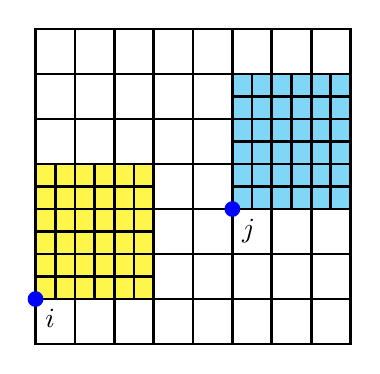
\begin{tikzpicture}[scale=4.0]
    % Define layers
    \pgfdeclarelayer{background}
    \pgfsetlayers{background,main}

    \coordinate (v1_1) at (0.0, 0.0);
    \coordinate (v1_2) at (0.125, 0.0);
    \coordinate (v1_3) at (0.125, 0.14285714285714285);
    \coordinate (v1_4) at (0.0, 0.14285714285714285);
    \draw[black, line width=1.0pt] (v1_1) -- (v1_2) -- (v1_3) -- (v1_4) -- cycle;
    \coordinate (v2_1) at (0.125, 0.0);
    \coordinate (v2_2) at (0.25, 0.0);
    \coordinate (v2_3) at (0.25, 0.14285714285714285);
    \coordinate (v2_4) at (0.125, 0.14285714285714285);
    \draw[black, line width=1.0pt] (v2_1) -- (v2_2) -- (v2_3) -- (v2_4) -- cycle;
    \coordinate (v3_1) at (0.25, 0.0);
    \coordinate (v3_2) at (0.375, 0.0);
    \coordinate (v3_3) at (0.375, 0.14285714285714285);
    \coordinate (v3_4) at (0.25, 0.14285714285714285);
    \draw[black, line width=1.0pt] (v3_1) -- (v3_2) -- (v3_3) -- (v3_4) -- cycle;
    \coordinate (v4_1) at (0.375, 0.0);
    \coordinate (v4_2) at (0.5, 0.0);
    \coordinate (v4_3) at (0.5, 0.14285714285714285);
    \coordinate (v4_4) at (0.375, 0.14285714285714285);
    \draw[black, line width=1.0pt] (v4_1) -- (v4_2) -- (v4_3) -- (v4_4) -- cycle;
    \coordinate (v5_1) at (0.5, 0.0);
    \coordinate (v5_2) at (0.625, 0.0);
    \coordinate (v5_3) at (0.625, 0.14285714285714285);
    \coordinate (v5_4) at (0.5, 0.14285714285714285);
    \draw[black, line width=1.0pt] (v5_1) -- (v5_2) -- (v5_3) -- (v5_4) -- cycle;
    \coordinate (v6_1) at (0.625, 0.0);
    \coordinate (v6_2) at (0.75, 0.0);
    \coordinate (v6_3) at (0.75, 0.14285714285714285);
    \coordinate (v6_4) at (0.625, 0.14285714285714285);
    \draw[black, line width=1.0pt] (v6_1) -- (v6_2) -- (v6_3) -- (v6_4) -- cycle;
    \coordinate (v7_1) at (0.75, 0.0);
    \coordinate (v7_2) at (0.875, 0.0);
    \coordinate (v7_3) at (0.875, 0.14285714285714285);
    \coordinate (v7_4) at (0.75, 0.14285714285714285);
    \draw[black, line width=1.0pt] (v7_1) -- (v7_2) -- (v7_3) -- (v7_4) -- cycle;
    \coordinate (v8_1) at (0.875, 0.0);
    \coordinate (v8_2) at (1.0, 0.0);
    \coordinate (v8_3) at (1.0, 0.14285714285714285);
    \coordinate (v8_4) at (0.875, 0.14285714285714285);
    \draw[black, line width=1.0pt] (v8_1) -- (v8_2) -- (v8_3) -- (v8_4) -- cycle;
    \coordinate (v9_1) at (0.375, 0.14285714285714285);
    \coordinate (v9_2) at (0.5, 0.14285714285714285);
    \coordinate (v9_3) at (0.5, 0.2857142857142857);
    \coordinate (v9_4) at (0.375, 0.2857142857142857);
    \draw[black, line width=1.0pt] (v9_1) -- (v9_2) -- (v9_3) -- (v9_4) -- cycle;
    \coordinate (v10_1) at (0.5, 0.14285714285714285);
    \coordinate (v10_2) at (0.625, 0.14285714285714285);
    \coordinate (v10_3) at (0.625, 0.2857142857142857);
    \coordinate (v10_4) at (0.5, 0.2857142857142857);
    \draw[black, line width=1.0pt] (v10_1) -- (v10_2) -- (v10_3) -- (v10_4) -- cycle;
    \coordinate (v11_1) at (0.625, 0.14285714285714285);
    \coordinate (v11_2) at (0.75, 0.14285714285714285);
    \coordinate (v11_3) at (0.75, 0.2857142857142857);
    \coordinate (v11_4) at (0.625, 0.2857142857142857);
    \draw[black, line width=1.0pt] (v11_1) -- (v11_2) -- (v11_3) -- (v11_4) -- cycle;
    \coordinate (v12_1) at (0.75, 0.14285714285714285);
    \coordinate (v12_2) at (0.875, 0.14285714285714285);
    \coordinate (v12_3) at (0.875, 0.2857142857142857);
    \coordinate (v12_4) at (0.75, 0.2857142857142857);
    \draw[black, line width=1.0pt] (v12_1) -- (v12_2) -- (v12_3) -- (v12_4) -- cycle;
    \coordinate (v13_1) at (0.875, 0.14285714285714285);
    \coordinate (v13_2) at (1.0, 0.14285714285714285);
    \coordinate (v13_3) at (1.0, 0.2857142857142857);
    \coordinate (v13_4) at (0.875, 0.2857142857142857);
    \draw[black, line width=1.0pt] (v13_1) -- (v13_2) -- (v13_3) -- (v13_4) -- cycle;
    \coordinate (v14_1) at (0.375, 0.2857142857142857);
    \coordinate (v14_2) at (0.5, 0.2857142857142857);
    \coordinate (v14_3) at (0.5, 0.42857142857142855);
    \coordinate (v14_4) at (0.375, 0.42857142857142855);
    \draw[black, line width=1.0pt] (v14_1) -- (v14_2) -- (v14_3) -- (v14_4) -- cycle;
    \coordinate (v15_1) at (0.5, 0.2857142857142857);
    \coordinate (v15_2) at (0.625, 0.2857142857142857);
    \coordinate (v15_3) at (0.625, 0.42857142857142855);
    \coordinate (v15_4) at (0.5, 0.42857142857142855);
    \draw[black, line width=1.0pt] (v15_1) -- (v15_2) -- (v15_3) -- (v15_4) -- cycle;
    \coordinate (v16_1) at (0.625, 0.2857142857142857);
    \coordinate (v16_2) at (0.75, 0.2857142857142857);
    \coordinate (v16_3) at (0.75, 0.42857142857142855);
    \coordinate (v16_4) at (0.625, 0.42857142857142855);
    \draw[black, line width=1.0pt] (v16_1) -- (v16_2) -- (v16_3) -- (v16_4) -- cycle;
    \coordinate (v17_1) at (0.75, 0.2857142857142857);
    \coordinate (v17_2) at (0.875, 0.2857142857142857);
    \coordinate (v17_3) at (0.875, 0.42857142857142855);
    \coordinate (v17_4) at (0.75, 0.42857142857142855);
    \draw[black, line width=1.0pt] (v17_1) -- (v17_2) -- (v17_3) -- (v17_4) -- cycle;
    \coordinate (v18_1) at (0.875, 0.2857142857142857);
    \coordinate (v18_2) at (1.0, 0.2857142857142857);
    \coordinate (v18_3) at (1.0, 0.42857142857142855);
    \coordinate (v18_4) at (0.875, 0.42857142857142855);
    \draw[black, line width=1.0pt] (v18_1) -- (v18_2) -- (v18_3) -- (v18_4) -- cycle;
    \coordinate (v19_1) at (0.375, 0.42857142857142855);
    \coordinate (v19_2) at (0.5, 0.42857142857142855);
    \coordinate (v19_3) at (0.5, 0.5714285714285714);
    \coordinate (v19_4) at (0.375, 0.5714285714285714);
    \draw[black, line width=1.0pt] (v19_1) -- (v19_2) -- (v19_3) -- (v19_4) -- cycle;
    \coordinate (v20_1) at (0.5, 0.42857142857142855);
    \coordinate (v20_2) at (0.625, 0.42857142857142855);
    \coordinate (v20_3) at (0.625, 0.5714285714285714);
    \coordinate (v20_4) at (0.5, 0.5714285714285714);
    \draw[black, line width=1.0pt] (v20_1) -- (v20_2) -- (v20_3) -- (v20_4) -- cycle;
    \coordinate (v21_1) at (0.0, 0.5714285714285714);
    \coordinate (v21_2) at (0.125, 0.5714285714285714);
    \coordinate (v21_3) at (0.125, 0.7142857142857143);
    \coordinate (v21_4) at (0.0, 0.7142857142857143);
    \draw[black, line width=1.0pt] (v21_1) -- (v21_2) -- (v21_3) -- (v21_4) -- cycle;
    \coordinate (v22_1) at (0.125, 0.5714285714285714);
    \coordinate (v22_2) at (0.25, 0.5714285714285714);
    \coordinate (v22_3) at (0.25, 0.7142857142857143);
    \coordinate (v22_4) at (0.125, 0.7142857142857143);
    \draw[black, line width=1.0pt] (v22_1) -- (v22_2) -- (v22_3) -- (v22_4) -- cycle;
    \coordinate (v23_1) at (0.25, 0.5714285714285714);
    \coordinate (v23_2) at (0.375, 0.5714285714285714);
    \coordinate (v23_3) at (0.375, 0.7142857142857143);
    \coordinate (v23_4) at (0.25, 0.7142857142857143);
    \draw[black, line width=1.0pt] (v23_1) -- (v23_2) -- (v23_3) -- (v23_4) -- cycle;
    \coordinate (v24_1) at (0.375, 0.5714285714285714);
    \coordinate (v24_2) at (0.5, 0.5714285714285714);
    \coordinate (v24_3) at (0.5, 0.7142857142857143);
    \coordinate (v24_4) at (0.375, 0.7142857142857143);
    \draw[black, line width=1.0pt] (v24_1) -- (v24_2) -- (v24_3) -- (v24_4) -- cycle;
    \coordinate (v25_1) at (0.5, 0.5714285714285714);
    \coordinate (v25_2) at (0.625, 0.5714285714285714);
    \coordinate (v25_3) at (0.625, 0.7142857142857143);
    \coordinate (v25_4) at (0.5, 0.7142857142857143);
    \draw[black, line width=1.0pt] (v25_1) -- (v25_2) -- (v25_3) -- (v25_4) -- cycle;
    \coordinate (v26_1) at (0.0, 0.7142857142857143);
    \coordinate (v26_2) at (0.125, 0.7142857142857143);
    \coordinate (v26_3) at (0.125, 0.8571428571428571);
    \coordinate (v26_4) at (0.0, 0.8571428571428571);
    \draw[black, line width=1.0pt] (v26_1) -- (v26_2) -- (v26_3) -- (v26_4) -- cycle;
    \coordinate (v27_1) at (0.125, 0.7142857142857143);
    \coordinate (v27_2) at (0.25, 0.7142857142857143);
    \coordinate (v27_3) at (0.25, 0.8571428571428571);
    \coordinate (v27_4) at (0.125, 0.8571428571428571);
    \draw[black, line width=1.0pt] (v27_1) -- (v27_2) -- (v27_3) -- (v27_4) -- cycle;
    \coordinate (v28_1) at (0.25, 0.7142857142857143);
    \coordinate (v28_2) at (0.375, 0.7142857142857143);
    \coordinate (v28_3) at (0.375, 0.8571428571428571);
    \coordinate (v28_4) at (0.25, 0.8571428571428571);
    \draw[black, line width=1.0pt] (v28_1) -- (v28_2) -- (v28_3) -- (v28_4) -- cycle;
    \coordinate (v29_1) at (0.375, 0.7142857142857143);
    \coordinate (v29_2) at (0.5, 0.7142857142857143);
    \coordinate (v29_3) at (0.5, 0.8571428571428571);
    \coordinate (v29_4) at (0.375, 0.8571428571428571);
    \draw[black, line width=1.0pt] (v29_1) -- (v29_2) -- (v29_3) -- (v29_4) -- cycle;
    \coordinate (v30_1) at (0.5, 0.7142857142857143);
    \coordinate (v30_2) at (0.625, 0.7142857142857143);
    \coordinate (v30_3) at (0.625, 0.8571428571428571);
    \coordinate (v30_4) at (0.5, 0.8571428571428571);
    \draw[black, line width=1.0pt] (v30_1) -- (v30_2) -- (v30_3) -- (v30_4) -- cycle;
    \coordinate (v31_1) at (0.0, 0.8571428571428571);
    \coordinate (v31_2) at (0.125, 0.8571428571428571);
    \coordinate (v31_3) at (0.125, 1.0);
    \coordinate (v31_4) at (0.0, 1.0);
    \draw[black, line width=1.0pt] (v31_1) -- (v31_2) -- (v31_3) -- (v31_4) -- cycle;
    \coordinate (v32_1) at (0.125, 0.8571428571428571);
    \coordinate (v32_2) at (0.25, 0.8571428571428571);
    \coordinate (v32_3) at (0.25, 1.0);
    \coordinate (v32_4) at (0.125, 1.0);
    \draw[black, line width=1.0pt] (v32_1) -- (v32_2) -- (v32_3) -- (v32_4) -- cycle;
    \coordinate (v33_1) at (0.25, 0.8571428571428571);
    \coordinate (v33_2) at (0.375, 0.8571428571428571);
    \coordinate (v33_3) at (0.375, 1.0);
    \coordinate (v33_4) at (0.25, 1.0);
    \draw[black, line width=1.0pt] (v33_1) -- (v33_2) -- (v33_3) -- (v33_4) -- cycle;
    \coordinate (v34_1) at (0.375, 0.8571428571428571);
    \coordinate (v34_2) at (0.5, 0.8571428571428571);
    \coordinate (v34_3) at (0.5, 1.0);
    \coordinate (v34_4) at (0.375, 1.0);
    \draw[black, line width=1.0pt] (v34_1) -- (v34_2) -- (v34_3) -- (v34_4) -- cycle;
    \coordinate (v35_1) at (0.5, 0.8571428571428571);
    \coordinate (v35_2) at (0.625, 0.8571428571428571);
    \coordinate (v35_3) at (0.625, 1.0);
    \coordinate (v35_4) at (0.5, 1.0);
    \draw[black, line width=1.0pt] (v35_1) -- (v35_2) -- (v35_3) -- (v35_4) -- cycle;
    \coordinate (v36_1) at (0.625, 0.8571428571428571);
    \coordinate (v36_2) at (0.75, 0.8571428571428571);
    \coordinate (v36_3) at (0.75, 1.0);
    \coordinate (v36_4) at (0.625, 1.0);
    \draw[black, line width=1.0pt] (v36_1) -- (v36_2) -- (v36_3) -- (v36_4) -- cycle;
    \coordinate (v37_1) at (0.75, 0.8571428571428571);
    \coordinate (v37_2) at (0.875, 0.8571428571428571);
    \coordinate (v37_3) at (0.875, 1.0);
    \coordinate (v37_4) at (0.75, 1.0);
    \draw[black, line width=1.0pt] (v37_1) -- (v37_2) -- (v37_3) -- (v37_4) -- cycle;
    \coordinate (v38_1) at (0.875, 0.8571428571428571);
    \coordinate (v38_2) at (1.0, 0.8571428571428571);
    \coordinate (v38_3) at (1.0, 1.0);
    \coordinate (v38_4) at (0.875, 1.0);
    \draw[black, line width=1.0pt] (v38_1) -- (v38_2) -- (v38_3) -- (v38_4) -- cycle;
    \coordinate (v39_1) at (0.0, 0.14285714285714285);
    \coordinate (v39_2) at (0.0625, 0.14285714285714285);
    \coordinate (v39_3) at (0.0625, 0.21428571428571427);
    \coordinate (v39_4) at (0.0, 0.21428571428571427);
    \draw[black, line width=1.0pt] (v39_1) -- (v39_2) -- (v39_3) -- (v39_4) -- cycle;
    \coordinate (v40_1) at (0.0625, 0.14285714285714285);
    \coordinate (v40_2) at (0.125, 0.14285714285714285);
    \coordinate (v40_3) at (0.125, 0.21428571428571427);
    \coordinate (v40_4) at (0.0625, 0.21428571428571427);
    \draw[black, line width=1.0pt] (v40_1) -- (v40_2) -- (v40_3) -- (v40_4) -- cycle;
    \coordinate (v41_1) at (0.125, 0.14285714285714285);
    \coordinate (v41_2) at (0.1875, 0.14285714285714285);
    \coordinate (v41_3) at (0.1875, 0.21428571428571427);
    \coordinate (v41_4) at (0.125, 0.21428571428571427);
    \draw[black, line width=1.0pt] (v41_1) -- (v41_2) -- (v41_3) -- (v41_4) -- cycle;
    \coordinate (v42_1) at (0.1875, 0.14285714285714285);
    \coordinate (v42_2) at (0.25, 0.14285714285714285);
    \coordinate (v42_3) at (0.25, 0.21428571428571427);
    \coordinate (v42_4) at (0.1875, 0.21428571428571427);
    \draw[black, line width=1.0pt] (v42_1) -- (v42_2) -- (v42_3) -- (v42_4) -- cycle;
    \coordinate (v43_1) at (0.25, 0.14285714285714285);
    \coordinate (v43_2) at (0.3125, 0.14285714285714285);
    \coordinate (v43_3) at (0.3125, 0.21428571428571427);
    \coordinate (v43_4) at (0.25, 0.21428571428571427);
    \draw[black, line width=1.0pt] (v43_1) -- (v43_2) -- (v43_3) -- (v43_4) -- cycle;
    \coordinate (v44_1) at (0.3125, 0.14285714285714285);
    \coordinate (v44_2) at (0.375, 0.14285714285714285);
    \coordinate (v44_3) at (0.375, 0.21428571428571427);
    \coordinate (v44_4) at (0.3125, 0.21428571428571427);
    \draw[black, line width=1.0pt] (v44_1) -- (v44_2) -- (v44_3) -- (v44_4) -- cycle;
    \coordinate (v45_1) at (0.0, 0.21428571428571427);
    \coordinate (v45_2) at (0.0625, 0.21428571428571427);
    \coordinate (v45_3) at (0.0625, 0.2857142857142857);
    \coordinate (v45_4) at (0.0, 0.2857142857142857);
    \draw[black, line width=1.0pt] (v45_1) -- (v45_2) -- (v45_3) -- (v45_4) -- cycle;
    \coordinate (v46_1) at (0.0625, 0.21428571428571427);
    \coordinate (v46_2) at (0.125, 0.21428571428571427);
    \coordinate (v46_3) at (0.125, 0.2857142857142857);
    \coordinate (v46_4) at (0.0625, 0.2857142857142857);
    \draw[black, line width=1.0pt] (v46_1) -- (v46_2) -- (v46_3) -- (v46_4) -- cycle;
    \coordinate (v47_1) at (0.125, 0.21428571428571427);
    \coordinate (v47_2) at (0.1875, 0.21428571428571427);
    \coordinate (v47_3) at (0.1875, 0.2857142857142857);
    \coordinate (v47_4) at (0.125, 0.2857142857142857);
    \draw[black, line width=1.0pt] (v47_1) -- (v47_2) -- (v47_3) -- (v47_4) -- cycle;
    \coordinate (v48_1) at (0.1875, 0.21428571428571427);
    \coordinate (v48_2) at (0.25, 0.21428571428571427);
    \coordinate (v48_3) at (0.25, 0.2857142857142857);
    \coordinate (v48_4) at (0.1875, 0.2857142857142857);
    \draw[black, line width=1.0pt] (v48_1) -- (v48_2) -- (v48_3) -- (v48_4) -- cycle;
    \coordinate (v49_1) at (0.25, 0.21428571428571427);
    \coordinate (v49_2) at (0.3125, 0.21428571428571427);
    \coordinate (v49_3) at (0.3125, 0.2857142857142857);
    \coordinate (v49_4) at (0.25, 0.2857142857142857);
    \draw[black, line width=1.0pt] (v49_1) -- (v49_2) -- (v49_3) -- (v49_4) -- cycle;
    \coordinate (v50_1) at (0.3125, 0.21428571428571427);
    \coordinate (v50_2) at (0.375, 0.21428571428571427);
    \coordinate (v50_3) at (0.375, 0.2857142857142857);
    \coordinate (v50_4) at (0.3125, 0.2857142857142857);
    \draw[black, line width=1.0pt] (v50_1) -- (v50_2) -- (v50_3) -- (v50_4) -- cycle;
    \coordinate (v51_1) at (0.0, 0.2857142857142857);
    \coordinate (v51_2) at (0.0625, 0.2857142857142857);
    \coordinate (v51_3) at (0.0625, 0.3571428571428571);
    \coordinate (v51_4) at (0.0, 0.3571428571428571);
    \draw[black, line width=1.0pt] (v51_1) -- (v51_2) -- (v51_3) -- (v51_4) -- cycle;
    \coordinate (v52_1) at (0.0625, 0.2857142857142857);
    \coordinate (v52_2) at (0.125, 0.2857142857142857);
    \coordinate (v52_3) at (0.125, 0.3571428571428571);
    \coordinate (v52_4) at (0.0625, 0.3571428571428571);
    \draw[black, line width=1.0pt] (v52_1) -- (v52_2) -- (v52_3) -- (v52_4) -- cycle;
    \coordinate (v53_1) at (0.125, 0.2857142857142857);
    \coordinate (v53_2) at (0.1875, 0.2857142857142857);
    \coordinate (v53_3) at (0.1875, 0.3571428571428571);
    \coordinate (v53_4) at (0.125, 0.3571428571428571);
    \draw[black, line width=1.0pt] (v53_1) -- (v53_2) -- (v53_3) -- (v53_4) -- cycle;
    \coordinate (v54_1) at (0.1875, 0.2857142857142857);
    \coordinate (v54_2) at (0.25, 0.2857142857142857);
    \coordinate (v54_3) at (0.25, 0.3571428571428571);
    \coordinate (v54_4) at (0.1875, 0.3571428571428571);
    \draw[black, line width=1.0pt] (v54_1) -- (v54_2) -- (v54_3) -- (v54_4) -- cycle;
    \coordinate (v55_1) at (0.25, 0.2857142857142857);
    \coordinate (v55_2) at (0.3125, 0.2857142857142857);
    \coordinate (v55_3) at (0.3125, 0.3571428571428571);
    \coordinate (v55_4) at (0.25, 0.3571428571428571);
    \draw[black, line width=1.0pt] (v55_1) -- (v55_2) -- (v55_3) -- (v55_4) -- cycle;
    \coordinate (v56_1) at (0.3125, 0.2857142857142857);
    \coordinate (v56_2) at (0.375, 0.2857142857142857);
    \coordinate (v56_3) at (0.375, 0.3571428571428571);
    \coordinate (v56_4) at (0.3125, 0.3571428571428571);
    \draw[black, line width=1.0pt] (v56_1) -- (v56_2) -- (v56_3) -- (v56_4) -- cycle;
    \coordinate (v57_1) at (0.0, 0.3571428571428571);
    \coordinate (v57_2) at (0.0625, 0.3571428571428571);
    \coordinate (v57_3) at (0.0625, 0.42857142857142855);
    \coordinate (v57_4) at (0.0, 0.42857142857142855);
    \draw[black, line width=1.0pt] (v57_1) -- (v57_2) -- (v57_3) -- (v57_4) -- cycle;
    \coordinate (v58_1) at (0.0625, 0.3571428571428571);
    \coordinate (v58_2) at (0.125, 0.3571428571428571);
    \coordinate (v58_3) at (0.125, 0.42857142857142855);
    \coordinate (v58_4) at (0.0625, 0.42857142857142855);
    \draw[black, line width=1.0pt] (v58_1) -- (v58_2) -- (v58_3) -- (v58_4) -- cycle;
    \coordinate (v59_1) at (0.125, 0.3571428571428571);
    \coordinate (v59_2) at (0.1875, 0.3571428571428571);
    \coordinate (v59_3) at (0.1875, 0.42857142857142855);
    \coordinate (v59_4) at (0.125, 0.42857142857142855);
    \draw[black, line width=1.0pt] (v59_1) -- (v59_2) -- (v59_3) -- (v59_4) -- cycle;
    \coordinate (v60_1) at (0.1875, 0.3571428571428571);
    \coordinate (v60_2) at (0.25, 0.3571428571428571);
    \coordinate (v60_3) at (0.25, 0.42857142857142855);
    \coordinate (v60_4) at (0.1875, 0.42857142857142855);
    \draw[black, line width=1.0pt] (v60_1) -- (v60_2) -- (v60_3) -- (v60_4) -- cycle;
    \coordinate (v61_1) at (0.25, 0.3571428571428571);
    \coordinate (v61_2) at (0.3125, 0.3571428571428571);
    \coordinate (v61_3) at (0.3125, 0.42857142857142855);
    \coordinate (v61_4) at (0.25, 0.42857142857142855);
    \draw[black, line width=1.0pt] (v61_1) -- (v61_2) -- (v61_3) -- (v61_4) -- cycle;
    \coordinate (v62_1) at (0.3125, 0.3571428571428571);
    \coordinate (v62_2) at (0.375, 0.3571428571428571);
    \coordinate (v62_3) at (0.375, 0.42857142857142855);
    \coordinate (v62_4) at (0.3125, 0.42857142857142855);
    \draw[black, line width=1.0pt] (v62_1) -- (v62_2) -- (v62_3) -- (v62_4) -- cycle;
    \coordinate (v63_1) at (0.0, 0.42857142857142855);
    \coordinate (v63_2) at (0.0625, 0.42857142857142855);
    \coordinate (v63_3) at (0.0625, 0.5);
    \coordinate (v63_4) at (0.0, 0.5);
    \draw[black, line width=1.0pt] (v63_1) -- (v63_2) -- (v63_3) -- (v63_4) -- cycle;
    \coordinate (v64_1) at (0.0625, 0.42857142857142855);
    \coordinate (v64_2) at (0.125, 0.42857142857142855);
    \coordinate (v64_3) at (0.125, 0.5);
    \coordinate (v64_4) at (0.0625, 0.5);
    \draw[black, line width=1.0pt] (v64_1) -- (v64_2) -- (v64_3) -- (v64_4) -- cycle;
    \coordinate (v65_1) at (0.125, 0.42857142857142855);
    \coordinate (v65_2) at (0.1875, 0.42857142857142855);
    \coordinate (v65_3) at (0.1875, 0.5);
    \coordinate (v65_4) at (0.125, 0.5);
    \draw[black, line width=1.0pt] (v65_1) -- (v65_2) -- (v65_3) -- (v65_4) -- cycle;
    \coordinate (v66_1) at (0.1875, 0.42857142857142855);
    \coordinate (v66_2) at (0.25, 0.42857142857142855);
    \coordinate (v66_3) at (0.25, 0.5);
    \coordinate (v66_4) at (0.1875, 0.5);
    \draw[black, line width=1.0pt] (v66_1) -- (v66_2) -- (v66_3) -- (v66_4) -- cycle;
    \coordinate (v67_1) at (0.25, 0.42857142857142855);
    \coordinate (v67_2) at (0.3125, 0.42857142857142855);
    \coordinate (v67_3) at (0.3125, 0.5);
    \coordinate (v67_4) at (0.25, 0.5);
    \draw[black, line width=1.0pt] (v67_1) -- (v67_2) -- (v67_3) -- (v67_4) -- cycle;
    \coordinate (v68_1) at (0.3125, 0.42857142857142855);
    \coordinate (v68_2) at (0.375, 0.42857142857142855);
    \coordinate (v68_3) at (0.375, 0.5);
    \coordinate (v68_4) at (0.3125, 0.5);
    \draw[black, line width=1.0pt] (v68_1) -- (v68_2) -- (v68_3) -- (v68_4) -- cycle;
    \coordinate (v69_1) at (0.625, 0.42857142857142855);
    \coordinate (v69_2) at (0.6875, 0.42857142857142855);
    \coordinate (v69_3) at (0.6875, 0.5);
    \coordinate (v69_4) at (0.625, 0.5);
    \draw[black, line width=1.0pt] (v69_1) -- (v69_2) -- (v69_3) -- (v69_4) -- cycle;
    \coordinate (v70_1) at (0.6875, 0.42857142857142855);
    \coordinate (v70_2) at (0.75, 0.42857142857142855);
    \coordinate (v70_3) at (0.75, 0.5);
    \coordinate (v70_4) at (0.6875, 0.5);
    \draw[black, line width=1.0pt] (v70_1) -- (v70_2) -- (v70_3) -- (v70_4) -- cycle;
    \coordinate (v71_1) at (0.75, 0.42857142857142855);
    \coordinate (v71_2) at (0.8125, 0.42857142857142855);
    \coordinate (v71_3) at (0.8125, 0.5);
    \coordinate (v71_4) at (0.75, 0.5);
    \draw[black, line width=1.0pt] (v71_1) -- (v71_2) -- (v71_3) -- (v71_4) -- cycle;
    \coordinate (v72_1) at (0.8125, 0.42857142857142855);
    \coordinate (v72_2) at (0.875, 0.42857142857142855);
    \coordinate (v72_3) at (0.875, 0.5);
    \coordinate (v72_4) at (0.8125, 0.5);
    \draw[black, line width=1.0pt] (v72_1) -- (v72_2) -- (v72_3) -- (v72_4) -- cycle;
    \coordinate (v73_1) at (0.875, 0.42857142857142855);
    \coordinate (v73_2) at (0.9375, 0.42857142857142855);
    \coordinate (v73_3) at (0.9375, 0.5);
    \coordinate (v73_4) at (0.875, 0.5);
    \draw[black, line width=1.0pt] (v73_1) -- (v73_2) -- (v73_3) -- (v73_4) -- cycle;
    \coordinate (v74_1) at (0.9375, 0.42857142857142855);
    \coordinate (v74_2) at (1.0, 0.42857142857142855);
    \coordinate (v74_3) at (1.0, 0.5);
    \coordinate (v74_4) at (0.9375, 0.5);
    \draw[black, line width=1.0pt] (v74_1) -- (v74_2) -- (v74_3) -- (v74_4) -- cycle;
    \coordinate (v75_1) at (0.0, 0.5);
    \coordinate (v75_2) at (0.0625, 0.5);
    \coordinate (v75_3) at (0.0625, 0.5714285714285714);
    \coordinate (v75_4) at (0.0, 0.5714285714285714);
    \draw[black, line width=1.0pt] (v75_1) -- (v75_2) -- (v75_3) -- (v75_4) -- cycle;
    \coordinate (v76_1) at (0.0625, 0.5);
    \coordinate (v76_2) at (0.125, 0.5);
    \coordinate (v76_3) at (0.125, 0.5714285714285714);
    \coordinate (v76_4) at (0.0625, 0.5714285714285714);
    \draw[black, line width=1.0pt] (v76_1) -- (v76_2) -- (v76_3) -- (v76_4) -- cycle;
    \coordinate (v77_1) at (0.125, 0.5);
    \coordinate (v77_2) at (0.1875, 0.5);
    \coordinate (v77_3) at (0.1875, 0.5714285714285714);
    \coordinate (v77_4) at (0.125, 0.5714285714285714);
    \draw[black, line width=1.0pt] (v77_1) -- (v77_2) -- (v77_3) -- (v77_4) -- cycle;
    \coordinate (v78_1) at (0.1875, 0.5);
    \coordinate (v78_2) at (0.25, 0.5);
    \coordinate (v78_3) at (0.25, 0.5714285714285714);
    \coordinate (v78_4) at (0.1875, 0.5714285714285714);
    \draw[black, line width=1.0pt] (v78_1) -- (v78_2) -- (v78_3) -- (v78_4) -- cycle;
    \coordinate (v79_1) at (0.25, 0.5);
    \coordinate (v79_2) at (0.3125, 0.5);
    \coordinate (v79_3) at (0.3125, 0.5714285714285714);
    \coordinate (v79_4) at (0.25, 0.5714285714285714);
    \draw[black, line width=1.0pt] (v79_1) -- (v79_2) -- (v79_3) -- (v79_4) -- cycle;
    \coordinate (v80_1) at (0.3125, 0.5);
    \coordinate (v80_2) at (0.375, 0.5);
    \coordinate (v80_3) at (0.375, 0.5714285714285714);
    \coordinate (v80_4) at (0.3125, 0.5714285714285714);
    \draw[black, line width=1.0pt] (v80_1) -- (v80_2) -- (v80_3) -- (v80_4) -- cycle;
    \coordinate (v81_1) at (0.625, 0.5);
    \coordinate (v81_2) at (0.6875, 0.5);
    \coordinate (v81_3) at (0.6875, 0.5714285714285714);
    \coordinate (v81_4) at (0.625, 0.5714285714285714);
    \draw[black, line width=1.0pt] (v81_1) -- (v81_2) -- (v81_3) -- (v81_4) -- cycle;
    \coordinate (v82_1) at (0.6875, 0.5);
    \coordinate (v82_2) at (0.75, 0.5);
    \coordinate (v82_3) at (0.75, 0.5714285714285714);
    \coordinate (v82_4) at (0.6875, 0.5714285714285714);
    \draw[black, line width=1.0pt] (v82_1) -- (v82_2) -- (v82_3) -- (v82_4) -- cycle;
    \coordinate (v83_1) at (0.75, 0.5);
    \coordinate (v83_2) at (0.8125, 0.5);
    \coordinate (v83_3) at (0.8125, 0.5714285714285714);
    \coordinate (v83_4) at (0.75, 0.5714285714285714);
    \draw[black, line width=1.0pt] (v83_1) -- (v83_2) -- (v83_3) -- (v83_4) -- cycle;
    \coordinate (v84_1) at (0.8125, 0.5);
    \coordinate (v84_2) at (0.875, 0.5);
    \coordinate (v84_3) at (0.875, 0.5714285714285714);
    \coordinate (v84_4) at (0.8125, 0.5714285714285714);
    \draw[black, line width=1.0pt] (v84_1) -- (v84_2) -- (v84_3) -- (v84_4) -- cycle;
    \coordinate (v85_1) at (0.875, 0.5);
    \coordinate (v85_2) at (0.9375, 0.5);
    \coordinate (v85_3) at (0.9375, 0.5714285714285714);
    \coordinate (v85_4) at (0.875, 0.5714285714285714);
    \draw[black, line width=1.0pt] (v85_1) -- (v85_2) -- (v85_3) -- (v85_4) -- cycle;
    \coordinate (v86_1) at (0.9375, 0.5);
    \coordinate (v86_2) at (1.0, 0.5);
    \coordinate (v86_3) at (1.0, 0.5714285714285714);
    \coordinate (v86_4) at (0.9375, 0.5714285714285714);
    \draw[black, line width=1.0pt] (v86_1) -- (v86_2) -- (v86_3) -- (v86_4) -- cycle;
    \coordinate (v87_1) at (0.625, 0.5714285714285714);
    \coordinate (v87_2) at (0.6875, 0.5714285714285714);
    \coordinate (v87_3) at (0.6875, 0.6428571428571428);
    \coordinate (v87_4) at (0.625, 0.6428571428571428);
    \draw[black, line width=1.0pt] (v87_1) -- (v87_2) -- (v87_3) -- (v87_4) -- cycle;
    \coordinate (v88_1) at (0.6875, 0.5714285714285714);
    \coordinate (v88_2) at (0.75, 0.5714285714285714);
    \coordinate (v88_3) at (0.75, 0.6428571428571428);
    \coordinate (v88_4) at (0.6875, 0.6428571428571428);
    \draw[black, line width=1.0pt] (v88_1) -- (v88_2) -- (v88_3) -- (v88_4) -- cycle;
    \coordinate (v89_1) at (0.75, 0.5714285714285714);
    \coordinate (v89_2) at (0.8125, 0.5714285714285714);
    \coordinate (v89_3) at (0.8125, 0.6428571428571428);
    \coordinate (v89_4) at (0.75, 0.6428571428571428);
    \draw[black, line width=1.0pt] (v89_1) -- (v89_2) -- (v89_3) -- (v89_4) -- cycle;
    \coordinate (v90_1) at (0.8125, 0.5714285714285714);
    \coordinate (v90_2) at (0.875, 0.5714285714285714);
    \coordinate (v90_3) at (0.875, 0.6428571428571428);
    \coordinate (v90_4) at (0.8125, 0.6428571428571428);
    \draw[black, line width=1.0pt] (v90_1) -- (v90_2) -- (v90_3) -- (v90_4) -- cycle;
    \coordinate (v91_1) at (0.875, 0.5714285714285714);
    \coordinate (v91_2) at (0.9375, 0.5714285714285714);
    \coordinate (v91_3) at (0.9375, 0.6428571428571428);
    \coordinate (v91_4) at (0.875, 0.6428571428571428);
    \draw[black, line width=1.0pt] (v91_1) -- (v91_2) -- (v91_3) -- (v91_4) -- cycle;
    \coordinate (v92_1) at (0.9375, 0.5714285714285714);
    \coordinate (v92_2) at (1.0, 0.5714285714285714);
    \coordinate (v92_3) at (1.0, 0.6428571428571428);
    \coordinate (v92_4) at (0.9375, 0.6428571428571428);
    \draw[black, line width=1.0pt] (v92_1) -- (v92_2) -- (v92_3) -- (v92_4) -- cycle;
    \coordinate (v93_1) at (0.625, 0.6428571428571428);
    \coordinate (v93_2) at (0.6875, 0.6428571428571428);
    \coordinate (v93_3) at (0.6875, 0.7142857142857143);
    \coordinate (v93_4) at (0.625, 0.7142857142857143);
    \draw[black, line width=1.0pt] (v93_1) -- (v93_2) -- (v93_3) -- (v93_4) -- cycle;
    \coordinate (v94_1) at (0.6875, 0.6428571428571428);
    \coordinate (v94_2) at (0.75, 0.6428571428571428);
    \coordinate (v94_3) at (0.75, 0.7142857142857143);
    \coordinate (v94_4) at (0.6875, 0.7142857142857143);
    \draw[black, line width=1.0pt] (v94_1) -- (v94_2) -- (v94_3) -- (v94_4) -- cycle;
    \coordinate (v95_1) at (0.75, 0.6428571428571428);
    \coordinate (v95_2) at (0.8125, 0.6428571428571428);
    \coordinate (v95_3) at (0.8125, 0.7142857142857143);
    \coordinate (v95_4) at (0.75, 0.7142857142857143);
    \draw[black, line width=1.0pt] (v95_1) -- (v95_2) -- (v95_3) -- (v95_4) -- cycle;
    \coordinate (v96_1) at (0.8125, 0.6428571428571428);
    \coordinate (v96_2) at (0.875, 0.6428571428571428);
    \coordinate (v96_3) at (0.875, 0.7142857142857143);
    \coordinate (v96_4) at (0.8125, 0.7142857142857143);
    \draw[black, line width=1.0pt] (v96_1) -- (v96_2) -- (v96_3) -- (v96_4) -- cycle;
    \coordinate (v97_1) at (0.875, 0.6428571428571428);
    \coordinate (v97_2) at (0.9375, 0.6428571428571428);
    \coordinate (v97_3) at (0.9375, 0.7142857142857143);
    \coordinate (v97_4) at (0.875, 0.7142857142857143);
    \draw[black, line width=1.0pt] (v97_1) -- (v97_2) -- (v97_3) -- (v97_4) -- cycle;
    \coordinate (v98_1) at (0.9375, 0.6428571428571428);
    \coordinate (v98_2) at (1.0, 0.6428571428571428);
    \coordinate (v98_3) at (1.0, 0.7142857142857143);
    \coordinate (v98_4) at (0.9375, 0.7142857142857143);
    \draw[black, line width=1.0pt] (v98_1) -- (v98_2) -- (v98_3) -- (v98_4) -- cycle;
    \coordinate (v99_1) at (0.625, 0.7142857142857143);
    \coordinate (v99_2) at (0.6875, 0.7142857142857143);
    \coordinate (v99_3) at (0.6875, 0.7857142857142857);
    \coordinate (v99_4) at (0.625, 0.7857142857142857);
    \draw[black, line width=1.0pt] (v99_1) -- (v99_2) -- (v99_3) -- (v99_4) -- cycle;
    \coordinate (v100_1) at (0.6875, 0.7142857142857143);
    \coordinate (v100_2) at (0.75, 0.7142857142857143);
    \coordinate (v100_3) at (0.75, 0.7857142857142857);
    \coordinate (v100_4) at (0.6875, 0.7857142857142857);
    \draw[black, line width=1.0pt] (v100_1) -- (v100_2) -- (v100_3) -- (v100_4) -- cycle;
    \coordinate (v101_1) at (0.75, 0.7142857142857143);
    \coordinate (v101_2) at (0.8125, 0.7142857142857143);
    \coordinate (v101_3) at (0.8125, 0.7857142857142857);
    \coordinate (v101_4) at (0.75, 0.7857142857142857);
    \draw[black, line width=1.0pt] (v101_1) -- (v101_2) -- (v101_3) -- (v101_4) -- cycle;
    \coordinate (v102_1) at (0.8125, 0.7142857142857143);
    \coordinate (v102_2) at (0.875, 0.7142857142857143);
    \coordinate (v102_3) at (0.875, 0.7857142857142857);
    \coordinate (v102_4) at (0.8125, 0.7857142857142857);
    \draw[black, line width=1.0pt] (v102_1) -- (v102_2) -- (v102_3) -- (v102_4) -- cycle;
    \coordinate (v103_1) at (0.875, 0.7142857142857143);
    \coordinate (v103_2) at (0.9375, 0.7142857142857143);
    \coordinate (v103_3) at (0.9375, 0.7857142857142857);
    \coordinate (v103_4) at (0.875, 0.7857142857142857);
    \draw[black, line width=1.0pt] (v103_1) -- (v103_2) -- (v103_3) -- (v103_4) -- cycle;
    \coordinate (v104_1) at (0.9375, 0.7142857142857143);
    \coordinate (v104_2) at (1.0, 0.7142857142857143);
    \coordinate (v104_3) at (1.0, 0.7857142857142857);
    \coordinate (v104_4) at (0.9375, 0.7857142857142857);
    \draw[black, line width=1.0pt] (v104_1) -- (v104_2) -- (v104_3) -- (v104_4) -- cycle;
    \coordinate (v105_1) at (0.625, 0.7857142857142857);
    \coordinate (v105_2) at (0.6875, 0.7857142857142857);
    \coordinate (v105_3) at (0.6875, 0.8571428571428571);
    \coordinate (v105_4) at (0.625, 0.8571428571428571);
    \draw[black, line width=1.0pt] (v105_1) -- (v105_2) -- (v105_3) -- (v105_4) -- cycle;
    \coordinate (v106_1) at (0.6875, 0.7857142857142857);
    \coordinate (v106_2) at (0.75, 0.7857142857142857);
    \coordinate (v106_3) at (0.75, 0.8571428571428571);
    \coordinate (v106_4) at (0.6875, 0.8571428571428571);
    \draw[black, line width=1.0pt] (v106_1) -- (v106_2) -- (v106_3) -- (v106_4) -- cycle;
    \coordinate (v107_1) at (0.75, 0.7857142857142857);
    \coordinate (v107_2) at (0.8125, 0.7857142857142857);
    \coordinate (v107_3) at (0.8125, 0.8571428571428571);
    \coordinate (v107_4) at (0.75, 0.8571428571428571);
    \draw[black, line width=1.0pt] (v107_1) -- (v107_2) -- (v107_3) -- (v107_4) -- cycle;
    \coordinate (v108_1) at (0.8125, 0.7857142857142857);
    \coordinate (v108_2) at (0.875, 0.7857142857142857);
    \coordinate (v108_3) at (0.875, 0.8571428571428571);
    \coordinate (v108_4) at (0.8125, 0.8571428571428571);
    \draw[black, line width=1.0pt] (v108_1) -- (v108_2) -- (v108_3) -- (v108_4) -- cycle;
    \coordinate (v109_1) at (0.875, 0.7857142857142857);
    \coordinate (v109_2) at (0.9375, 0.7857142857142857);
    \coordinate (v109_3) at (0.9375, 0.8571428571428571);
    \coordinate (v109_4) at (0.875, 0.8571428571428571);
    \draw[black, line width=1.0pt] (v109_1) -- (v109_2) -- (v109_3) -- (v109_4) -- cycle;
    \coordinate (v110_1) at (0.9375, 0.7857142857142857);
    \coordinate (v110_2) at (1.0, 0.7857142857142857);
    \coordinate (v110_3) at (1.0, 0.8571428571428571);
    \coordinate (v110_4) at (0.9375, 0.8571428571428571);
    \draw[black, line width=1.0pt] (v110_1) -- (v110_2) -- (v110_3) -- (v110_4) -- cycle;

    % Fill the pair support
    \begin{pgfonlayer}{background}
        \fill[yellow, opacity=0.7] (v1_4) rectangle (v19_4);
        \fill[cyan, opacity=0.5] (v20_2) rectangle (v38_2);
    \end{pgfonlayer}

    \node[anchor=north west] at (v1_4) {\(\boldvec{i}\)};
    \node[anchor=north west] at (v20_2) {\(\boldvec{j}\)};
    
    \fill[blue] (v1_4) circle (0.025);
    \fill[blue] (v20_2) circle (0.025);
\end{tikzpicture}

        \caption{}
        \label{fig:problematic-pair-algorithm-case-1-illustration}
    \end{subfigure}
	\hfill
    \begin{subfigure}[t]{0.325\textwidth}
		\centering
		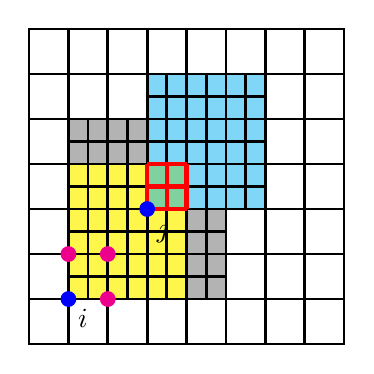
\begin{tikzpicture}[scale=4.0]
    % Define layers
    \pgfdeclarelayer{background}
    \pgfsetlayers{background,main}
    
    \coordinate (v1_1) at (0.0, 0.0);
    \coordinate (v1_2) at (0.125, 0.0);
    \coordinate (v1_3) at (0.125, 0.14285714285714285);
    \coordinate (v1_4) at (0.0, 0.14285714285714285);
    \draw[black, line width=1.0pt] (v1_1) -- (v1_2) -- (v1_3) -- (v1_4) -- cycle;
    \coordinate (v2_1) at (0.125, 0.0);
    \coordinate (v2_2) at (0.25, 0.0);
    \coordinate (v2_3) at (0.25, 0.14285714285714285);
    \coordinate (v2_4) at (0.125, 0.14285714285714285);
    \draw[black, line width=1.0pt] (v2_1) -- (v2_2) -- (v2_3) -- (v2_4) -- cycle;
    \coordinate (v3_1) at (0.25, 0.0);
    \coordinate (v3_2) at (0.375, 0.0);
    \coordinate (v3_3) at (0.375, 0.14285714285714285);
    \coordinate (v3_4) at (0.25, 0.14285714285714285);
    \draw[black, line width=1.0pt] (v3_1) -- (v3_2) -- (v3_3) -- (v3_4) -- cycle;
    \coordinate (v4_1) at (0.375, 0.0);
    \coordinate (v4_2) at (0.5, 0.0);
    \coordinate (v4_3) at (0.5, 0.14285714285714285);
    \coordinate (v4_4) at (0.375, 0.14285714285714285);
    \draw[black, line width=1.0pt] (v4_1) -- (v4_2) -- (v4_3) -- (v4_4) -- cycle;
    \coordinate (v5_1) at (0.5, 0.0);
    \coordinate (v5_2) at (0.625, 0.0);
    \coordinate (v5_3) at (0.625, 0.14285714285714285);
    \coordinate (v5_4) at (0.5, 0.14285714285714285);
    \draw[black, line width=1.0pt] (v5_1) -- (v5_2) -- (v5_3) -- (v5_4) -- cycle;
    \coordinate (v6_1) at (0.625, 0.0);
    \coordinate (v6_2) at (0.75, 0.0);
    \coordinate (v6_3) at (0.75, 0.14285714285714285);
    \coordinate (v6_4) at (0.625, 0.14285714285714285);
    \draw[black, line width=1.0pt] (v6_1) -- (v6_2) -- (v6_3) -- (v6_4) -- cycle;
    \coordinate (v7_1) at (0.75, 0.0);
    \coordinate (v7_2) at (0.875, 0.0);
    \coordinate (v7_3) at (0.875, 0.14285714285714285);
    \coordinate (v7_4) at (0.75, 0.14285714285714285);
    \draw[black, line width=1.0pt] (v7_1) -- (v7_2) -- (v7_3) -- (v7_4) -- cycle;
    \coordinate (v8_1) at (0.875, 0.0);
    \coordinate (v8_2) at (1.0, 0.0);
    \coordinate (v8_3) at (1.0, 0.14285714285714285);
    \coordinate (v8_4) at (0.875, 0.14285714285714285);
    \draw[black, line width=1.0pt] (v8_1) -- (v8_2) -- (v8_3) -- (v8_4) -- cycle;
    \coordinate (v9_1) at (0.0, 0.14285714285714285);
    \coordinate (v9_2) at (0.125, 0.14285714285714285);
    \coordinate (v9_3) at (0.125, 0.2857142857142857);
    \coordinate (v9_4) at (0.0, 0.2857142857142857);
    \draw[black, line width=1.0pt] (v9_1) -- (v9_2) -- (v9_3) -- (v9_4) -- cycle;
    \coordinate (v10_1) at (0.625, 0.14285714285714285);
    \coordinate (v10_2) at (0.75, 0.14285714285714285);
    \coordinate (v10_3) at (0.75, 0.2857142857142857);
    \coordinate (v10_4) at (0.625, 0.2857142857142857);
    \draw[black, line width=1.0pt] (v10_1) -- (v10_2) -- (v10_3) -- (v10_4) -- cycle;
    \coordinate (v11_1) at (0.75, 0.14285714285714285);
    \coordinate (v11_2) at (0.875, 0.14285714285714285);
    \coordinate (v11_3) at (0.875, 0.2857142857142857);
    \coordinate (v11_4) at (0.75, 0.2857142857142857);
    \draw[black, line width=1.0pt] (v11_1) -- (v11_2) -- (v11_3) -- (v11_4) -- cycle;
    \coordinate (v12_1) at (0.875, 0.14285714285714285);
    \coordinate (v12_2) at (1.0, 0.14285714285714285);
    \coordinate (v12_3) at (1.0, 0.2857142857142857);
    \coordinate (v12_4) at (0.875, 0.2857142857142857);
    \draw[black, line width=1.0pt] (v12_1) -- (v12_2) -- (v12_3) -- (v12_4) -- cycle;
    \coordinate (v13_1) at (0.0, 0.2857142857142857);
    \coordinate (v13_2) at (0.125, 0.2857142857142857);
    \coordinate (v13_3) at (0.125, 0.42857142857142855);
    \coordinate (v13_4) at (0.0, 0.42857142857142855);
    \draw[black, line width=1.0pt] (v13_1) -- (v13_2) -- (v13_3) -- (v13_4) -- cycle;
    \coordinate (v14_1) at (0.625, 0.2857142857142857);
    \coordinate (v14_2) at (0.75, 0.2857142857142857);
    \coordinate (v14_3) at (0.75, 0.42857142857142855);
    \coordinate (v14_4) at (0.625, 0.42857142857142855);
    \draw[black, line width=1.0pt] (v14_1) -- (v14_2) -- (v14_3) -- (v14_4) -- cycle;
    \coordinate (v15_1) at (0.75, 0.2857142857142857);
    \coordinate (v15_2) at (0.875, 0.2857142857142857);
    \coordinate (v15_3) at (0.875, 0.42857142857142855);
    \coordinate (v15_4) at (0.75, 0.42857142857142855);
    \draw[black, line width=1.0pt] (v15_1) -- (v15_2) -- (v15_3) -- (v15_4) -- cycle;
    \coordinate (v16_1) at (0.875, 0.2857142857142857);
    \coordinate (v16_2) at (1.0, 0.2857142857142857);
    \coordinate (v16_3) at (1.0, 0.42857142857142855);
    \coordinate (v16_4) at (0.875, 0.42857142857142855);
    \draw[black, line width=1.0pt] (v16_1) -- (v16_2) -- (v16_3) -- (v16_4) -- cycle;
    \coordinate (v17_1) at (0.0, 0.42857142857142855);
    \coordinate (v17_2) at (0.125, 0.42857142857142855);
    \coordinate (v17_3) at (0.125, 0.5714285714285714);
    \coordinate (v17_4) at (0.0, 0.5714285714285714);
    \draw[black, line width=1.0pt] (v17_1) -- (v17_2) -- (v17_3) -- (v17_4) -- cycle;
    \coordinate (v18_1) at (0.75, 0.42857142857142855);
    \coordinate (v18_2) at (0.875, 0.42857142857142855);
    \coordinate (v18_3) at (0.875, 0.5714285714285714);
    \coordinate (v18_4) at (0.75, 0.5714285714285714);
    \draw[black, line width=1.0pt] (v18_1) -- (v18_2) -- (v18_3) -- (v18_4) -- cycle;
    \coordinate (v19_1) at (0.875, 0.42857142857142855);
    \coordinate (v19_2) at (1.0, 0.42857142857142855);
    \coordinate (v19_3) at (1.0, 0.5714285714285714);
    \coordinate (v19_4) at (0.875, 0.5714285714285714);
    \draw[black, line width=1.0pt] (v19_1) -- (v19_2) -- (v19_3) -- (v19_4) -- cycle;
    \coordinate (v20_1) at (0.0, 0.5714285714285714);
    \coordinate (v20_2) at (0.125, 0.5714285714285714);
    \coordinate (v20_3) at (0.125, 0.7142857142857143);
    \coordinate (v20_4) at (0.0, 0.7142857142857143);
    \draw[black, line width=1.0pt] (v20_1) -- (v20_2) -- (v20_3) -- (v20_4) -- cycle;
    \coordinate (v21_1) at (0.75, 0.5714285714285714);
    \coordinate (v21_2) at (0.875, 0.5714285714285714);
    \coordinate (v21_3) at (0.875, 0.7142857142857143);
    \coordinate (v21_4) at (0.75, 0.7142857142857143);
    \draw[black, line width=1.0pt] (v21_1) -- (v21_2) -- (v21_3) -- (v21_4) -- cycle;
    \coordinate (v22_1) at (0.875, 0.5714285714285714);
    \coordinate (v22_2) at (1.0, 0.5714285714285714);
    \coordinate (v22_3) at (1.0, 0.7142857142857143);
    \coordinate (v22_4) at (0.875, 0.7142857142857143);
    \draw[black, line width=1.0pt] (v22_1) -- (v22_2) -- (v22_3) -- (v22_4) -- cycle;
    \coordinate (v23_1) at (0.0, 0.7142857142857143);
    \coordinate (v23_2) at (0.125, 0.7142857142857143);
    \coordinate (v23_3) at (0.125, 0.8571428571428571);
    \coordinate (v23_4) at (0.0, 0.8571428571428571);
    \draw[black, line width=1.0pt] (v23_1) -- (v23_2) -- (v23_3) -- (v23_4) -- cycle;
    \coordinate (v24_1) at (0.125, 0.7142857142857143);
    \coordinate (v24_2) at (0.25, 0.7142857142857143);
    \coordinate (v24_3) at (0.25, 0.8571428571428571);
    \coordinate (v24_4) at (0.125, 0.8571428571428571);
    \draw[black, line width=1.0pt] (v24_1) -- (v24_2) -- (v24_3) -- (v24_4) -- cycle;
    \coordinate (v25_1) at (0.25, 0.7142857142857143);
    \coordinate (v25_2) at (0.375, 0.7142857142857143);
    \coordinate (v25_3) at (0.375, 0.8571428571428571);
    \coordinate (v25_4) at (0.25, 0.8571428571428571);
    \draw[black, line width=1.0pt] (v25_1) -- (v25_2) -- (v25_3) -- (v25_4) -- cycle;
    \coordinate (v26_1) at (0.75, 0.7142857142857143);
    \coordinate (v26_2) at (0.875, 0.7142857142857143);
    \coordinate (v26_3) at (0.875, 0.8571428571428571);
    \coordinate (v26_4) at (0.75, 0.8571428571428571);
    \draw[black, line width=1.0pt] (v26_1) -- (v26_2) -- (v26_3) -- (v26_4) -- cycle;
    \coordinate (v27_1) at (0.875, 0.7142857142857143);
    \coordinate (v27_2) at (1.0, 0.7142857142857143);
    \coordinate (v27_3) at (1.0, 0.8571428571428571);
    \coordinate (v27_4) at (0.875, 0.8571428571428571);
    \draw[black, line width=1.0pt] (v27_1) -- (v27_2) -- (v27_3) -- (v27_4) -- cycle;
    \coordinate (v28_1) at (0.0, 0.8571428571428571);
    \coordinate (v28_2) at (0.125, 0.8571428571428571);
    \coordinate (v28_3) at (0.125, 1.0);
    \coordinate (v28_4) at (0.0, 1.0);
    \draw[black, line width=1.0pt] (v28_1) -- (v28_2) -- (v28_3) -- (v28_4) -- cycle;
    \coordinate (v29_1) at (0.125, 0.8571428571428571);
    \coordinate (v29_2) at (0.25, 0.8571428571428571);
    \coordinate (v29_3) at (0.25, 1.0);
    \coordinate (v29_4) at (0.125, 1.0);
    \draw[black, line width=1.0pt] (v29_1) -- (v29_2) -- (v29_3) -- (v29_4) -- cycle;
    \coordinate (v30_1) at (0.25, 0.8571428571428571);
    \coordinate (v30_2) at (0.375, 0.8571428571428571);
    \coordinate (v30_3) at (0.375, 1.0);
    \coordinate (v30_4) at (0.25, 1.0);
    \draw[black, line width=1.0pt] (v30_1) -- (v30_2) -- (v30_3) -- (v30_4) -- cycle;
    \coordinate (v31_1) at (0.375, 0.8571428571428571);
    \coordinate (v31_2) at (0.5, 0.8571428571428571);
    \coordinate (v31_3) at (0.5, 1.0);
    \coordinate (v31_4) at (0.375, 1.0);
    \draw[black, line width=1.0pt] (v31_1) -- (v31_2) -- (v31_3) -- (v31_4) -- cycle;
    \coordinate (v32_1) at (0.5, 0.8571428571428571);
    \coordinate (v32_2) at (0.625, 0.8571428571428571);
    \coordinate (v32_3) at (0.625, 1.0);
    \coordinate (v32_4) at (0.5, 1.0);
    \draw[black, line width=1.0pt] (v32_1) -- (v32_2) -- (v32_3) -- (v32_4) -- cycle;
    \coordinate (v33_1) at (0.625, 0.8571428571428571);
    \coordinate (v33_2) at (0.75, 0.8571428571428571);
    \coordinate (v33_3) at (0.75, 1.0);
    \coordinate (v33_4) at (0.625, 1.0);
    \draw[black, line width=1.0pt] (v33_1) -- (v33_2) -- (v33_3) -- (v33_4) -- cycle;
    \coordinate (v34_1) at (0.75, 0.8571428571428571);
    \coordinate (v34_2) at (0.875, 0.8571428571428571);
    \coordinate (v34_3) at (0.875, 1.0);
    \coordinate (v34_4) at (0.75, 1.0);
    \draw[black, line width=1.0pt] (v34_1) -- (v34_2) -- (v34_3) -- (v34_4) -- cycle;
    \coordinate (v35_1) at (0.875, 0.8571428571428571);
    \coordinate (v35_2) at (1.0, 0.8571428571428571);
    \coordinate (v35_3) at (1.0, 1.0);
    \coordinate (v35_4) at (0.875, 1.0);
    \draw[black, line width=1.0pt] (v35_1) -- (v35_2) -- (v35_3) -- (v35_4) -- cycle;
    \coordinate (v36_1) at (0.125, 0.14285714285714285);
    \coordinate (v36_2) at (0.1875, 0.14285714285714285);
    \coordinate (v36_3) at (0.1875, 0.21428571428571427);
    \coordinate (v36_4) at (0.125, 0.21428571428571427);
    \draw[black, line width=1.0pt] (v36_1) -- (v36_2) -- (v36_3) -- (v36_4) -- cycle;
    \coordinate (v37_1) at (0.1875, 0.14285714285714285);
    \coordinate (v37_2) at (0.25, 0.14285714285714285);
    \coordinate (v37_3) at (0.25, 0.21428571428571427);
    \coordinate (v37_4) at (0.1875, 0.21428571428571427);
    \draw[black, line width=1.0pt] (v37_1) -- (v37_2) -- (v37_3) -- (v37_4) -- cycle;
    \coordinate (v38_1) at (0.25, 0.14285714285714285);
    \coordinate (v38_2) at (0.3125, 0.14285714285714285);
    \coordinate (v38_3) at (0.3125, 0.21428571428571427);
    \coordinate (v38_4) at (0.25, 0.21428571428571427);
    \draw[black, line width=1.0pt] (v38_1) -- (v38_2) -- (v38_3) -- (v38_4) -- cycle;
    \coordinate (v39_1) at (0.3125, 0.14285714285714285);
    \coordinate (v39_2) at (0.375, 0.14285714285714285);
    \coordinate (v39_3) at (0.375, 0.21428571428571427);
    \coordinate (v39_4) at (0.3125, 0.21428571428571427);
    \draw[black, line width=1.0pt] (v39_1) -- (v39_2) -- (v39_3) -- (v39_4) -- cycle;
    \coordinate (v40_1) at (0.375, 0.14285714285714285);
    \coordinate (v40_2) at (0.4375, 0.14285714285714285);
    \coordinate (v40_3) at (0.4375, 0.21428571428571427);
    \coordinate (v40_4) at (0.375, 0.21428571428571427);
    \draw[black, line width=1.0pt] (v40_1) -- (v40_2) -- (v40_3) -- (v40_4) -- cycle;
    \coordinate (v41_1) at (0.4375, 0.14285714285714285);
    \coordinate (v41_2) at (0.5, 0.14285714285714285);
    \coordinate (v41_3) at (0.5, 0.21428571428571427);
    \coordinate (v41_4) at (0.4375, 0.21428571428571427);
    \draw[black, line width=1.0pt] (v41_1) -- (v41_2) -- (v41_3) -- (v41_4) -- cycle;
    \coordinate (v42_1) at (0.5, 0.14285714285714285);
    \coordinate (v42_2) at (0.5625, 0.14285714285714285);
    \coordinate (v42_3) at (0.5625, 0.21428571428571427);
    \coordinate (v42_4) at (0.5, 0.21428571428571427);
    \draw[black, line width=1.0pt] (v42_1) -- (v42_2) -- (v42_3) -- (v42_4) -- cycle;
    \coordinate (v43_1) at (0.5625, 0.14285714285714285);
    \coordinate (v43_2) at (0.625, 0.14285714285714285);
    \coordinate (v43_3) at (0.625, 0.21428571428571427);
    \coordinate (v43_4) at (0.5625, 0.21428571428571427);
    \draw[black, line width=1.0pt] (v43_1) -- (v43_2) -- (v43_3) -- (v43_4) -- cycle;
    \coordinate (v44_1) at (0.125, 0.21428571428571427);
    \coordinate (v44_2) at (0.1875, 0.21428571428571427);
    \coordinate (v44_3) at (0.1875, 0.2857142857142857);
    \coordinate (v44_4) at (0.125, 0.2857142857142857);
    \draw[black, line width=1.0pt] (v44_1) -- (v44_2) -- (v44_3) -- (v44_4) -- cycle;
    \coordinate (v45_1) at (0.1875, 0.21428571428571427);
    \coordinate (v45_2) at (0.25, 0.21428571428571427);
    \coordinate (v45_3) at (0.25, 0.2857142857142857);
    \coordinate (v45_4) at (0.1875, 0.2857142857142857);
    \draw[black, line width=1.0pt] (v45_1) -- (v45_2) -- (v45_3) -- (v45_4) -- cycle;
    \coordinate (v46_1) at (0.25, 0.21428571428571427);
    \coordinate (v46_2) at (0.3125, 0.21428571428571427);
    \coordinate (v46_3) at (0.3125, 0.2857142857142857);
    \coordinate (v46_4) at (0.25, 0.2857142857142857);
    \draw[black, line width=1.0pt] (v46_1) -- (v46_2) -- (v46_3) -- (v46_4) -- cycle;
    \coordinate (v47_1) at (0.3125, 0.21428571428571427);
    \coordinate (v47_2) at (0.375, 0.21428571428571427);
    \coordinate (v47_3) at (0.375, 0.2857142857142857);
    \coordinate (v47_4) at (0.3125, 0.2857142857142857);
    \draw[black, line width=1.0pt] (v47_1) -- (v47_2) -- (v47_3) -- (v47_4) -- cycle;
    \coordinate (v48_1) at (0.375, 0.21428571428571427);
    \coordinate (v48_2) at (0.4375, 0.21428571428571427);
    \coordinate (v48_3) at (0.4375, 0.2857142857142857);
    \coordinate (v48_4) at (0.375, 0.2857142857142857);
    \draw[black, line width=1.0pt] (v48_1) -- (v48_2) -- (v48_3) -- (v48_4) -- cycle;
    \coordinate (v49_1) at (0.4375, 0.21428571428571427);
    \coordinate (v49_2) at (0.5, 0.21428571428571427);
    \coordinate (v49_3) at (0.5, 0.2857142857142857);
    \coordinate (v49_4) at (0.4375, 0.2857142857142857);
    \draw[black, line width=1.0pt] (v49_1) -- (v49_2) -- (v49_3) -- (v49_4) -- cycle;
    \coordinate (v50_1) at (0.5, 0.21428571428571427);
    \coordinate (v50_2) at (0.5625, 0.21428571428571427);
    \coordinate (v50_3) at (0.5625, 0.2857142857142857);
    \coordinate (v50_4) at (0.5, 0.2857142857142857);
    \draw[black, line width=1.0pt] (v50_1) -- (v50_2) -- (v50_3) -- (v50_4) -- cycle;
    \coordinate (v51_1) at (0.5625, 0.21428571428571427);
    \coordinate (v51_2) at (0.625, 0.21428571428571427);
    \coordinate (v51_3) at (0.625, 0.2857142857142857);
    \coordinate (v51_4) at (0.5625, 0.2857142857142857);
    \draw[black, line width=1.0pt] (v51_1) -- (v51_2) -- (v51_3) -- (v51_4) -- cycle;
    \coordinate (v52_1) at (0.125, 0.2857142857142857);
    \coordinate (v52_2) at (0.1875, 0.2857142857142857);
    \coordinate (v52_3) at (0.1875, 0.3571428571428571);
    \coordinate (v52_4) at (0.125, 0.3571428571428571);
    \draw[black, line width=1.0pt] (v52_1) -- (v52_2) -- (v52_3) -- (v52_4) -- cycle;
    \coordinate (v53_1) at (0.1875, 0.2857142857142857);
    \coordinate (v53_2) at (0.25, 0.2857142857142857);
    \coordinate (v53_3) at (0.25, 0.3571428571428571);
    \coordinate (v53_4) at (0.1875, 0.3571428571428571);
    \draw[black, line width=1.0pt] (v53_1) -- (v53_2) -- (v53_3) -- (v53_4) -- cycle;
    \coordinate (v54_1) at (0.25, 0.2857142857142857);
    \coordinate (v54_2) at (0.3125, 0.2857142857142857);
    \coordinate (v54_3) at (0.3125, 0.3571428571428571);
    \coordinate (v54_4) at (0.25, 0.3571428571428571);
    \draw[black, line width=1.0pt] (v54_1) -- (v54_2) -- (v54_3) -- (v54_4) -- cycle;
    \coordinate (v55_1) at (0.3125, 0.2857142857142857);
    \coordinate (v55_2) at (0.375, 0.2857142857142857);
    \coordinate (v55_3) at (0.375, 0.3571428571428571);
    \coordinate (v55_4) at (0.3125, 0.3571428571428571);
    \draw[black, line width=1.0pt] (v55_1) -- (v55_2) -- (v55_3) -- (v55_4) -- cycle;
    \coordinate (v56_1) at (0.375, 0.2857142857142857);
    \coordinate (v56_2) at (0.4375, 0.2857142857142857);
    \coordinate (v56_3) at (0.4375, 0.3571428571428571);
    \coordinate (v56_4) at (0.375, 0.3571428571428571);
    \draw[black, line width=1.0pt] (v56_1) -- (v56_2) -- (v56_3) -- (v56_4) -- cycle;
    \coordinate (v57_1) at (0.4375, 0.2857142857142857);
    \coordinate (v57_2) at (0.5, 0.2857142857142857);
    \coordinate (v57_3) at (0.5, 0.3571428571428571);
    \coordinate (v57_4) at (0.4375, 0.3571428571428571);
    \draw[black, line width=1.0pt] (v57_1) -- (v57_2) -- (v57_3) -- (v57_4) -- cycle;
    \coordinate (v58_1) at (0.5, 0.2857142857142857);
    \coordinate (v58_2) at (0.5625, 0.2857142857142857);
    \coordinate (v58_3) at (0.5625, 0.3571428571428571);
    \coordinate (v58_4) at (0.5, 0.3571428571428571);
    \draw[black, line width=1.0pt] (v58_1) -- (v58_2) -- (v58_3) -- (v58_4) -- cycle;
    \coordinate (v59_1) at (0.5625, 0.2857142857142857);
    \coordinate (v59_2) at (0.625, 0.2857142857142857);
    \coordinate (v59_3) at (0.625, 0.3571428571428571);
    \coordinate (v59_4) at (0.5625, 0.3571428571428571);
    \draw[black, line width=1.0pt] (v59_1) -- (v59_2) -- (v59_3) -- (v59_4) -- cycle;
    \coordinate (v60_1) at (0.125, 0.3571428571428571);
    \coordinate (v60_2) at (0.1875, 0.3571428571428571);
    \coordinate (v60_3) at (0.1875, 0.42857142857142855);
    \coordinate (v60_4) at (0.125, 0.42857142857142855);
    \draw[black, line width=1.0pt] (v60_1) -- (v60_2) -- (v60_3) -- (v60_4) -- cycle;
    \coordinate (v61_1) at (0.1875, 0.3571428571428571);
    \coordinate (v61_2) at (0.25, 0.3571428571428571);
    \coordinate (v61_3) at (0.25, 0.42857142857142855);
    \coordinate (v61_4) at (0.1875, 0.42857142857142855);
    \draw[black, line width=1.0pt] (v61_1) -- (v61_2) -- (v61_3) -- (v61_4) -- cycle;
    \coordinate (v62_1) at (0.25, 0.3571428571428571);
    \coordinate (v62_2) at (0.3125, 0.3571428571428571);
    \coordinate (v62_3) at (0.3125, 0.42857142857142855);
    \coordinate (v62_4) at (0.25, 0.42857142857142855);
    \draw[black, line width=1.0pt] (v62_1) -- (v62_2) -- (v62_3) -- (v62_4) -- cycle;
    \coordinate (v63_1) at (0.3125, 0.3571428571428571);
    \coordinate (v63_2) at (0.375, 0.3571428571428571);
    \coordinate (v63_3) at (0.375, 0.42857142857142855);
    \coordinate (v63_4) at (0.3125, 0.42857142857142855);
    \draw[black, line width=1.0pt] (v63_1) -- (v63_2) -- (v63_3) -- (v63_4) -- cycle;
    \coordinate (v64_1) at (0.375, 0.3571428571428571);
    \coordinate (v64_2) at (0.4375, 0.3571428571428571);
    \coordinate (v64_3) at (0.4375, 0.42857142857142855);
    \coordinate (v64_4) at (0.375, 0.42857142857142855);
    \draw[black, line width=1.0pt] (v64_1) -- (v64_2) -- (v64_3) -- (v64_4) -- cycle;
    \coordinate (v65_1) at (0.4375, 0.3571428571428571);
    \coordinate (v65_2) at (0.5, 0.3571428571428571);
    \coordinate (v65_3) at (0.5, 0.42857142857142855);
    \coordinate (v65_4) at (0.4375, 0.42857142857142855);
    \draw[black, line width=1.0pt] (v65_1) -- (v65_2) -- (v65_3) -- (v65_4) -- cycle;
    \coordinate (v66_1) at (0.5, 0.3571428571428571);
    \coordinate (v66_2) at (0.5625, 0.3571428571428571);
    \coordinate (v66_3) at (0.5625, 0.42857142857142855);
    \coordinate (v66_4) at (0.5, 0.42857142857142855);
    \draw[black, line width=1.0pt] (v66_1) -- (v66_2) -- (v66_3) -- (v66_4) -- cycle;
    \coordinate (v67_1) at (0.5625, 0.3571428571428571);
    \coordinate (v67_2) at (0.625, 0.3571428571428571);
    \coordinate (v67_3) at (0.625, 0.42857142857142855);
    \coordinate (v67_4) at (0.5625, 0.42857142857142855);
    \draw[black, line width=1.0pt] (v67_1) -- (v67_2) -- (v67_3) -- (v67_4) -- cycle;
    \coordinate (v68_1) at (0.125, 0.42857142857142855);
    \coordinate (v68_2) at (0.1875, 0.42857142857142855);
    \coordinate (v68_3) at (0.1875, 0.5);
    \coordinate (v68_4) at (0.125, 0.5);
    \draw[black, line width=1.0pt] (v68_1) -- (v68_2) -- (v68_3) -- (v68_4) -- cycle;
    \coordinate (v69_1) at (0.1875, 0.42857142857142855);
    \coordinate (v69_2) at (0.25, 0.42857142857142855);
    \coordinate (v69_3) at (0.25, 0.5);
    \coordinate (v69_4) at (0.1875, 0.5);
    \draw[black, line width=1.0pt] (v69_1) -- (v69_2) -- (v69_3) -- (v69_4) -- cycle;
    \coordinate (v70_1) at (0.25, 0.42857142857142855);
    \coordinate (v70_2) at (0.3125, 0.42857142857142855);
    \coordinate (v70_3) at (0.3125, 0.5);
    \coordinate (v70_4) at (0.25, 0.5);
    \draw[black, line width=1.0pt] (v70_1) -- (v70_2) -- (v70_3) -- (v70_4) -- cycle;
    \coordinate (v71_1) at (0.3125, 0.42857142857142855);
    \coordinate (v71_2) at (0.375, 0.42857142857142855);
    \coordinate (v71_3) at (0.375, 0.5);
    \coordinate (v71_4) at (0.3125, 0.5);
    \draw[black, line width=1.0pt] (v71_1) -- (v71_2) -- (v71_3) -- (v71_4) -- cycle;
    \coordinate (v72_1) at (0.375, 0.42857142857142855);
    \coordinate (v72_2) at (0.4375, 0.42857142857142855);
    \coordinate (v72_3) at (0.4375, 0.5);
    \coordinate (v72_4) at (0.375, 0.5);
    \draw[black, line width=1.0pt] (v72_1) -- (v72_2) -- (v72_3) -- (v72_4) -- cycle;
    \coordinate (v73_1) at (0.4375, 0.42857142857142855);
    \coordinate (v73_2) at (0.5, 0.42857142857142855);
    \coordinate (v73_3) at (0.5, 0.5);
    \coordinate (v73_4) at (0.4375, 0.5);
    \draw[black, line width=1.0pt] (v73_1) -- (v73_2) -- (v73_3) -- (v73_4) -- cycle;
    \coordinate (v74_1) at (0.5, 0.42857142857142855);
    \coordinate (v74_2) at (0.5625, 0.42857142857142855);
    \coordinate (v74_3) at (0.5625, 0.5);
    \coordinate (v74_4) at (0.5, 0.5);
    \draw[black, line width=1.0pt] (v74_1) -- (v74_2) -- (v74_3) -- (v74_4) -- cycle;
    \coordinate (v75_1) at (0.5625, 0.42857142857142855);
    \coordinate (v75_2) at (0.625, 0.42857142857142855);
    \coordinate (v75_3) at (0.625, 0.5);
    \coordinate (v75_4) at (0.5625, 0.5);
    \draw[black, line width=1.0pt] (v75_1) -- (v75_2) -- (v75_3) -- (v75_4) -- cycle;
    \coordinate (v76_1) at (0.625, 0.42857142857142855);
    \coordinate (v76_2) at (0.6875, 0.42857142857142855);
    \coordinate (v76_3) at (0.6875, 0.5);
    \coordinate (v76_4) at (0.625, 0.5);
    \draw[black, line width=1.0pt] (v76_1) -- (v76_2) -- (v76_3) -- (v76_4) -- cycle;
    \coordinate (v77_1) at (0.6875, 0.42857142857142855);
    \coordinate (v77_2) at (0.75, 0.42857142857142855);
    \coordinate (v77_3) at (0.75, 0.5);
    \coordinate (v77_4) at (0.6875, 0.5);
    \draw[black, line width=1.0pt] (v77_1) -- (v77_2) -- (v77_3) -- (v77_4) -- cycle;
    \coordinate (v78_1) at (0.125, 0.5);
    \coordinate (v78_2) at (0.1875, 0.5);
    \coordinate (v78_3) at (0.1875, 0.5714285714285714);
    \coordinate (v78_4) at (0.125, 0.5714285714285714);
    \draw[black, line width=1.0pt] (v78_1) -- (v78_2) -- (v78_3) -- (v78_4) -- cycle;
    \coordinate (v79_1) at (0.1875, 0.5);
    \coordinate (v79_2) at (0.25, 0.5);
    \coordinate (v79_3) at (0.25, 0.5714285714285714);
    \coordinate (v79_4) at (0.1875, 0.5714285714285714);
    \draw[black, line width=1.0pt] (v79_1) -- (v79_2) -- (v79_3) -- (v79_4) -- cycle;
    \coordinate (v80_1) at (0.25, 0.5);
    \coordinate (v80_2) at (0.3125, 0.5);
    \coordinate (v80_3) at (0.3125, 0.5714285714285714);
    \coordinate (v80_4) at (0.25, 0.5714285714285714);
    \draw[black, line width=1.0pt] (v80_1) -- (v80_2) -- (v80_3) -- (v80_4) -- cycle;
    \coordinate (v81_1) at (0.3125, 0.5);
    \coordinate (v81_2) at (0.375, 0.5);
    \coordinate (v81_3) at (0.375, 0.5714285714285714);
    \coordinate (v81_4) at (0.3125, 0.5714285714285714);
    \draw[black, line width=1.0pt] (v81_1) -- (v81_2) -- (v81_3) -- (v81_4) -- cycle;
    \coordinate (v82_1) at (0.375, 0.5);
    \coordinate (v82_2) at (0.4375, 0.5);
    \coordinate (v82_3) at (0.4375, 0.5714285714285714);
    \coordinate (v82_4) at (0.375, 0.5714285714285714);
    \draw[black, line width=1.0pt] (v82_1) -- (v82_2) -- (v82_3) -- (v82_4) -- cycle;
    \coordinate (v83_1) at (0.4375, 0.5);
    \coordinate (v83_2) at (0.5, 0.5);
    \coordinate (v83_3) at (0.5, 0.5714285714285714);
    \coordinate (v83_4) at (0.4375, 0.5714285714285714);
    \draw[black, line width=1.0pt] (v83_1) -- (v83_2) -- (v83_3) -- (v83_4) -- cycle;
    \coordinate (v84_1) at (0.5, 0.5);
    \coordinate (v84_2) at (0.5625, 0.5);
    \coordinate (v84_3) at (0.5625, 0.5714285714285714);
    \coordinate (v84_4) at (0.5, 0.5714285714285714);
    \draw[black, line width=1.0pt] (v84_1) -- (v84_2) -- (v84_3) -- (v84_4) -- cycle;
    \coordinate (v85_1) at (0.5625, 0.5);
    \coordinate (v85_2) at (0.625, 0.5);
    \coordinate (v85_3) at (0.625, 0.5714285714285714);
    \coordinate (v85_4) at (0.5625, 0.5714285714285714);
    \draw[black, line width=1.0pt] (v85_1) -- (v85_2) -- (v85_3) -- (v85_4) -- cycle;
    \coordinate (v86_1) at (0.625, 0.5);
    \coordinate (v86_2) at (0.6875, 0.5);
    \coordinate (v86_3) at (0.6875, 0.5714285714285714);
    \coordinate (v86_4) at (0.625, 0.5714285714285714);
    \draw[black, line width=1.0pt] (v86_1) -- (v86_2) -- (v86_3) -- (v86_4) -- cycle;
    \coordinate (v87_1) at (0.6875, 0.5);
    \coordinate (v87_2) at (0.75, 0.5);
    \coordinate (v87_3) at (0.75, 0.5714285714285714);
    \coordinate (v87_4) at (0.6875, 0.5714285714285714);
    \draw[black, line width=1.0pt] (v87_1) -- (v87_2) -- (v87_3) -- (v87_4) -- cycle;
    \coordinate (v88_1) at (0.125, 0.5714285714285714);
    \coordinate (v88_2) at (0.1875, 0.5714285714285714);
    \coordinate (v88_3) at (0.1875, 0.6428571428571428);
    \coordinate (v88_4) at (0.125, 0.6428571428571428);
    \draw[black, line width=1.0pt] (v88_1) -- (v88_2) -- (v88_3) -- (v88_4) -- cycle;
    \coordinate (v89_1) at (0.1875, 0.5714285714285714);
    \coordinate (v89_2) at (0.25, 0.5714285714285714);
    \coordinate (v89_3) at (0.25, 0.6428571428571428);
    \coordinate (v89_4) at (0.1875, 0.6428571428571428);
    \draw[black, line width=1.0pt] (v89_1) -- (v89_2) -- (v89_3) -- (v89_4) -- cycle;
    \coordinate (v90_1) at (0.25, 0.5714285714285714);
    \coordinate (v90_2) at (0.3125, 0.5714285714285714);
    \coordinate (v90_3) at (0.3125, 0.6428571428571428);
    \coordinate (v90_4) at (0.25, 0.6428571428571428);
    \draw[black, line width=1.0pt] (v90_1) -- (v90_2) -- (v90_3) -- (v90_4) -- cycle;
    \coordinate (v91_1) at (0.3125, 0.5714285714285714);
    \coordinate (v91_2) at (0.375, 0.5714285714285714);
    \coordinate (v91_3) at (0.375, 0.6428571428571428);
    \coordinate (v91_4) at (0.3125, 0.6428571428571428);
    \draw[black, line width=1.0pt] (v91_1) -- (v91_2) -- (v91_3) -- (v91_4) -- cycle;
    \coordinate (v92_1) at (0.375, 0.5714285714285714);
    \coordinate (v92_2) at (0.4375, 0.5714285714285714);
    \coordinate (v92_3) at (0.4375, 0.6428571428571428);
    \coordinate (v92_4) at (0.375, 0.6428571428571428);
    \draw[black, line width=1.0pt] (v92_1) -- (v92_2) -- (v92_3) -- (v92_4) -- cycle;
    \coordinate (v93_1) at (0.4375, 0.5714285714285714);
    \coordinate (v93_2) at (0.5, 0.5714285714285714);
    \coordinate (v93_3) at (0.5, 0.6428571428571428);
    \coordinate (v93_4) at (0.4375, 0.6428571428571428);
    \draw[black, line width=1.0pt] (v93_1) -- (v93_2) -- (v93_3) -- (v93_4) -- cycle;
    \coordinate (v94_1) at (0.5, 0.5714285714285714);
    \coordinate (v94_2) at (0.5625, 0.5714285714285714);
    \coordinate (v94_3) at (0.5625, 0.6428571428571428);
    \coordinate (v94_4) at (0.5, 0.6428571428571428);
    \draw[black, line width=1.0pt] (v94_1) -- (v94_2) -- (v94_3) -- (v94_4) -- cycle;
    \coordinate (v95_1) at (0.5625, 0.5714285714285714);
    \coordinate (v95_2) at (0.625, 0.5714285714285714);
    \coordinate (v95_3) at (0.625, 0.6428571428571428);
    \coordinate (v95_4) at (0.5625, 0.6428571428571428);
    \draw[black, line width=1.0pt] (v95_1) -- (v95_2) -- (v95_3) -- (v95_4) -- cycle;
    \coordinate (v96_1) at (0.625, 0.5714285714285714);
    \coordinate (v96_2) at (0.6875, 0.5714285714285714);
    \coordinate (v96_3) at (0.6875, 0.6428571428571428);
    \coordinate (v96_4) at (0.625, 0.6428571428571428);
    \draw[black, line width=1.0pt] (v96_1) -- (v96_2) -- (v96_3) -- (v96_4) -- cycle;
    \coordinate (v97_1) at (0.6875, 0.5714285714285714);
    \coordinate (v97_2) at (0.75, 0.5714285714285714);
    \coordinate (v97_3) at (0.75, 0.6428571428571428);
    \coordinate (v97_4) at (0.6875, 0.6428571428571428);
    \draw[black, line width=1.0pt] (v97_1) -- (v97_2) -- (v97_3) -- (v97_4) -- cycle;
    \coordinate (v98_1) at (0.125, 0.6428571428571428);
    \coordinate (v98_2) at (0.1875, 0.6428571428571428);
    \coordinate (v98_3) at (0.1875, 0.7142857142857143);
    \coordinate (v98_4) at (0.125, 0.7142857142857143);
    \draw[black, line width=1.0pt] (v98_1) -- (v98_2) -- (v98_3) -- (v98_4) -- cycle;
    \coordinate (v99_1) at (0.1875, 0.6428571428571428);
    \coordinate (v99_2) at (0.25, 0.6428571428571428);
    \coordinate (v99_3) at (0.25, 0.7142857142857143);
    \coordinate (v99_4) at (0.1875, 0.7142857142857143);
    \draw[black, line width=1.0pt] (v99_1) -- (v99_2) -- (v99_3) -- (v99_4) -- cycle;
    \coordinate (v100_1) at (0.25, 0.6428571428571428);
    \coordinate (v100_2) at (0.3125, 0.6428571428571428);
    \coordinate (v100_3) at (0.3125, 0.7142857142857143);
    \coordinate (v100_4) at (0.25, 0.7142857142857143);
    \draw[black, line width=1.0pt] (v100_1) -- (v100_2) -- (v100_3) -- (v100_4) -- cycle;
    \coordinate (v101_1) at (0.3125, 0.6428571428571428);
    \coordinate (v101_2) at (0.375, 0.6428571428571428);
    \coordinate (v101_3) at (0.375, 0.7142857142857143);
    \coordinate (v101_4) at (0.3125, 0.7142857142857143);
    \draw[black, line width=1.0pt] (v101_1) -- (v101_2) -- (v101_3) -- (v101_4) -- cycle;
    \coordinate (v102_1) at (0.375, 0.6428571428571428);
    \coordinate (v102_2) at (0.4375, 0.6428571428571428);
    \coordinate (v102_3) at (0.4375, 0.7142857142857143);
    \coordinate (v102_4) at (0.375, 0.7142857142857143);
    \draw[black, line width=1.0pt] (v102_1) -- (v102_2) -- (v102_3) -- (v102_4) -- cycle;
    \coordinate (v103_1) at (0.4375, 0.6428571428571428);
    \coordinate (v103_2) at (0.5, 0.6428571428571428);
    \coordinate (v103_3) at (0.5, 0.7142857142857143);
    \coordinate (v103_4) at (0.4375, 0.7142857142857143);
    \draw[black, line width=1.0pt] (v103_1) -- (v103_2) -- (v103_3) -- (v103_4) -- cycle;
    \coordinate (v104_1) at (0.5, 0.6428571428571428);
    \coordinate (v104_2) at (0.5625, 0.6428571428571428);
    \coordinate (v104_3) at (0.5625, 0.7142857142857143);
    \coordinate (v104_4) at (0.5, 0.7142857142857143);
    \draw[black, line width=1.0pt] (v104_1) -- (v104_2) -- (v104_3) -- (v104_4) -- cycle;
    \coordinate (v105_1) at (0.5625, 0.6428571428571428);
    \coordinate (v105_2) at (0.625, 0.6428571428571428);
    \coordinate (v105_3) at (0.625, 0.7142857142857143);
    \coordinate (v105_4) at (0.5625, 0.7142857142857143);
    \draw[black, line width=1.0pt] (v105_1) -- (v105_2) -- (v105_3) -- (v105_4) -- cycle;
    \coordinate (v106_1) at (0.625, 0.6428571428571428);
    \coordinate (v106_2) at (0.6875, 0.6428571428571428);
    \coordinate (v106_3) at (0.6875, 0.7142857142857143);
    \coordinate (v106_4) at (0.625, 0.7142857142857143);
    \draw[black, line width=1.0pt] (v106_1) -- (v106_2) -- (v106_3) -- (v106_4) -- cycle;
    \coordinate (v107_1) at (0.6875, 0.6428571428571428);
    \coordinate (v107_2) at (0.75, 0.6428571428571428);
    \coordinate (v107_3) at (0.75, 0.7142857142857143);
    \coordinate (v107_4) at (0.6875, 0.7142857142857143);
    \draw[black, line width=1.0pt] (v107_1) -- (v107_2) -- (v107_3) -- (v107_4) -- cycle;
    \coordinate (v108_1) at (0.375, 0.7142857142857143);
    \coordinate (v108_2) at (0.4375, 0.7142857142857143);
    \coordinate (v108_3) at (0.4375, 0.7857142857142857);
    \coordinate (v108_4) at (0.375, 0.7857142857142857);
    \draw[black, line width=1.0pt] (v108_1) -- (v108_2) -- (v108_3) -- (v108_4) -- cycle;
    \coordinate (v109_1) at (0.4375, 0.7142857142857143);
    \coordinate (v109_2) at (0.5, 0.7142857142857143);
    \coordinate (v109_3) at (0.5, 0.7857142857142857);
    \coordinate (v109_4) at (0.4375, 0.7857142857142857);
    \draw[black, line width=1.0pt] (v109_1) -- (v109_2) -- (v109_3) -- (v109_4) -- cycle;
    \coordinate (v110_1) at (0.5, 0.7142857142857143);
    \coordinate (v110_2) at (0.5625, 0.7142857142857143);
    \coordinate (v110_3) at (0.5625, 0.7857142857142857);
    \coordinate (v110_4) at (0.5, 0.7857142857142857);
    \draw[black, line width=1.0pt] (v110_1) -- (v110_2) -- (v110_3) -- (v110_4) -- cycle;
    \coordinate (v111_1) at (0.5625, 0.7142857142857143);
    \coordinate (v111_2) at (0.625, 0.7142857142857143);
    \coordinate (v111_3) at (0.625, 0.7857142857142857);
    \coordinate (v111_4) at (0.5625, 0.7857142857142857);
    \draw[black, line width=1.0pt] (v111_1) -- (v111_2) -- (v111_3) -- (v111_4) -- cycle;
    \coordinate (v112_1) at (0.625, 0.7142857142857143);
    \coordinate (v112_2) at (0.6875, 0.7142857142857143);
    \coordinate (v112_3) at (0.6875, 0.7857142857142857);
    \coordinate (v112_4) at (0.625, 0.7857142857142857);
    \draw[black, line width=1.0pt] (v112_1) -- (v112_2) -- (v112_3) -- (v112_4) -- cycle;
    \coordinate (v113_1) at (0.6875, 0.7142857142857143);
    \coordinate (v113_2) at (0.75, 0.7142857142857143);
    \coordinate (v113_3) at (0.75, 0.7857142857142857);
    \coordinate (v113_4) at (0.6875, 0.7857142857142857);
    \draw[black, line width=1.0pt] (v113_1) -- (v113_2) -- (v113_3) -- (v113_4) -- cycle;
    \coordinate (v114_1) at (0.375, 0.7857142857142857);
    \coordinate (v114_2) at (0.4375, 0.7857142857142857);
    \coordinate (v114_3) at (0.4375, 0.8571428571428571);
    \coordinate (v114_4) at (0.375, 0.8571428571428571);
    \draw[black, line width=1.0pt] (v114_1) -- (v114_2) -- (v114_3) -- (v114_4) -- cycle;
    \coordinate (v115_1) at (0.4375, 0.7857142857142857);
    \coordinate (v115_2) at (0.5, 0.7857142857142857);
    \coordinate (v115_3) at (0.5, 0.8571428571428571);
    \coordinate (v115_4) at (0.4375, 0.8571428571428571);
    \draw[black, line width=1.0pt] (v115_1) -- (v115_2) -- (v115_3) -- (v115_4) -- cycle;
    \coordinate (v116_1) at (0.5, 0.7857142857142857);
    \coordinate (v116_2) at (0.5625, 0.7857142857142857);
    \coordinate (v116_3) at (0.5625, 0.8571428571428571);
    \coordinate (v116_4) at (0.5, 0.8571428571428571);
    \draw[black, line width=1.0pt] (v116_1) -- (v116_2) -- (v116_3) -- (v116_4) -- cycle;
    \coordinate (v117_1) at (0.5625, 0.7857142857142857);
    \coordinate (v117_2) at (0.625, 0.7857142857142857);
    \coordinate (v117_3) at (0.625, 0.8571428571428571);
    \coordinate (v117_4) at (0.5625, 0.8571428571428571);
    \draw[black, line width=1.0pt] (v117_1) -- (v117_2) -- (v117_3) -- (v117_4) -- cycle;
    \coordinate (v118_1) at (0.625, 0.7857142857142857);
    \coordinate (v118_2) at (0.6875, 0.7857142857142857);
    \coordinate (v118_3) at (0.6875, 0.8571428571428571);
    \coordinate (v118_4) at (0.625, 0.8571428571428571);
    \draw[black, line width=1.0pt] (v118_1) -- (v118_2) -- (v118_3) -- (v118_4) -- cycle;
    \coordinate (v119_1) at (0.6875, 0.7857142857142857);
    \coordinate (v119_2) at (0.75, 0.7857142857142857);
    \coordinate (v119_3) at (0.75, 0.8571428571428571);
    \coordinate (v119_4) at (0.6875, 0.8571428571428571);
    \draw[black, line width=1.0pt] (v119_1) -- (v119_2) -- (v119_3) -- (v119_4) -- cycle;

    % Fill the pair support
    \begin{pgfonlayer}{background}
        \fill[gray, opacity=0.6] (v88_1) rectangle (v102_4);
        \fill[gray, opacity=0.6] (v5_4) rectangle (v14_4);
        \fill[yellow, opacity=0.7] (v9_2) rectangle (v84_4);
        \fill[cyan, opacity=0.5] (v72_1) rectangle (v33_2);
    \end{pgfonlayer}

    \draw[red, line width=1.5] (v72_1) -- (v74_1);
    \draw[red, line width=1.5] (v72_4) -- (v74_4);
    \draw[red, line width=1.5] (v72_1) -- (v82_4);
    \draw[red, line width=1.5] (v72_2) -- (v82_3);
    \draw[red, line width=1.5] (v82_4) -- (v84_4);
    \draw[red, line width=1.5] (v74_1) -- (v84_4);  

    \node[anchor=north west] at (v9_2) {\(\boldvec{i}\)};
    
    \node[anchor=north west] at (v72_1) {\(\boldvec{j}\)};
    
    \fill[magenta] (v3_4) circle (0.025);
    \fill[magenta] (v9_3) circle (0.025);
    \fill[magenta] (v54_1) circle (0.025);
    %\draw[magenta, line width=1.0pt] (v9_2) -- (v3_4) --  (v54_1) -- (v9_3) -- cycle;
    \fill[blue] (v9_2) circle (0.025);
    \fill[blue] (v72_1) circle (0.025);

\end{tikzpicture}

		\caption{}
		\label{fig:problematic-pair-algorithm-case-2-illustration}
    \end{subfigure}
	\hfill
    \begin{subfigure}[t]{0.325\textwidth}
        \centering
        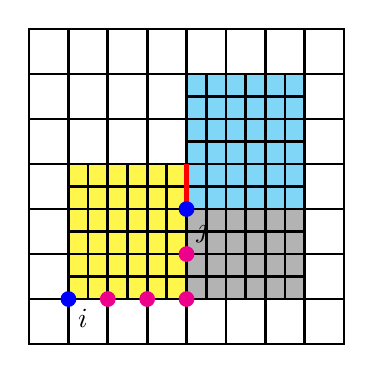
\begin{tikzpicture}[scale=4.0]
    % Define layers
    \pgfdeclarelayer{background}
    \pgfsetlayers{background,main}

    \coordinate (v1_1) at (0.0, 0.0);
    \coordinate (v1_2) at (0.125, 0.0);
    \coordinate (v1_3) at (0.125, 0.14285714285714285);
    \coordinate (v1_4) at (0.0, 0.14285714285714285);
    \draw[black, line width=1.0pt] (v1_1) -- (v1_2) -- (v1_3) -- (v1_4) -- cycle;
    \coordinate (v2_1) at (0.125, 0.0);
    \coordinate (v2_2) at (0.25, 0.0);
    \coordinate (v2_3) at (0.25, 0.14285714285714285);
    \coordinate (v2_4) at (0.125, 0.14285714285714285);
    \draw[black, line width=1.0pt] (v2_1) -- (v2_2) -- (v2_3) -- (v2_4) -- cycle;
    \coordinate (v3_1) at (0.25, 0.0);
    \coordinate (v3_2) at (0.375, 0.0);
    \coordinate (v3_3) at (0.375, 0.14285714285714285);
    \coordinate (v3_4) at (0.25, 0.14285714285714285);
    \draw[black, line width=1.0pt] (v3_1) -- (v3_2) -- (v3_3) -- (v3_4) -- cycle;
    \coordinate (v4_1) at (0.375, 0.0);
    \coordinate (v4_2) at (0.5, 0.0);
    \coordinate (v4_3) at (0.5, 0.14285714285714285);
    \coordinate (v4_4) at (0.375, 0.14285714285714285);
    \draw[black, line width=1.0pt] (v4_1) -- (v4_2) -- (v4_3) -- (v4_4) -- cycle;
    \coordinate (v5_1) at (0.5, 0.0);
    \coordinate (v5_2) at (0.625, 0.0);
    \coordinate (v5_3) at (0.625, 0.14285714285714285);
    \coordinate (v5_4) at (0.5, 0.14285714285714285);
    \draw[black, line width=1.0pt] (v5_1) -- (v5_2) -- (v5_3) -- (v5_4) -- cycle;
    \coordinate (v6_1) at (0.625, 0.0);
    \coordinate (v6_2) at (0.75, 0.0);
    \coordinate (v6_3) at (0.75, 0.14285714285714285);
    \coordinate (v6_4) at (0.625, 0.14285714285714285);
    \draw[black, line width=1.0pt] (v6_1) -- (v6_2) -- (v6_3) -- (v6_4) -- cycle;
    \coordinate (v7_1) at (0.75, 0.0);
    \coordinate (v7_2) at (0.875, 0.0);
    \coordinate (v7_3) at (0.875, 0.14285714285714285);
    \coordinate (v7_4) at (0.75, 0.14285714285714285);
    \draw[black, line width=1.0pt] (v7_1) -- (v7_2) -- (v7_3) -- (v7_4) -- cycle;
    \coordinate (v8_1) at (0.875, 0.0);
    \coordinate (v8_2) at (1.0, 0.0);
    \coordinate (v8_3) at (1.0, 0.14285714285714285);
    \coordinate (v8_4) at (0.875, 0.14285714285714285);
    \draw[black, line width=1.0pt] (v8_1) -- (v8_2) -- (v8_3) -- (v8_4) -- cycle;
    \coordinate (v9_1) at (0.0, 0.14285714285714285);
    \coordinate (v9_2) at (0.125, 0.14285714285714285);
    \coordinate (v9_3) at (0.125, 0.2857142857142857);
    \coordinate (v9_4) at (0.0, 0.2857142857142857);
    \draw[black, line width=1.0pt] (v9_1) -- (v9_2) -- (v9_3) -- (v9_4) -- cycle;
    \coordinate (v10_1) at (0.875, 0.14285714285714285);
    \coordinate (v10_2) at (1.0, 0.14285714285714285);
    \coordinate (v10_3) at (1.0, 0.2857142857142857);
    \coordinate (v10_4) at (0.875, 0.2857142857142857);
    \draw[black, line width=1.0pt] (v10_1) -- (v10_2) -- (v10_3) -- (v10_4) -- cycle;
    \coordinate (v11_1) at (0.0, 0.2857142857142857);
    \coordinate (v11_2) at (0.125, 0.2857142857142857);
    \coordinate (v11_3) at (0.125, 0.42857142857142855);
    \coordinate (v11_4) at (0.0, 0.42857142857142855);
    \draw[black, line width=1.0pt] (v11_1) -- (v11_2) -- (v11_3) -- (v11_4) -- cycle;
    \coordinate (v12_1) at (0.875, 0.2857142857142857);
    \coordinate (v12_2) at (1.0, 0.2857142857142857);
    \coordinate (v12_3) at (1.0, 0.42857142857142855);
    \coordinate (v12_4) at (0.875, 0.42857142857142855);
    \draw[black, line width=1.0pt] (v12_1) -- (v12_2) -- (v12_3) -- (v12_4) -- cycle;
    \coordinate (v13_1) at (0.0, 0.42857142857142855);
    \coordinate (v13_2) at (0.125, 0.42857142857142855);
    \coordinate (v13_3) at (0.125, 0.5714285714285714);
    \coordinate (v13_4) at (0.0, 0.5714285714285714);
    \draw[black, line width=1.0pt] (v13_1) -- (v13_2) -- (v13_3) -- (v13_4) -- cycle;
    \coordinate (v14_1) at (0.875, 0.42857142857142855);
    \coordinate (v14_2) at (1.0, 0.42857142857142855);
    \coordinate (v14_3) at (1.0, 0.5714285714285714);
    \coordinate (v14_4) at (0.875, 0.5714285714285714);
    \draw[black, line width=1.0pt] (v14_1) -- (v14_2) -- (v14_3) -- (v14_4) -- cycle;
    \coordinate (v15_1) at (0.0, 0.5714285714285714);
    \coordinate (v15_2) at (0.125, 0.5714285714285714);
    \coordinate (v15_3) at (0.125, 0.7142857142857143);
    \coordinate (v15_4) at (0.0, 0.7142857142857143);
    \draw[black, line width=1.0pt] (v15_1) -- (v15_2) -- (v15_3) -- (v15_4) -- cycle;
    \coordinate (v16_1) at (0.125, 0.5714285714285714);
    \coordinate (v16_2) at (0.25, 0.5714285714285714);
    \coordinate (v16_3) at (0.25, 0.7142857142857143);
    \coordinate (v16_4) at (0.125, 0.7142857142857143);
    \draw[black, line width=1.0pt] (v16_1) -- (v16_2) -- (v16_3) -- (v16_4) -- cycle;
    \coordinate (v17_1) at (0.25, 0.5714285714285714);
    \coordinate (v17_2) at (0.375, 0.5714285714285714);
    \coordinate (v17_3) at (0.375, 0.7142857142857143);
    \coordinate (v17_4) at (0.25, 0.7142857142857143);
    \draw[black, line width=1.0pt] (v17_1) -- (v17_2) -- (v17_3) -- (v17_4) -- cycle;
    \coordinate (v18_1) at (0.375, 0.5714285714285714);
    \coordinate (v18_2) at (0.5, 0.5714285714285714);
    \coordinate (v18_3) at (0.5, 0.7142857142857143);
    \coordinate (v18_4) at (0.375, 0.7142857142857143);
    \draw[black, line width=1.0pt] (v18_1) -- (v18_2) -- (v18_3) -- (v18_4) -- cycle;
    \coordinate (v19_1) at (0.875, 0.5714285714285714);
    \coordinate (v19_2) at (1.0, 0.5714285714285714);
    \coordinate (v19_3) at (1.0, 0.7142857142857143);
    \coordinate (v19_4) at (0.875, 0.7142857142857143);
    \draw[black, line width=1.0pt] (v19_1) -- (v19_2) -- (v19_3) -- (v19_4) -- cycle;
    \coordinate (v20_1) at (0.0, 0.7142857142857143);
    \coordinate (v20_2) at (0.125, 0.7142857142857143);
    \coordinate (v20_3) at (0.125, 0.8571428571428571);
    \coordinate (v20_4) at (0.0, 0.8571428571428571);
    \draw[black, line width=1.0pt] (v20_1) -- (v20_2) -- (v20_3) -- (v20_4) -- cycle;
    \coordinate (v21_1) at (0.125, 0.7142857142857143);
    \coordinate (v21_2) at (0.25, 0.7142857142857143);
    \coordinate (v21_3) at (0.25, 0.8571428571428571);
    \coordinate (v21_4) at (0.125, 0.8571428571428571);
    \draw[black, line width=1.0pt] (v21_1) -- (v21_2) -- (v21_3) -- (v21_4) -- cycle;
    \coordinate (v22_1) at (0.25, 0.7142857142857143);
    \coordinate (v22_2) at (0.375, 0.7142857142857143);
    \coordinate (v22_3) at (0.375, 0.8571428571428571);
    \coordinate (v22_4) at (0.25, 0.8571428571428571);
    \draw[black, line width=1.0pt] (v22_1) -- (v22_2) -- (v22_3) -- (v22_4) -- cycle;
    \coordinate (v23_1) at (0.375, 0.7142857142857143);
    \coordinate (v23_2) at (0.5, 0.7142857142857143);
    \coordinate (v23_3) at (0.5, 0.8571428571428571);
    \coordinate (v23_4) at (0.375, 0.8571428571428571);
    \draw[black, line width=1.0pt] (v23_1) -- (v23_2) -- (v23_3) -- (v23_4) -- cycle;
    \coordinate (v24_1) at (0.875, 0.7142857142857143);
    \coordinate (v24_2) at (1.0, 0.7142857142857143);
    \coordinate (v24_3) at (1.0, 0.8571428571428571);
    \coordinate (v24_4) at (0.875, 0.8571428571428571);
    \draw[black, line width=1.0pt] (v24_1) -- (v24_2) -- (v24_3) -- (v24_4) -- cycle;
    \coordinate (v25_1) at (0.0, 0.8571428571428571);
    \coordinate (v25_2) at (0.125, 0.8571428571428571);
    \coordinate (v25_3) at (0.125, 1.0);
    \coordinate (v25_4) at (0.0, 1.0);
    \draw[black, line width=1.0pt] (v25_1) -- (v25_2) -- (v25_3) -- (v25_4) -- cycle;
    \coordinate (v26_1) at (0.125, 0.8571428571428571);
    \coordinate (v26_2) at (0.25, 0.8571428571428571);
    \coordinate (v26_3) at (0.25, 1.0);
    \coordinate (v26_4) at (0.125, 1.0);
    \draw[black, line width=1.0pt] (v26_1) -- (v26_2) -- (v26_3) -- (v26_4) -- cycle;
    \coordinate (v27_1) at (0.25, 0.8571428571428571);
    \coordinate (v27_2) at (0.375, 0.8571428571428571);
    \coordinate (v27_3) at (0.375, 1.0);
    \coordinate (v27_4) at (0.25, 1.0);
    \draw[black, line width=1.0pt] (v27_1) -- (v27_2) -- (v27_3) -- (v27_4) -- cycle;
    \coordinate (v28_1) at (0.375, 0.8571428571428571);
    \coordinate (v28_2) at (0.5, 0.8571428571428571);
    \coordinate (v28_3) at (0.5, 1.0);
    \coordinate (v28_4) at (0.375, 1.0);
    \draw[black, line width=1.0pt] (v28_1) -- (v28_2) -- (v28_3) -- (v28_4) -- cycle;
    \coordinate (v29_1) at (0.5, 0.8571428571428571);
    \coordinate (v29_2) at (0.625, 0.8571428571428571);
    \coordinate (v29_3) at (0.625, 1.0);
    \coordinate (v29_4) at (0.5, 1.0);
    \draw[black, line width=1.0pt] (v29_1) -- (v29_2) -- (v29_3) -- (v29_4) -- cycle;
    \coordinate (v30_1) at (0.625, 0.8571428571428571);
    \coordinate (v30_2) at (0.75, 0.8571428571428571);
    \coordinate (v30_3) at (0.75, 1.0);
    \coordinate (v30_4) at (0.625, 1.0);
    \draw[black, line width=1.0pt] (v30_1) -- (v30_2) -- (v30_3) -- (v30_4) -- cycle;
    \coordinate (v31_1) at (0.75, 0.8571428571428571);
    \coordinate (v31_2) at (0.875, 0.8571428571428571);
    \coordinate (v31_3) at (0.875, 1.0);
    \coordinate (v31_4) at (0.75, 1.0);
    \draw[black, line width=1.0pt] (v31_1) -- (v31_2) -- (v31_3) -- (v31_4) -- cycle;
    \coordinate (v32_1) at (0.875, 0.8571428571428571);
    \coordinate (v32_2) at (1.0, 0.8571428571428571);
    \coordinate (v32_3) at (1.0, 1.0);
    \coordinate (v32_4) at (0.875, 1.0);
    \draw[black, line width=1.0pt] (v32_1) -- (v32_2) -- (v32_3) -- (v32_4) -- cycle;
    \coordinate (v33_1) at (0.125, 0.14285714285714285);
    \coordinate (v33_2) at (0.1875, 0.14285714285714285);
    \coordinate (v33_3) at (0.1875, 0.21428571428571427);
    \coordinate (v33_4) at (0.125, 0.21428571428571427);
    \draw[black, line width=1.0pt] (v33_1) -- (v33_2) -- (v33_3) -- (v33_4) -- cycle;
    \coordinate (v34_1) at (0.1875, 0.14285714285714285);
    \coordinate (v34_2) at (0.25, 0.14285714285714285);
    \coordinate (v34_3) at (0.25, 0.21428571428571427);
    \coordinate (v34_4) at (0.1875, 0.21428571428571427);
    \draw[black, line width=1.0pt] (v34_1) -- (v34_2) -- (v34_3) -- (v34_4) -- cycle;
    \coordinate (v35_1) at (0.25, 0.14285714285714285);
    \coordinate (v35_2) at (0.3125, 0.14285714285714285);
    \coordinate (v35_3) at (0.3125, 0.21428571428571427);
    \coordinate (v35_4) at (0.25, 0.21428571428571427);
    \draw[black, line width=1.0pt] (v35_1) -- (v35_2) -- (v35_3) -- (v35_4) -- cycle;
    \coordinate (v36_1) at (0.3125, 0.14285714285714285);
    \coordinate (v36_2) at (0.375, 0.14285714285714285);
    \coordinate (v36_3) at (0.375, 0.21428571428571427);
    \coordinate (v36_4) at (0.3125, 0.21428571428571427);
    \draw[black, line width=1.0pt] (v36_1) -- (v36_2) -- (v36_3) -- (v36_4) -- cycle;
    \coordinate (v37_1) at (0.375, 0.14285714285714285);
    \coordinate (v37_2) at (0.4375, 0.14285714285714285);
    \coordinate (v37_3) at (0.4375, 0.21428571428571427);
    \coordinate (v37_4) at (0.375, 0.21428571428571427);
    \draw[black, line width=1.0pt] (v37_1) -- (v37_2) -- (v37_3) -- (v37_4) -- cycle;
    \coordinate (v38_1) at (0.4375, 0.14285714285714285);
    \coordinate (v38_2) at (0.5, 0.14285714285714285);
    \coordinate (v38_3) at (0.5, 0.21428571428571427);
    \coordinate (v38_4) at (0.4375, 0.21428571428571427);
    \draw[black, line width=1.0pt] (v38_1) -- (v38_2) -- (v38_3) -- (v38_4) -- cycle;
    \coordinate (v39_1) at (0.5, 0.14285714285714285);
    \coordinate (v39_2) at (0.5625, 0.14285714285714285);
    \coordinate (v39_3) at (0.5625, 0.21428571428571427);
    \coordinate (v39_4) at (0.5, 0.21428571428571427);
    \draw[black, line width=1.0pt] (v39_1) -- (v39_2) -- (v39_3) -- (v39_4) -- cycle;
    \coordinate (v40_1) at (0.5625, 0.14285714285714285);
    \coordinate (v40_2) at (0.625, 0.14285714285714285);
    \coordinate (v40_3) at (0.625, 0.21428571428571427);
    \coordinate (v40_4) at (0.5625, 0.21428571428571427);
    \draw[black, line width=1.0pt] (v40_1) -- (v40_2) -- (v40_3) -- (v40_4) -- cycle;
    \coordinate (v41_1) at (0.625, 0.14285714285714285);
    \coordinate (v41_2) at (0.6875, 0.14285714285714285);
    \coordinate (v41_3) at (0.6875, 0.21428571428571427);
    \coordinate (v41_4) at (0.625, 0.21428571428571427);
    \draw[black, line width=1.0pt] (v41_1) -- (v41_2) -- (v41_3) -- (v41_4) -- cycle;
    \coordinate (v42_1) at (0.6875, 0.14285714285714285);
    \coordinate (v42_2) at (0.75, 0.14285714285714285);
    \coordinate (v42_3) at (0.75, 0.21428571428571427);
    \coordinate (v42_4) at (0.6875, 0.21428571428571427);
    \draw[black, line width=1.0pt] (v42_1) -- (v42_2) -- (v42_3) -- (v42_4) -- cycle;
    \coordinate (v43_1) at (0.75, 0.14285714285714285);
    \coordinate (v43_2) at (0.8125, 0.14285714285714285);
    \coordinate (v43_3) at (0.8125, 0.21428571428571427);
    \coordinate (v43_4) at (0.75, 0.21428571428571427);
    \draw[black, line width=1.0pt] (v43_1) -- (v43_2) -- (v43_3) -- (v43_4) -- cycle;
    \coordinate (v44_1) at (0.8125, 0.14285714285714285);
    \coordinate (v44_2) at (0.875, 0.14285714285714285);
    \coordinate (v44_3) at (0.875, 0.21428571428571427);
    \coordinate (v44_4) at (0.8125, 0.21428571428571427);
    \draw[black, line width=1.0pt] (v44_1) -- (v44_2) -- (v44_3) -- (v44_4) -- cycle;
    \coordinate (v45_1) at (0.125, 0.21428571428571427);
    \coordinate (v45_2) at (0.1875, 0.21428571428571427);
    \coordinate (v45_3) at (0.1875, 0.2857142857142857);
    \coordinate (v45_4) at (0.125, 0.2857142857142857);
    \draw[black, line width=1.0pt] (v45_1) -- (v45_2) -- (v45_3) -- (v45_4) -- cycle;
    \coordinate (v46_1) at (0.1875, 0.21428571428571427);
    \coordinate (v46_2) at (0.25, 0.21428571428571427);
    \coordinate (v46_3) at (0.25, 0.2857142857142857);
    \coordinate (v46_4) at (0.1875, 0.2857142857142857);
    \draw[black, line width=1.0pt] (v46_1) -- (v46_2) -- (v46_3) -- (v46_4) -- cycle;
    \coordinate (v47_1) at (0.25, 0.21428571428571427);
    \coordinate (v47_2) at (0.3125, 0.21428571428571427);
    \coordinate (v47_3) at (0.3125, 0.2857142857142857);
    \coordinate (v47_4) at (0.25, 0.2857142857142857);
    \draw[black, line width=1.0pt] (v47_1) -- (v47_2) -- (v47_3) -- (v47_4) -- cycle;
    \coordinate (v48_1) at (0.3125, 0.21428571428571427);
    \coordinate (v48_2) at (0.375, 0.21428571428571427);
    \coordinate (v48_3) at (0.375, 0.2857142857142857);
    \coordinate (v48_4) at (0.3125, 0.2857142857142857);
    \draw[black, line width=1.0pt] (v48_1) -- (v48_2) -- (v48_3) -- (v48_4) -- cycle;
    \coordinate (v49_1) at (0.375, 0.21428571428571427);
    \coordinate (v49_2) at (0.4375, 0.21428571428571427);
    \coordinate (v49_3) at (0.4375, 0.2857142857142857);
    \coordinate (v49_4) at (0.375, 0.2857142857142857);
    \draw[black, line width=1.0pt] (v49_1) -- (v49_2) -- (v49_3) -- (v49_4) -- cycle;
    \coordinate (v50_1) at (0.4375, 0.21428571428571427);
    \coordinate (v50_2) at (0.5, 0.21428571428571427);
    \coordinate (v50_3) at (0.5, 0.2857142857142857);
    \coordinate (v50_4) at (0.4375, 0.2857142857142857);
    \draw[black, line width=1.0pt] (v50_1) -- (v50_2) -- (v50_3) -- (v50_4) -- cycle;
    \coordinate (v51_1) at (0.5, 0.21428571428571427);
    \coordinate (v51_2) at (0.5625, 0.21428571428571427);
    \coordinate (v51_3) at (0.5625, 0.2857142857142857);
    \coordinate (v51_4) at (0.5, 0.2857142857142857);
    \draw[black, line width=1.0pt] (v51_1) -- (v51_2) -- (v51_3) -- (v51_4) -- cycle;
    \coordinate (v52_1) at (0.5625, 0.21428571428571427);
    \coordinate (v52_2) at (0.625, 0.21428571428571427);
    \coordinate (v52_3) at (0.625, 0.2857142857142857);
    \coordinate (v52_4) at (0.5625, 0.2857142857142857);
    \draw[black, line width=1.0pt] (v52_1) -- (v52_2) -- (v52_3) -- (v52_4) -- cycle;
    \coordinate (v53_1) at (0.625, 0.21428571428571427);
    \coordinate (v53_2) at (0.6875, 0.21428571428571427);
    \coordinate (v53_3) at (0.6875, 0.2857142857142857);
    \coordinate (v53_4) at (0.625, 0.2857142857142857);
    \draw[black, line width=1.0pt] (v53_1) -- (v53_2) -- (v53_3) -- (v53_4) -- cycle;
    \coordinate (v54_1) at (0.6875, 0.21428571428571427);
    \coordinate (v54_2) at (0.75, 0.21428571428571427);
    \coordinate (v54_3) at (0.75, 0.2857142857142857);
    \coordinate (v54_4) at (0.6875, 0.2857142857142857);
    \draw[black, line width=1.0pt] (v54_1) -- (v54_2) -- (v54_3) -- (v54_4) -- cycle;
    \coordinate (v55_1) at (0.75, 0.21428571428571427);
    \coordinate (v55_2) at (0.8125, 0.21428571428571427);
    \coordinate (v55_3) at (0.8125, 0.2857142857142857);
    \coordinate (v55_4) at (0.75, 0.2857142857142857);
    \draw[black, line width=1.0pt] (v55_1) -- (v55_2) -- (v55_3) -- (v55_4) -- cycle;
    \coordinate (v56_1) at (0.8125, 0.21428571428571427);
    \coordinate (v56_2) at (0.875, 0.21428571428571427);
    \coordinate (v56_3) at (0.875, 0.2857142857142857);
    \coordinate (v56_4) at (0.8125, 0.2857142857142857);
    \draw[black, line width=1.0pt] (v56_1) -- (v56_2) -- (v56_3) -- (v56_4) -- cycle;
    \coordinate (v57_1) at (0.125, 0.2857142857142857);
    \coordinate (v57_2) at (0.1875, 0.2857142857142857);
    \coordinate (v57_3) at (0.1875, 0.3571428571428571);
    \coordinate (v57_4) at (0.125, 0.3571428571428571);
    \draw[black, line width=1.0pt] (v57_1) -- (v57_2) -- (v57_3) -- (v57_4) -- cycle;
    \coordinate (v58_1) at (0.1875, 0.2857142857142857);
    \coordinate (v58_2) at (0.25, 0.2857142857142857);
    \coordinate (v58_3) at (0.25, 0.3571428571428571);
    \coordinate (v58_4) at (0.1875, 0.3571428571428571);
    \draw[black, line width=1.0pt] (v58_1) -- (v58_2) -- (v58_3) -- (v58_4) -- cycle;
    \coordinate (v59_1) at (0.25, 0.2857142857142857);
    \coordinate (v59_2) at (0.3125, 0.2857142857142857);
    \coordinate (v59_3) at (0.3125, 0.3571428571428571);
    \coordinate (v59_4) at (0.25, 0.3571428571428571);
    \draw[black, line width=1.0pt] (v59_1) -- (v59_2) -- (v59_3) -- (v59_4) -- cycle;
    \coordinate (v60_1) at (0.3125, 0.2857142857142857);
    \coordinate (v60_2) at (0.375, 0.2857142857142857);
    \coordinate (v60_3) at (0.375, 0.3571428571428571);
    \coordinate (v60_4) at (0.3125, 0.3571428571428571);
    \draw[black, line width=1.0pt] (v60_1) -- (v60_2) -- (v60_3) -- (v60_4) -- cycle;
    \coordinate (v61_1) at (0.375, 0.2857142857142857);
    \coordinate (v61_2) at (0.4375, 0.2857142857142857);
    \coordinate (v61_3) at (0.4375, 0.3571428571428571);
    \coordinate (v61_4) at (0.375, 0.3571428571428571);
    \draw[black, line width=1.0pt] (v61_1) -- (v61_2) -- (v61_3) -- (v61_4) -- cycle;
    \coordinate (v62_1) at (0.4375, 0.2857142857142857);
    \coordinate (v62_2) at (0.5, 0.2857142857142857);
    \coordinate (v62_3) at (0.5, 0.3571428571428571);
    \coordinate (v62_4) at (0.4375, 0.3571428571428571);
    \draw[black, line width=1.0pt] (v62_1) -- (v62_2) -- (v62_3) -- (v62_4) -- cycle;
    \coordinate (v63_1) at (0.5, 0.2857142857142857);
    \coordinate (v63_2) at (0.5625, 0.2857142857142857);
    \coordinate (v63_3) at (0.5625, 0.3571428571428571);
    \coordinate (v63_4) at (0.5, 0.3571428571428571);
    \draw[black, line width=1.0pt] (v63_1) -- (v63_2) -- (v63_3) -- (v63_4) -- cycle;
    \coordinate (v64_1) at (0.5625, 0.2857142857142857);
    \coordinate (v64_2) at (0.625, 0.2857142857142857);
    \coordinate (v64_3) at (0.625, 0.3571428571428571);
    \coordinate (v64_4) at (0.5625, 0.3571428571428571);
    \draw[black, line width=1.0pt] (v64_1) -- (v64_2) -- (v64_3) -- (v64_4) -- cycle;
    \coordinate (v65_1) at (0.625, 0.2857142857142857);
    \coordinate (v65_2) at (0.6875, 0.2857142857142857);
    \coordinate (v65_3) at (0.6875, 0.3571428571428571);
    \coordinate (v65_4) at (0.625, 0.3571428571428571);
    \draw[black, line width=1.0pt] (v65_1) -- (v65_2) -- (v65_3) -- (v65_4) -- cycle;
    \coordinate (v66_1) at (0.6875, 0.2857142857142857);
    \coordinate (v66_2) at (0.75, 0.2857142857142857);
    \coordinate (v66_3) at (0.75, 0.3571428571428571);
    \coordinate (v66_4) at (0.6875, 0.3571428571428571);
    \draw[black, line width=1.0pt] (v66_1) -- (v66_2) -- (v66_3) -- (v66_4) -- cycle;
    \coordinate (v67_1) at (0.75, 0.2857142857142857);
    \coordinate (v67_2) at (0.8125, 0.2857142857142857);
    \coordinate (v67_3) at (0.8125, 0.3571428571428571);
    \coordinate (v67_4) at (0.75, 0.3571428571428571);
    \draw[black, line width=1.0pt] (v67_1) -- (v67_2) -- (v67_3) -- (v67_4) -- cycle;
    \coordinate (v68_1) at (0.8125, 0.2857142857142857);
    \coordinate (v68_2) at (0.875, 0.2857142857142857);
    \coordinate (v68_3) at (0.875, 0.3571428571428571);
    \coordinate (v68_4) at (0.8125, 0.3571428571428571);
    \draw[black, line width=1.0pt] (v68_1) -- (v68_2) -- (v68_3) -- (v68_4) -- cycle;
    \coordinate (v69_1) at (0.125, 0.3571428571428571);
    \coordinate (v69_2) at (0.1875, 0.3571428571428571);
    \coordinate (v69_3) at (0.1875, 0.42857142857142855);
    \coordinate (v69_4) at (0.125, 0.42857142857142855);
    \draw[black, line width=1.0pt] (v69_1) -- (v69_2) -- (v69_3) -- (v69_4) -- cycle;
    \coordinate (v70_1) at (0.1875, 0.3571428571428571);
    \coordinate (v70_2) at (0.25, 0.3571428571428571);
    \coordinate (v70_3) at (0.25, 0.42857142857142855);
    \coordinate (v70_4) at (0.1875, 0.42857142857142855);
    \draw[black, line width=1.0pt] (v70_1) -- (v70_2) -- (v70_3) -- (v70_4) -- cycle;
    \coordinate (v71_1) at (0.25, 0.3571428571428571);
    \coordinate (v71_2) at (0.3125, 0.3571428571428571);
    \coordinate (v71_3) at (0.3125, 0.42857142857142855);
    \coordinate (v71_4) at (0.25, 0.42857142857142855);
    \draw[black, line width=1.0pt] (v71_1) -- (v71_2) -- (v71_3) -- (v71_4) -- cycle;
    \coordinate (v72_1) at (0.3125, 0.3571428571428571);
    \coordinate (v72_2) at (0.375, 0.3571428571428571);
    \coordinate (v72_3) at (0.375, 0.42857142857142855);
    \coordinate (v72_4) at (0.3125, 0.42857142857142855);
    \draw[black, line width=1.0pt] (v72_1) -- (v72_2) -- (v72_3) -- (v72_4) -- cycle;
    \coordinate (v73_1) at (0.375, 0.3571428571428571);
    \coordinate (v73_2) at (0.4375, 0.3571428571428571);
    \coordinate (v73_3) at (0.4375, 0.42857142857142855);
    \coordinate (v73_4) at (0.375, 0.42857142857142855);
    \draw[black, line width=1.0pt] (v73_1) -- (v73_2) -- (v73_3) -- (v73_4) -- cycle;
    \coordinate (v74_1) at (0.4375, 0.3571428571428571);
    \coordinate (v74_2) at (0.5, 0.3571428571428571);
    \coordinate (v74_3) at (0.5, 0.42857142857142855);
    \coordinate (v74_4) at (0.4375, 0.42857142857142855);
    \draw[black, line width=1.0pt] (v74_1) -- (v74_2) -- (v74_3) -- (v74_4) -- cycle;
    \coordinate (v75_1) at (0.5, 0.3571428571428571);
    \coordinate (v75_2) at (0.5625, 0.3571428571428571);
    \coordinate (v75_3) at (0.5625, 0.42857142857142855);
    \coordinate (v75_4) at (0.5, 0.42857142857142855);
    \draw[black, line width=1.0pt] (v75_1) -- (v75_2) -- (v75_3) -- (v75_4) -- cycle;
    \coordinate (v76_1) at (0.5625, 0.3571428571428571);
    \coordinate (v76_2) at (0.625, 0.3571428571428571);
    \coordinate (v76_3) at (0.625, 0.42857142857142855);
    \coordinate (v76_4) at (0.5625, 0.42857142857142855);
    \draw[black, line width=1.0pt] (v76_1) -- (v76_2) -- (v76_3) -- (v76_4) -- cycle;
    \coordinate (v77_1) at (0.625, 0.3571428571428571);
    \coordinate (v77_2) at (0.6875, 0.3571428571428571);
    \coordinate (v77_3) at (0.6875, 0.42857142857142855);
    \coordinate (v77_4) at (0.625, 0.42857142857142855);
    \draw[black, line width=1.0pt] (v77_1) -- (v77_2) -- (v77_3) -- (v77_4) -- cycle;
    \coordinate (v78_1) at (0.6875, 0.3571428571428571);
    \coordinate (v78_2) at (0.75, 0.3571428571428571);
    \coordinate (v78_3) at (0.75, 0.42857142857142855);
    \coordinate (v78_4) at (0.6875, 0.42857142857142855);
    \draw[black, line width=1.0pt] (v78_1) -- (v78_2) -- (v78_3) -- (v78_4) -- cycle;
    \coordinate (v79_1) at (0.75, 0.3571428571428571);
    \coordinate (v79_2) at (0.8125, 0.3571428571428571);
    \coordinate (v79_3) at (0.8125, 0.42857142857142855);
    \coordinate (v79_4) at (0.75, 0.42857142857142855);
    \draw[black, line width=1.0pt] (v79_1) -- (v79_2) -- (v79_3) -- (v79_4) -- cycle;
    \coordinate (v80_1) at (0.8125, 0.3571428571428571);
    \coordinate (v80_2) at (0.875, 0.3571428571428571);
    \coordinate (v80_3) at (0.875, 0.42857142857142855);
    \coordinate (v80_4) at (0.8125, 0.42857142857142855);
    \draw[black, line width=1.0pt] (v80_1) -- (v80_2) -- (v80_3) -- (v80_4) -- cycle;
    \coordinate (v81_1) at (0.125, 0.42857142857142855);
    \coordinate (v81_2) at (0.1875, 0.42857142857142855);
    \coordinate (v81_3) at (0.1875, 0.5);
    \coordinate (v81_4) at (0.125, 0.5);
    \draw[black, line width=1.0pt] (v81_1) -- (v81_2) -- (v81_3) -- (v81_4) -- cycle;
    \coordinate (v82_1) at (0.1875, 0.42857142857142855);
    \coordinate (v82_2) at (0.25, 0.42857142857142855);
    \coordinate (v82_3) at (0.25, 0.5);
    \coordinate (v82_4) at (0.1875, 0.5);
    \draw[black, line width=1.0pt] (v82_1) -- (v82_2) -- (v82_3) -- (v82_4) -- cycle;
    \coordinate (v83_1) at (0.25, 0.42857142857142855);
    \coordinate (v83_2) at (0.3125, 0.42857142857142855);
    \coordinate (v83_3) at (0.3125, 0.5);
    \coordinate (v83_4) at (0.25, 0.5);
    \draw[black, line width=1.0pt] (v83_1) -- (v83_2) -- (v83_3) -- (v83_4) -- cycle;
    \coordinate (v84_1) at (0.3125, 0.42857142857142855);
    \coordinate (v84_2) at (0.375, 0.42857142857142855);
    \coordinate (v84_3) at (0.375, 0.5);
    \coordinate (v84_4) at (0.3125, 0.5);
    \draw[black, line width=1.0pt] (v84_1) -- (v84_2) -- (v84_3) -- (v84_4) -- cycle;
    \coordinate (v85_1) at (0.375, 0.42857142857142855);
    \coordinate (v85_2) at (0.4375, 0.42857142857142855);
    \coordinate (v85_3) at (0.4375, 0.5);
    \coordinate (v85_4) at (0.375, 0.5);
    \draw[black, line width=1.0pt] (v85_1) -- (v85_2) -- (v85_3) -- (v85_4) -- cycle;
    \coordinate (v86_1) at (0.4375, 0.42857142857142855);
    \coordinate (v86_2) at (0.5, 0.42857142857142855);
    \coordinate (v86_3) at (0.5, 0.5);
    \coordinate (v86_4) at (0.4375, 0.5);
    \draw[black, line width=1.0pt] (v86_1) -- (v86_2) -- (v86_3) -- (v86_4) -- cycle;
    \coordinate (v87_1) at (0.5, 0.42857142857142855);
    \coordinate (v87_2) at (0.5625, 0.42857142857142855);
    \coordinate (v87_3) at (0.5625, 0.5);
    \coordinate (v87_4) at (0.5, 0.5);
    \draw[black, line width=1.0pt] (v87_1) -- (v87_2) -- (v87_3) -- (v87_4) -- cycle;
    \coordinate (v88_1) at (0.5625, 0.42857142857142855);
    \coordinate (v88_2) at (0.625, 0.42857142857142855);
    \coordinate (v88_3) at (0.625, 0.5);
    \coordinate (v88_4) at (0.5625, 0.5);
    \draw[black, line width=1.0pt] (v88_1) -- (v88_2) -- (v88_3) -- (v88_4) -- cycle;
    \coordinate (v89_1) at (0.625, 0.42857142857142855);
    \coordinate (v89_2) at (0.6875, 0.42857142857142855);
    \coordinate (v89_3) at (0.6875, 0.5);
    \coordinate (v89_4) at (0.625, 0.5);
    \draw[black, line width=1.0pt] (v89_1) -- (v89_2) -- (v89_3) -- (v89_4) -- cycle;
    \coordinate (v90_1) at (0.6875, 0.42857142857142855);
    \coordinate (v90_2) at (0.75, 0.42857142857142855);
    \coordinate (v90_3) at (0.75, 0.5);
    \coordinate (v90_4) at (0.6875, 0.5);
    \draw[black, line width=1.0pt] (v90_1) -- (v90_2) -- (v90_3) -- (v90_4) -- cycle;
    \coordinate (v91_1) at (0.75, 0.42857142857142855);
    \coordinate (v91_2) at (0.8125, 0.42857142857142855);
    \coordinate (v91_3) at (0.8125, 0.5);
    \coordinate (v91_4) at (0.75, 0.5);
    \draw[black, line width=1.0pt] (v91_1) -- (v91_2) -- (v91_3) -- (v91_4) -- cycle;
    \coordinate (v92_1) at (0.8125, 0.42857142857142855);
    \coordinate (v92_2) at (0.875, 0.42857142857142855);
    \coordinate (v92_3) at (0.875, 0.5);
    \coordinate (v92_4) at (0.8125, 0.5);
    \draw[black, line width=1.0pt] (v92_1) -- (v92_2) -- (v92_3) -- (v92_4) -- cycle;
    \coordinate (v93_1) at (0.125, 0.5);
    \coordinate (v93_2) at (0.1875, 0.5);
    \coordinate (v93_3) at (0.1875, 0.5714285714285714);
    \coordinate (v93_4) at (0.125, 0.5714285714285714);
    \draw[black, line width=1.0pt] (v93_1) -- (v93_2) -- (v93_3) -- (v93_4) -- cycle;
    \coordinate (v94_1) at (0.1875, 0.5);
    \coordinate (v94_2) at (0.25, 0.5);
    \coordinate (v94_3) at (0.25, 0.5714285714285714);
    \coordinate (v94_4) at (0.1875, 0.5714285714285714);
    \draw[black, line width=1.0pt] (v94_1) -- (v94_2) -- (v94_3) -- (v94_4) -- cycle;
    \coordinate (v95_1) at (0.25, 0.5);
    \coordinate (v95_2) at (0.3125, 0.5);
    \coordinate (v95_3) at (0.3125, 0.5714285714285714);
    \coordinate (v95_4) at (0.25, 0.5714285714285714);
    \draw[black, line width=1.0pt] (v95_1) -- (v95_2) -- (v95_3) -- (v95_4) -- cycle;
    \coordinate (v96_1) at (0.3125, 0.5);
    \coordinate (v96_2) at (0.375, 0.5);
    \coordinate (v96_3) at (0.375, 0.5714285714285714);
    \coordinate (v96_4) at (0.3125, 0.5714285714285714);
    \draw[black, line width=1.0pt] (v96_1) -- (v96_2) -- (v96_3) -- (v96_4) -- cycle;
    \coordinate (v97_1) at (0.375, 0.5);
    \coordinate (v97_2) at (0.4375, 0.5);
    \coordinate (v97_3) at (0.4375, 0.5714285714285714);
    \coordinate (v97_4) at (0.375, 0.5714285714285714);
    \draw[black, line width=1.0pt] (v97_1) -- (v97_2) -- (v97_3) -- (v97_4) -- cycle;
    \coordinate (v98_1) at (0.4375, 0.5);
    \coordinate (v98_2) at (0.5, 0.5);
    \coordinate (v98_3) at (0.5, 0.5714285714285714);
    \coordinate (v98_4) at (0.4375, 0.5714285714285714);
    \draw[black, line width=1.0pt] (v98_1) -- (v98_2) -- (v98_3) -- (v98_4) -- cycle;
    \coordinate (v99_1) at (0.5, 0.5);
    \coordinate (v99_2) at (0.5625, 0.5);
    \coordinate (v99_3) at (0.5625, 0.5714285714285714);
    \coordinate (v99_4) at (0.5, 0.5714285714285714);
    \draw[black, line width=1.0pt] (v99_1) -- (v99_2) -- (v99_3) -- (v99_4) -- cycle;
    \coordinate (v100_1) at (0.5625, 0.5);
    \coordinate (v100_2) at (0.625, 0.5);
    \coordinate (v100_3) at (0.625, 0.5714285714285714);
    \coordinate (v100_4) at (0.5625, 0.5714285714285714);
    \draw[black, line width=1.0pt] (v100_1) -- (v100_2) -- (v100_3) -- (v100_4) -- cycle;
    \coordinate (v101_1) at (0.625, 0.5);
    \coordinate (v101_2) at (0.6875, 0.5);
    \coordinate (v101_3) at (0.6875, 0.5714285714285714);
    \coordinate (v101_4) at (0.625, 0.5714285714285714);
    \draw[black, line width=1.0pt] (v101_1) -- (v101_2) -- (v101_3) -- (v101_4) -- cycle;
    \coordinate (v102_1) at (0.6875, 0.5);
    \coordinate (v102_2) at (0.75, 0.5);
    \coordinate (v102_3) at (0.75, 0.5714285714285714);
    \coordinate (v102_4) at (0.6875, 0.5714285714285714);
    \draw[black, line width=1.0pt] (v102_1) -- (v102_2) -- (v102_3) -- (v102_4) -- cycle;
    \coordinate (v103_1) at (0.75, 0.5);
    \coordinate (v103_2) at (0.8125, 0.5);
    \coordinate (v103_3) at (0.8125, 0.5714285714285714);
    \coordinate (v103_4) at (0.75, 0.5714285714285714);
    \draw[black, line width=1.0pt] (v103_1) -- (v103_2) -- (v103_3) -- (v103_4) -- cycle;
    \coordinate (v104_1) at (0.8125, 0.5);
    \coordinate (v104_2) at (0.875, 0.5);
    \coordinate (v104_3) at (0.875, 0.5714285714285714);
    \coordinate (v104_4) at (0.8125, 0.5714285714285714);
    \draw[black, line width=1.0pt] (v104_1) -- (v104_2) -- (v104_3) -- (v104_4) -- cycle;
    \coordinate (v105_1) at (0.5, 0.5714285714285714);
    \coordinate (v105_2) at (0.5625, 0.5714285714285714);
    \coordinate (v105_3) at (0.5625, 0.6428571428571428);
    \coordinate (v105_4) at (0.5, 0.6428571428571428);
    \draw[black, line width=1.0pt] (v105_1) -- (v105_2) -- (v105_3) -- (v105_4) -- cycle;
    \coordinate (v106_1) at (0.5625, 0.5714285714285714);
    \coordinate (v106_2) at (0.625, 0.5714285714285714);
    \coordinate (v106_3) at (0.625, 0.6428571428571428);
    \coordinate (v106_4) at (0.5625, 0.6428571428571428);
    \draw[black, line width=1.0pt] (v106_1) -- (v106_2) -- (v106_3) -- (v106_4) -- cycle;
    \coordinate (v107_1) at (0.625, 0.5714285714285714);
    \coordinate (v107_2) at (0.6875, 0.5714285714285714);
    \coordinate (v107_3) at (0.6875, 0.6428571428571428);
    \coordinate (v107_4) at (0.625, 0.6428571428571428);
    \draw[black, line width=1.0pt] (v107_1) -- (v107_2) -- (v107_3) -- (v107_4) -- cycle;
    \coordinate (v108_1) at (0.6875, 0.5714285714285714);
    \coordinate (v108_2) at (0.75, 0.5714285714285714);
    \coordinate (v108_3) at (0.75, 0.6428571428571428);
    \coordinate (v108_4) at (0.6875, 0.6428571428571428);
    \draw[black, line width=1.0pt] (v108_1) -- (v108_2) -- (v108_3) -- (v108_4) -- cycle;
    \coordinate (v109_1) at (0.75, 0.5714285714285714);
    \coordinate (v109_2) at (0.8125, 0.5714285714285714);
    \coordinate (v109_3) at (0.8125, 0.6428571428571428);
    \coordinate (v109_4) at (0.75, 0.6428571428571428);
    \draw[black, line width=1.0pt] (v109_1) -- (v109_2) -- (v109_3) -- (v109_4) -- cycle;
    \coordinate (v110_1) at (0.8125, 0.5714285714285714);
    \coordinate (v110_2) at (0.875, 0.5714285714285714);
    \coordinate (v110_3) at (0.875, 0.6428571428571428);
    \coordinate (v110_4) at (0.8125, 0.6428571428571428);
    \draw[black, line width=1.0pt] (v110_1) -- (v110_2) -- (v110_3) -- (v110_4) -- cycle;
    \coordinate (v111_1) at (0.5, 0.6428571428571428);
    \coordinate (v111_2) at (0.5625, 0.6428571428571428);
    \coordinate (v111_3) at (0.5625, 0.7142857142857143);
    \coordinate (v111_4) at (0.5, 0.7142857142857143);
    \draw[black, line width=1.0pt] (v111_1) -- (v111_2) -- (v111_3) -- (v111_4) -- cycle;
    \coordinate (v112_1) at (0.5625, 0.6428571428571428);
    \coordinate (v112_2) at (0.625, 0.6428571428571428);
    \coordinate (v112_3) at (0.625, 0.7142857142857143);
    \coordinate (v112_4) at (0.5625, 0.7142857142857143);
    \draw[black, line width=1.0pt] (v112_1) -- (v112_2) -- (v112_3) -- (v112_4) -- cycle;
    \coordinate (v113_1) at (0.625, 0.6428571428571428);
    \coordinate (v113_2) at (0.6875, 0.6428571428571428);
    \coordinate (v113_3) at (0.6875, 0.7142857142857143);
    \coordinate (v113_4) at (0.625, 0.7142857142857143);
    \draw[black, line width=1.0pt] (v113_1) -- (v113_2) -- (v113_3) -- (v113_4) -- cycle;
    \coordinate (v114_1) at (0.6875, 0.6428571428571428);
    \coordinate (v114_2) at (0.75, 0.6428571428571428);
    \coordinate (v114_3) at (0.75, 0.7142857142857143);
    \coordinate (v114_4) at (0.6875, 0.7142857142857143);
    \draw[black, line width=1.0pt] (v114_1) -- (v114_2) -- (v114_3) -- (v114_4) -- cycle;
    \coordinate (v115_1) at (0.75, 0.6428571428571428);
    \coordinate (v115_2) at (0.8125, 0.6428571428571428);
    \coordinate (v115_3) at (0.8125, 0.7142857142857143);
    \coordinate (v115_4) at (0.75, 0.7142857142857143);
    \draw[black, line width=1.0pt] (v115_1) -- (v115_2) -- (v115_3) -- (v115_4) -- cycle;
    \coordinate (v116_1) at (0.8125, 0.6428571428571428);
    \coordinate (v116_2) at (0.875, 0.6428571428571428);
    \coordinate (v116_3) at (0.875, 0.7142857142857143);
    \coordinate (v116_4) at (0.8125, 0.7142857142857143);
    \draw[black, line width=1.0pt] (v116_1) -- (v116_2) -- (v116_3) -- (v116_4) -- cycle;
    \coordinate (v117_1) at (0.5, 0.7142857142857143);
    \coordinate (v117_2) at (0.5625, 0.7142857142857143);
    \coordinate (v117_3) at (0.5625, 0.7857142857142857);
    \coordinate (v117_4) at (0.5, 0.7857142857142857);
    \draw[black, line width=1.0pt] (v117_1) -- (v117_2) -- (v117_3) -- (v117_4) -- cycle;
    \coordinate (v118_1) at (0.5625, 0.7142857142857143);
    \coordinate (v118_2) at (0.625, 0.7142857142857143);
    \coordinate (v118_3) at (0.625, 0.7857142857142857);
    \coordinate (v118_4) at (0.5625, 0.7857142857142857);
    \draw[black, line width=1.0pt] (v118_1) -- (v118_2) -- (v118_3) -- (v118_4) -- cycle;
    \coordinate (v119_1) at (0.625, 0.7142857142857143);
    \coordinate (v119_2) at (0.6875, 0.7142857142857143);
    \coordinate (v119_3) at (0.6875, 0.7857142857142857);
    \coordinate (v119_4) at (0.625, 0.7857142857142857);
    \draw[black, line width=1.0pt] (v119_1) -- (v119_2) -- (v119_3) -- (v119_4) -- cycle;
    \coordinate (v120_1) at (0.6875, 0.7142857142857143);
    \coordinate (v120_2) at (0.75, 0.7142857142857143);
    \coordinate (v120_3) at (0.75, 0.7857142857142857);
    \coordinate (v120_4) at (0.6875, 0.7857142857142857);
    \draw[black, line width=1.0pt] (v120_1) -- (v120_2) -- (v120_3) -- (v120_4) -- cycle;
    \coordinate (v121_1) at (0.75, 0.7142857142857143);
    \coordinate (v121_2) at (0.8125, 0.7142857142857143);
    \coordinate (v121_3) at (0.8125, 0.7857142857142857);
    \coordinate (v121_4) at (0.75, 0.7857142857142857);
    \draw[black, line width=1.0pt] (v121_1) -- (v121_2) -- (v121_3) -- (v121_4) -- cycle;
    \coordinate (v122_1) at (0.8125, 0.7142857142857143);
    \coordinate (v122_2) at (0.875, 0.7142857142857143);
    \coordinate (v122_3) at (0.875, 0.7857142857142857);
    \coordinate (v122_4) at (0.8125, 0.7857142857142857);
    \draw[black, line width=1.0pt] (v122_1) -- (v122_2) -- (v122_3) -- (v122_4) -- cycle;
    \coordinate (v123_1) at (0.5, 0.7857142857142857);
    \coordinate (v123_2) at (0.5625, 0.7857142857142857);
    \coordinate (v123_3) at (0.5625, 0.8571428571428571);
    \coordinate (v123_4) at (0.5, 0.8571428571428571);
    \draw[black, line width=1.0pt] (v123_1) -- (v123_2) -- (v123_3) -- (v123_4) -- cycle;
    \coordinate (v124_1) at (0.5625, 0.7857142857142857);
    \coordinate (v124_2) at (0.625, 0.7857142857142857);
    \coordinate (v124_3) at (0.625, 0.8571428571428571);
    \coordinate (v124_4) at (0.5625, 0.8571428571428571);
    \draw[black, line width=1.0pt] (v124_1) -- (v124_2) -- (v124_3) -- (v124_4) -- cycle;
    \coordinate (v125_1) at (0.625, 0.7857142857142857);
    \coordinate (v125_2) at (0.6875, 0.7857142857142857);
    \coordinate (v125_3) at (0.6875, 0.8571428571428571);
    \coordinate (v125_4) at (0.625, 0.8571428571428571);
    \draw[black, line width=1.0pt] (v125_1) -- (v125_2) -- (v125_3) -- (v125_4) -- cycle;
    \coordinate (v126_1) at (0.6875, 0.7857142857142857);
    \coordinate (v126_2) at (0.75, 0.7857142857142857);
    \coordinate (v126_3) at (0.75, 0.8571428571428571);
    \coordinate (v126_4) at (0.6875, 0.8571428571428571);
    \draw[black, line width=1.0pt] (v126_1) -- (v126_2) -- (v126_3) -- (v126_4) -- cycle;
    \coordinate (v127_1) at (0.75, 0.7857142857142857);
    \coordinate (v127_2) at (0.8125, 0.7857142857142857);
    \coordinate (v127_3) at (0.8125, 0.8571428571428571);
    \coordinate (v127_4) at (0.75, 0.8571428571428571);
    \draw[black, line width=1.0pt] (v127_1) -- (v127_2) -- (v127_3) -- (v127_4) -- cycle;
    \coordinate (v128_1) at (0.8125, 0.7857142857142857);
    \coordinate (v128_2) at (0.875, 0.7857142857142857);
    \coordinate (v128_3) at (0.875, 0.8571428571428571);
    \coordinate (v128_4) at (0.8125, 0.8571428571428571);
    \draw[black, line width=1.0pt] (v128_1) -- (v128_2) -- (v128_3) -- (v128_4) -- cycle;

     % Fill the pair support
    \begin{pgfonlayer}{background}
        \fill[gray, opacity=0.6] (v5_4) rectangle (v12_4);
        \fill[yellow, opacity=0.7] (v9_2) rectangle (v18_2);
        \fill[cyan, opacity=0.5] (v75_4) rectangle (v128_3);
    \end{pgfonlayer}

    \draw[red, line width=1.5] (v75_4) -- (v105_1);

    \node[anchor=north west] at (v9_2) {\(\boldvec{i}\)};
    \node[anchor=north west] at (v75_4) {\(\boldvec{j}\)};
    
    \fill[magenta] (v3_4) circle (0.025);
    \fill[magenta] (v4_4) circle (0.025);
    \fill[magenta] (v5_4) circle (0.025);
    \fill[magenta] (v63_1) circle (0.025);
    %\draw[magenta, line width=1.0pt] (v9_2) -- (v3_4) --  (v54_1) -- (v9_3) -- cycle;
    \fill[blue] (v9_2) circle (0.025);
    \fill[blue] (v75_4) circle (0.025);

\end{tikzpicture}

        \caption{}
        \label{fig:problematic-pair-algorithm-case-3-illustration}
    \end{subfigure}
    \hfill
    \strut
    \caption{
		Illustration of \Cref{alg:nlintersec,alg:shortest-chain} for three different cases,
		all using \(p_{(\level, k)} = 2\) for all \(\level\) and \(k\). In the left figure
		there is no problematic pair, in the centre figure there is a problematic pair and
		in the last figure there is a \nlintersec and a shortest chain, so the pair is not
		problematic. The union of all shaded cells represents \(\domain_{\level+1}\), while
		the supports of \(\xbsp_{\boldvec{i}}\) and
		\(\xbsp_{\boldvec{j}}\) are coloured in yellow and cyan,
		respectively, and their intersection in green. Also, the possible \(I_k\) contained
		in the intersection of the supports of \(\xbsp_{\boldvec{i}}\)
		and \(\xbsp_{\boldvec{j}}\), as in \Cref{def:nlintersec}, are
		highlighted in red.
		Finally, blue dots represent the indices \(\boldvec{i}\) and \(\boldvec{j}\) and
		magenta dots the indices of the other B-splines in \(\Bll\).
    }
    \label{fig:problematic-pair-algorithm-illustration}
\end{figure}

\begin{lem}
    \Cref{alg:exact-mesh} always produces an exact mesh.
\end{lem}
\begin{proof}
	The result follows as a consequence of
	\cref{lem:L-chain-shortest,lem:problematic-sides,lem:problematic-chain}.
\end{proof}

\section{Experiments}
\label{sec:exp}
Following the settings in Section \ref{sec:existing}, we evaluate \textit{NovelSum}'s correlation with the fine-tuned model performance across 53 IT datasets and compare it with previous diversity metrics. Additionally, we conduct a correlation analysis using Qwen-2.5-7B \cite{yang2024qwen2} as the backbone model, alongside previous LLaMA-3-8B experiments, to further demonstrate the metric's effectiveness across different scenarios. Qwen is used for both instruction tuning and deriving semantic embeddings. Due to resource constraints, we run each strategy on Qwen for two rounds, resulting in 25 datasets. 

\subsection{Main Results}

\begin{table*}[!t]
    \centering
    \resizebox{\linewidth}{!}{
    \begin{tabular}{lcccccccccc}
    \toprule
    \multirow{3}*{\textbf{Diversity Metrics}} & \multicolumn{10}{c}{\textbf{Data Selection Strategies}} \\
    \cmidrule(lr){2-11}
    & \multirow{2}*{\textbf{K-means}} & \multirow{2}*{\vtop{\hbox{\textbf{K-Center}}\vspace{1mm}\hbox{\textbf{-Greedy}}}}  & \multirow{2}*{\textbf{QDIT}} & \multirow{2}*{\vtop{\hbox{\textbf{Repr}}\vspace{1mm}\hbox{\textbf{Filter}}}} & \multicolumn{5}{c}{\textbf{Random}} & \multirow{2}{*}{\textbf{Duplicate}} \\ 
    \cmidrule(lr){6-10}
    & & & & & \textbf{$\mathcal{X}^{all}$} & ShareGPT & WizardLM & Alpaca & Dolly &  \\
    \midrule
    \rowcolor{gray!15} \multicolumn{11}{c}{\textit{LLaMA-3-8B}} \\
    Facility Loc. $_{\times10^5}$ & \cellcolor{BLUE!40} 2.99 & \cellcolor{ORANGE!10} 2.73 & \cellcolor{BLUE!40} 2.99 & \cellcolor{BLUE!20} 2.86 & \cellcolor{BLUE!40} 2.99 & \cellcolor{BLUE!0} 2.83 & \cellcolor{BLUE!30} 2.88 & \cellcolor{BLUE!0} 2.83 & \cellcolor{ORANGE!20} 2.59 & \cellcolor{ORANGE!30} 2.52 \\    
    DistSum$_{cosine}$  & \cellcolor{BLUE!30} 0.648 & \cellcolor{BLUE!60} 0.746 & \cellcolor{BLUE!0} 0.629 & \cellcolor{BLUE!50} 0.703 & \cellcolor{BLUE!10} 0.634 & \cellcolor{BLUE!40} 0.656 & \cellcolor{ORANGE!30} 0.578 & \cellcolor{ORANGE!10} 0.605 & \cellcolor{ORANGE!20} 0.603 & \cellcolor{BLUE!10} 0.634 \\
    Vendi Score $_{\times10^7}$ & \cellcolor{BLUE!30} 1.70 & \cellcolor{BLUE!60} 2.53 & \cellcolor{BLUE!10} 1.59 & \cellcolor{BLUE!50} 2.23 & \cellcolor{BLUE!20} 1.61 & \cellcolor{BLUE!30} 1.70 & \cellcolor{ORANGE!10} 1.44 & \cellcolor{ORANGE!20} 1.32 & \cellcolor{ORANGE!10} 1.44 & \cellcolor{ORANGE!30} 0.05 \\
    \textbf{NovelSum (Ours)} & \cellcolor{BLUE!60} 0.693 & \cellcolor{BLUE!50} 0.687 & \cellcolor{BLUE!30} 0.673 & \cellcolor{BLUE!20} 0.671 & \cellcolor{BLUE!40} 0.675 & \cellcolor{BLUE!10} 0.628 & \cellcolor{BLUE!0} 0.591 & \cellcolor{ORANGE!10} 0.572 & \cellcolor{ORANGE!20} 0.50 & \cellcolor{ORANGE!30} 0.461 \\
    \midrule    
    \textbf{Model Performance} & \cellcolor{BLUE!60}1.32 & \cellcolor{BLUE!50}1.31 & \cellcolor{BLUE!40}1.25 & \cellcolor{BLUE!30}1.05 & \cellcolor{BLUE!20}1.20 & \cellcolor{BLUE!10}0.83 & \cellcolor{BLUE!0}0.72 & \cellcolor{ORANGE!10}0.07 & \cellcolor{ORANGE!20}-0.14 & \cellcolor{ORANGE!30}-1.35 \\
    \midrule
    \midrule
    \rowcolor{gray!15} \multicolumn{11}{c}{\textit{Qwen-2.5-7B}} \\
    Facility Loc. $_{\times10^5}$ & \cellcolor{BLUE!40} 3.54 & \cellcolor{ORANGE!30} 3.42 & \cellcolor{BLUE!40} 3.54 & \cellcolor{ORANGE!20} 3.46 & \cellcolor{BLUE!40} 3.54 & \cellcolor{BLUE!30} 3.51 & \cellcolor{BLUE!10} 3.50 & \cellcolor{BLUE!10} 3.50 & \cellcolor{ORANGE!20} 3.46 & \cellcolor{BLUE!0} 3.48 \\ 
    DistSum$_{cosine}$ & \cellcolor{BLUE!30} 0.260 & \cellcolor{BLUE!60} 0.440 & \cellcolor{BLUE!0} 0.223 & \cellcolor{BLUE!50} 0.421 & \cellcolor{BLUE!10} 0.230 & \cellcolor{BLUE!40} 0.285 & \cellcolor{ORANGE!20} 0.211 & \cellcolor{ORANGE!30} 0.189 & \cellcolor{ORANGE!10} 0.221 & \cellcolor{BLUE!20} 0.243 \\
    Vendi Score $_{\times10^6}$ & \cellcolor{ORANGE!10} 1.60 & \cellcolor{BLUE!40} 3.09 & \cellcolor{BLUE!10} 2.60 & \cellcolor{BLUE!60} 7.15 & \cellcolor{ORANGE!20} 1.41 & \cellcolor{BLUE!50} 3.36 & \cellcolor{BLUE!20} 2.65 & \cellcolor{BLUE!0} 1.89 & \cellcolor{BLUE!30} 3.04 & \cellcolor{ORANGE!30} 0.20 \\
    \textbf{NovelSum (Ours)}  & \cellcolor{BLUE!40} 0.440 & \cellcolor{BLUE!60} 0.505 & \cellcolor{BLUE!20} 0.403 & \cellcolor{BLUE!50} 0.495 & \cellcolor{BLUE!30} 0.408 & \cellcolor{BLUE!10} 0.392 & \cellcolor{BLUE!0} 0.349 & \cellcolor{ORANGE!10} 0.336 & \cellcolor{ORANGE!20} 0.320 & \cellcolor{ORANGE!30} 0.309 \\
    \midrule
    \textbf{Model Performance} & \cellcolor{BLUE!30} 1.06 & \cellcolor{BLUE!60} 1.45 & \cellcolor{BLUE!40} 1.23 & \cellcolor{BLUE!50} 1.35 & \cellcolor{BLUE!20} 0.87 & \cellcolor{BLUE!10} 0.07 & \cellcolor{BLUE!0} -0.08 & \cellcolor{ORANGE!10} -0.38 & \cellcolor{ORANGE!30} -0.49 & \cellcolor{ORANGE!20} -0.43 \\
    \bottomrule
    \end{tabular}
    }
    \caption{Measuring the diversity of datasets selected by different strategies using \textit{NovelSum} and baseline metrics. Fine-tuned model performances (Eq. \ref{eq:perf}), based on MT-bench and AlpacaEval, are also included for cross reference. Darker \colorbox{BLUE!60}{blue} shades indicate higher values for each metric, while darker \colorbox{ORANGE!30}{orange} shades indicate lower values. While data selection strategies vary in performance on LLaMA-3-8B and Qwen-2.5-7B, \textit{NovelSum} consistently shows a stronger correlation with model performance than other metrics. More results are provided in Appendix \ref{app:results}.}
    \label{tbl:main}
    \vspace{-4mm}
\end{table*}


\begin{table}[t!]
\centering
\resizebox{\linewidth}{!}{
\begin{tabular}{lcccc}
\toprule
\multirow{2}*{\textbf{Diversity Metrics}} & \multicolumn{3}{c}{\textbf{LLaMA}} & \textbf{Qwen}\\
\cmidrule(lr){2-4} \cmidrule(lr){5-5} 
& \textbf{Pearson} & \textbf{Spearman} & \textbf{Avg.} & \textbf{Avg.} \\
\midrule
TTR & -0.38 & -0.16 & -0.27 & -0.30 \\
vocd-D & -0.43 & -0.17 & -0.30 & -0.31 \\
\midrule
Facility Loc. & 0.86 & 0.69 & 0.77 & 0.08 \\
Entropy & 0.93 & 0.80 & 0.86 & 0.63 \\
\midrule
LDD & 0.61 & 0.75 & 0.68 & 0.60 \\
KNN Distance & 0.59 & 0.80 & 0.70 & 0.67 \\
DistSum$_{cosine}$ & 0.85 & 0.67 & 0.76 & 0.51 \\
Vendi Score & 0.70 & 0.85 & 0.78 & 0.60 \\
DistSum$_{L2}$ & 0.86 & 0.76 & 0.81 & 0.51 \\
Cluster Inertia & 0.81 & 0.85 & 0.83 & 0.76 \\
Radius & 0.87 & 0.81 & 0.84 & 0.48 \\
\midrule
NovelSum & \textbf{0.98} & \textbf{0.95} & \textbf{0.97} & \textbf{0.90} \\
\bottomrule
\end{tabular}
}
\caption{Correlations between different metrics and model performance on LLaMA-3-8B and Qwen-2.5-7B.  “Avg.” denotes the average correlation (Eq. \ref{eq:cor}).}
\label{tbl:correlations}
\vspace{-2mm}
\end{table}

\paragraph{\textit{NovelSum} consistently achieves state-of-the-art correlation with model performance across various data selection strategies, backbone LLMs, and correlation measures.}
Table \ref{tbl:main} presents diversity measurement results on datasets constructed by mainstream data selection methods (based on $\mathcal{X}^{all}$), random selection from various sources, and duplicated samples (with only $m=100$ unique samples). 
Results from multiple runs are averaged for each strategy.
Although these strategies yield varying performance rankings across base models, \textit{NovelSum} consistently tracks changes in IT performance by accurately measuring dataset diversity. For instance, K-means achieves the best performance on LLaMA with the highest NovelSum score, while K-Center-Greedy excels on Qwen, also correlating with the highest NovelSum. Table \ref{tbl:correlations} shows the correlation coefficients between various metrics and model performance for both LLaMA and Qwen experiments, where \textit{NovelSum} achieves state-of-the-art correlation across different models and measures.

\paragraph{\textit{NovelSum} can provide valuable guidance for data engineering practices.}
As a reliable indicator of data diversity, \textit{NovelSum} can assess diversity at both the dataset and sample levels, directly guiding data selection and construction decisions. For example, Table \ref{tbl:main} shows that the combined data source $\mathcal{X}^{all}$ is a better choice for sampling diverse IT data than other sources. Moreover, \textit{NovelSum} can offer insights through comparative analyses, such as: (1) ShareGPT, which collects data from real internet users, exhibits greater diversity than Dolly, which relies on company employees, suggesting that IT samples from diverse sources enhance dataset diversity \cite{wang2024diversity-logD}; (2) In LLaMA experiments, random selection can outperform some mainstream strategies, aligning with prior work \cite{xia2024rethinking,diddee2024chasing}, highlighting gaps in current data selection methods for optimizing diversity.



\subsection{Ablation Study}


\textit{NovelSum} involves several flexible hyperparameters and variations. In our main experiments, \textit{NovelSum} uses cosine distance to compute $d(x_i, x_j)$ in Eq. \ref{eq:dad}. We set $\alpha = 1$, $\beta = 0.5$, and $K = 10$ nearest neighbors in Eq. \ref{eq:pws} and \ref{eq:dad}. Here, we conduct an ablation study to investigate the impact of these settings based on LLaMA-3-8B.

\begin{table}[ht!]
\centering
\resizebox{\linewidth}{!}{
\begin{tabular}{lccc}
\toprule
\textbf{Variants} & \textbf{Pearson} & \textbf{Spearman} & \textbf{Avg.} \\
\midrule
NovelSum & 0.98 & 0.96 & 0.97 \\
\midrule
\hspace{0.10cm} - Use $L2$ distance & 0.97 & 0.83 & 0.90\textsubscript{↓ 0.08} \\
\hspace{0.10cm} - $K=20$ & 0.98 & 0.96 & 0.97\textsubscript{↓ 0.00} \\
\hspace{0.10cm} - $\alpha=0$ (w/o proximity) & 0.79 & 0.31 & 0.55\textsubscript{↓ 0.42} \\
\hspace{0.10cm} - $\alpha=2$ & 0.73 & 0.88 & 0.81\textsubscript{↓ 0.16} \\
\hspace{0.10cm} - $\beta=0$ (w/o density) & 0.92 & 0.89 & 0.91\textsubscript{↓ 0.07} \\
\hspace{0.10cm} - $\beta=1$ & 0.90 & 0.62 & 0.76\textsubscript{↓ 0.21} \\
\bottomrule
\end{tabular}
}
\caption{Ablation Study for \textit{NovelSum}.}
\label{tbl:ablation}
\vspace{-2mm}
\end{table}

In Table \ref{tbl:ablation}, $\alpha=0$ removes the proximity weights, and $\beta=0$ eliminates the density multiplier. We observe that both $\alpha=0$ and $\beta=0$ significantly weaken the correlation, validating the benefits of the proximity-weighted sum and density-aware distance. Additionally, improper values for $\alpha$ and $\beta$ greatly reduce the metric's reliability, highlighting that \textit{NovelSum} strikes a delicate balance between distances and distribution. Replacing cosine distance with Euclidean distance and using more neighbors for density approximation have minimal impact, particularly on Pearson's correlation, demonstrating \textit{NovelSum}'s robustness to different distance measures.






\section{Related Work}
The landscape of large language model vulnerabilities has been extensively studied in recent literature \cite{crothers2023machinegeneratedtextcomprehensive,shayegani2023surveyvulnerabilitieslargelanguage,Yao_2024,Huang2023ASO}, that propose detailed taxonomies of threats. These works categorize LLM attacks into distinct types, such as adversarial attacks, data poisoning, and specific vulnerabilities related to prompt engineering. Among these, prompt injection attacks have emerged as a significant and distinct category, underscoring their relevance to LLM security.

The following high-level overview of the collected taxonomy of LLM vulnerabilities is defined in \cite{Yao_2024}:
\begin{itemize}
    \item Adversarial Attacks: Data Poisoning, Backdoor Attacks
    \item Inference Attacks: Attribute Inference, Membership Inferences
    \item Extraction Attacks
    \item Bias and Unfairness
Exploitation
    \item Instruction Tuning Attacks: Jailbreaking, Prompt Injection.
\end{itemize}
Prompt injection attacks are further classified in \cite{shayegani2023surveyvulnerabilitieslargelanguage} into the following: Goal hijacking and \textbf{Prompt leakage}.

The reviewed taxonomies underscore the need for comprehensive frameworks to evaluate LLM security. The agentic approach introduced in this paper builds on these insights, automating adversarial testing to address a wide range of scenarios, including those involving prompt leakage and role-specific vulnerabilities.

\subsection{Prompt Injection and Prompt Leakage}

Prompt injection attacks exploit the blending of instructional and data inputs, manipulating LLMs into deviating from their intended behavior. Prompt injection attacks encompass techniques that override initial instructions, expose private prompts, or generate malicious outputs \cite{Huang2023ASO}. A subset of these attacks, known as prompt leakage, aims specifically at extracting sensitive system prompts embedded within LLM configurations. In \cite{shayegani2023surveyvulnerabilitieslargelanguage}, authors differentiate between prompt leakage and related methods such as goal hijacking, further refining the taxonomy of LLM-specific vulnerabilities.

\subsection{Defense Mechanisms}

Various defense mechanisms have been proposed to address LLM vulnerabilities, particularly prompt injection and leakage \cite{shayegani2023surveyvulnerabilitieslargelanguage,Yao_2024}. We focused on cost-effective methods like instruction postprocessing and prompt engineering, which are viable for proprietary models that cannot be retrained. Instruction preprocessing sanitizes inputs, while postprocessing removes harmful outputs, forming a dual-layer defense. Preprocessing methods include perplexity-based filtering \cite{Jain2023BaselineDF,Xu2022ExploringTU} and token-level analysis \cite{Kumar2023CertifyingLS}. Postprocessing employs another set of techniques, such as censorship by LLMs \cite{Helbling2023LLMSD,Inan2023LlamaGL}, and use of canary tokens and pattern matching \cite{vigil-llm,rebuff}, although their fundamental limitations are noted \cite{Glukhov2023LLMCA}. Prompt engineering employs carefully designed instructions \cite{Schulhoff2024ThePR} and advanced techniques like spotlighting \cite{Hines2024DefendingAI} to mitigate vulnerabilities, though no method is foolproof \cite{schulhoff-etal-2023-ignore}. Adversarial training, by incorporating adversarial examples into the training process, strengthens models against attacks \cite{Bespalov2024TowardsBA,Shaham2015UnderstandingAT}.

\subsection{Security Testing for Prompt Injection Attacks}

Manual testing, such as red teaming \cite{ganguli2022redteaminglanguagemodels} and handcrafted "Ignore Previous Prompt" attacks \cite{Perez2022IgnorePP}, highlights vulnerabilities but is limited in scale. Automated approaches like PAIR \cite{chao2024jailbreakingblackboxlarge} and GPTFUZZER \cite{Yu2023GPTFUZZERRT} achieve higher success rates by refining prompts iteratively or via automated fuzzing. Red teaming with LLMs \cite{Perez2022RedTL} and reinforcement learning \cite{anonymous2024diverse} uncovers diverse vulnerabilities, including data leakage and offensive outputs. Indirect Prompt Injection (IPI) manipulates external data to compromise applications \cite{Greshake2023NotWY}, adapting techniques like SQL injection to LLMs \cite{Liu2023PromptIA}. Prompt secrecy remains fragile, with studies showing reliable prompt extraction \cite{Zhang2023EffectivePE}. Advanced frameworks like Token Space Projection \cite{Maus2023AdversarialPF} and Weak-to-Strong Jailbreaking Attacks \cite{zhao2024weaktostrongjailbreakinglargelanguage} exploit token-space relationships, achieving high success rates for prompt extraction and jailbreaking.

\subsection{Agentic Frameworks for Evaluating LLM Security}

The development of multi-agent systems leveraging large language models (LLMs) has shown promising results in enhancing task-solving capabilities \cite{Hong2023MetaGPTMP, Wang2023UnleashingTE, Talebirad2023MultiAgentCH, Wu2023AutoGenEN, Du2023ImprovingFA}. A key aspect across various frameworks is the specialization of roles among agents \cite{Hong2023MetaGPTMP, Wu2023AutoGenEN}, which mimics human collaboration and improves task decomposition.

Agentic frameworks and the multi-agent debate approach benefit from agent interaction, where agents engage in conversations or debates to refine outputs and correct errors \cite{Wu2023AutoGenEN}. For example, debate systems improve factual accuracy and reasoning by iteratively refining responses through collaborative reasoning \cite{Du2023ImprovingFA}, while AG2 allows agents to autonomously interact and execute tasks with minimal human input.

These frameworks highlight the viability of agentic systems, showing how specialized roles and collaborative mechanisms lead to improved performance, whether in factuality, reasoning, or task execution. By leveraging the strengths of diverse agents, these systems demonstrate a scalable approach to problem-solving.

Recent research on testing LLMs using other LLMs has shown that this approach can be highly effective \cite{chao2024jailbreakingblackboxlarge, Yu2023GPTFUZZERRT, Perez2022RedTL}. Although the papers do not explicitly employ agentic frameworks they inherently reflect a pattern similar to that of an "attacker" and a "judge". \cite{chao2024jailbreakingblackboxlarge}  This pattern became a focal point for our work, where we put the judge into a more direct dialogue, enabling it to generate attacks based on the tested agent response in an active conversation.

A particularly influential paper in shaping our approach is Jailbreaking Black Box Large Language Models in Twenty Queries \cite{chao2024jailbreakingblackboxlarge}. This paper not only introduced the attacker/judge architecture but also provided the initial system prompts used for a judge.
\section{Extensions}\label{sec:ext}
This work opens up several intriguing avenues for future exploration, some of which we discuss below. 

\noindent {\bf Asking Multiple Questions.}
Our approach focused on selecting the next best question. However, an alternative approach would involve determining the next best set of $k'$ questions. This would necessitate adapting the second and third tasks in our framework. We are actively pursuing this extension.

\noindent {\bf Response Processing.}
We assumed a single discrete response from one oracle. However, we recognize that other possibilities exist, such as:
a. An oracle providing a range of values rather than a discrete response,
b. Multiple oracles each offering a discrete response,
c. Multiple oracles each providing a range of responses.

For case (a), this could be treated as a uniform probability distribution, and we could adapt the bound computation task to handle such distributions. The rest of the framework would not require significant changes. Handling (b) and (c) presents additional challenges. As an example, they could be treated as a problem of combining multiple probability distributions, and classical techniques, such as, convolution of probability distributions~\cite{olds1952note} could be used. Alternatively, machine learning methods such as Reinforcement Learning with Human Feedback (RLHF)~\cite{rlhf1, rlhf2, rlhf3, rlhf4, rlhf5} could also be applied. We plan to explore these possibilities in future work.

\noindent {\bf Multiple Noisy Oracles.}
An interesting extension involves the scenario where multiple noisy oracles are present, each with different costs associated with querying. This would require a substantial modification of our framework. Instead of minimizing the number of questions asked, the focus would shift to minimizing the total cost of querying while still maximizing the likelihood of correctly identifying the top-$k$ entities.

\noindent {\bf Rank-based Querying.}
Our framework is designed to identify the top-$k$ entities based on a user-defined scoring function. A natural next step is to extend this to determine the top-$k$ entities in a ranked order. Adapting our framework to handle ranked queries would involve modifications to the first three tasks. We hope to explore this extension as part of our future work as well.

\section{Conclusion}
In this work, we propose a simple yet effective approach, called SMILE, for graph few-shot learning with fewer tasks. Specifically, we introduce a novel dual-level mixup strategy, including within-task and across-task mixup, for enriching the diversity of nodes within each task and the diversity of tasks. Also, we incorporate the degree-based prior information to learn expressive node embeddings. Theoretically, we prove that SMILE effectively enhances the model's generalization performance. Empirically, we conduct extensive experiments on multiple benchmarks and the results suggest that SMILE significantly outperforms other baselines, including both in-domain and cross-domain few-shot settings.



%\clearpage

\bibliographystyle{ACM-Reference-Format}
\bibliography{sample}

\end{document}
\endinput
